%==================================================================================================
%   LUKES THESIS TEMPLATE 1.2
%   -------------------------
%   This template is based upon the offcial IMM PhD Thesis template, it is enhanced with a number
%   of new features and a number of errors have fixed. This template is intended to be complied to
%   PDF using PDFLATEX and is tested using the MiKTeX 2.9 LaTeX distribution.
%   It is based on the official DTU-IMM Thesis template by Finn Kuno Christensen in 2009.
%   Small bugfixes by Kasper Laursen in 2012 and 2013.
%   Small updates by Finn Kuno Christensen/Henning Christiansen in 2015.
%   -------------------------
%   Last Updated: 2015-01-08
%==================================================================================================
%
%==================================================================================================
% DOCUMENT SETUP
%==================================================================================================
\documentclass[10pt,twoside]{book}                  %Official DTU-IMM Thesis document setup
%
%Set to 'print' for printed version, use 'net' for online version
\def\thesisversion{print}
%
%==================================================================================================
% PACKAGES
%==================================================================================================
\usepackage{custom_style}                             %Import Thesis base style
%input{PhDMacros}                                   %Thesis specific macros

\numberwithin{equation}{section}
\usepackage{textcomp}
\usepackage{gensymb}
\usepackage{parskip}
\usepackage{float} % \begin{figure}[H]
%\usepackage{fancyvrb} % \begin{BVerbatim}
\usepackage{subcaption} % \begin{subfigure}[b]{0.49\textwidth}
%\usepackage[nottoc,notlot,notlof]{tocbibind} %Get the "References" in the TOC without number
\usepackage{url}
%\usepackage{booktabs}
\usepackage{pbox}
\usepackage{tabulary}
\usepackage{minted}
%\usepackage{blindtext}
%\usepackage[scaled=0.85]{beramono}

\graphicspath{ {figures/} }

\usepackage{tikz}
\usetikzlibrary{automata,positioning,calc}
%
%==================================================================================================
% THESIS PROPERTIES (Modifiy these fields with your details)
%==================================================================================================
\def\thesisauthor{Søren Howe Gersager \\ \texttt{s094557@student.dtu.dk} \\*[1cm] Anders Lønberg Rahbek \\ \texttt{s107029@student.dtu.dk}}                  %Author
\def\thesistitle{Inferring social networks from geographic coincidences}               %Title
\def\thesishandin{25-June}                       %Submission date (Day-Month}
\def\thesisdegree{M.Sc.}                              %Degree ('B.Eng', 'B.Sc.', 'M.Sc.' or 'PhD')
\def\thesisyear{2016}                               %Submission year
\def\thesisnumber{????}                             %DTU-IMM Serial number (do not include year)
\def\thesisISSN{0000-0000}                          %ISSN number
\def\thesiskeywords{Keywords are, comma separated}  %PDF keywords
\derivethesisprops                                  %Derive dependent properties
%==================================================================================================
% SECTION NUMBERING SETUP
%==================================================================================================
%\setcounter{section}{1}
\setcounter{tocdepth}{2}                            %2 adds sections up to subsections
\setcounter{secnumdepth}{4}                         %Subsubsections get a number when this is 3

%==================================================================================================
% THESIS STRUCTURE  (Modifiy to include more chapters etc)
%==================================================================================================
\begin{document}
%------------------------
%Pre-frontmatter material
%------------------------
\prefrontmatter
%--------------------
%Frontmatter material
%--------------------
\frontmatter
\pagenumbering{roman}                               %Set frontmatter numbering style
%!TEX root = main.tex
\chapter{Summary (English)}

This thesis attempts to answer to what degree a future co-occurrence between two people (as a substitute for social ties) can be inferred, based on the users past spatiotemporal traces. 
Data is obtained from Sony Lifelog, a tracking mobile phone application, collected from Sony employees over three months and real-world users from a single month.
Through analysis of data we extract several datasets which we train using machine learning models.
We use a Logistic Regression baseline model trained with a single feature and compare it with a Random Forest model trained using numerous features based on spatiotemporal data, user age and gender data as well as app usage data. We found that for inferrence of a future co-occurrence there was not a large significant difference between the models for most of the datasets, furthermore we found that the models had a higher ROC AUC score as well as precision and recall for the positive class, a future co-occurrence using the dataset for real-world users than sony employees.                                   %English summary of Thesis
\markboth{}{}                                       %Set headings (left)(right)
%!TEX root = main.tex
\chapter{Summary (Danish)}
\begin{otherlanguage}{danish}
Da man ofte deler smag med ens venner kan anbefalinger om bl.a. produkter forbedres hvis man kender brugeres sociale relationer.
Denne afhandling kigger på, i hvor høj grad man kan udlede et fremtidigt møde (som substitut for social relation) mellem to personer udfra geografiske og tidsmæssige sammenfald.
Data kommer fra Sonys mobil app Lifelog, indsamlet fra henholdsvis Sony medarbejdere henover tre måneder og rigtige brugere fra en enkelt måned.
Gennem data analyse laver vi flere datasæt som vi træner med machine learning modeller.\\
Vi benytter en Logistic Regression baseline model med én feature og sammenligner med en Random Forest model trænet med flere features ud fra spatiotemporale data, bruger-alder og køn samt mobil app forbrug. \\
Vi fandt at til udledning af et fremtidigt møde var der ikke en større forskel mellem baseline og Random Forest modellen for de fleste af datasættene, vi fandt desuden at modellerne havde højere ROC AUC score samt Precision og Recall for den positive klasse, at de mødes, med datasættet for rigtige brugere end for Sony medarbejdere.

\end{otherlanguage}                                   %Danish summary of Thesis
\markboth{}{}                                       %Set headings (left)(right)
%!TEX root = main.tex
\chapter{Preface}
This thesis was prepared at DTU Compute in fulfillment of the requirements for acquiring an M.Sc. in Digital Media Engineering.
The project has been completed in the period 25th of January to 25th of June and is rated as 30 ECTS points. Associate professor Sune Lehmann Jørgensen have been supervisor for the project.

The thesis addresses the analysis and results of datasets for use as a classification problem for social ties.

The thesis is structured chronologically and is best read from front to back.

Literature references are given as an ID in index parenthesis [] and can be found in the section Bibliography.
Equations are numbered using X.Y.Z as notation, where X.Y is the section and subsection and Z is the equation number.

%==================================================================================================
% SIGNATURE AREA
%==================================================================================================
\vspace{12mm}
\begin{center}
    \hspace{20mm} Lyngby, \thesishandin-\thesisyear
    \vspace{2mm}
    \newline
  %Update signature image file in line below
    
\includegraphics[scale=0.05]{figures/signature}
\end{center}
\begin{flushright}
    \thesisauthor
\end{flushright}
% % % EOF % % %                                     %Preface
\markboth{}{}                                       %Set headings (left)(right)
%!TEX root = main.tex
\chapter{Acknowledgments}
We would like to thank Sune Lehmann for supervising us and the weekly thesis group for consultation and inspiration.

We would also like to thank Sony Mobile in Lund for letting us use their facilities and data to run our experiments.

Lastly we would like to thank Vedran Sekara for helping us throughout the project and being kind enough to answer our questions.


                            %Acknowledgements
\markboth{}{}                                       %Set headings (left)(right)
%------------------
% Table of contents
%------------------
\newpage\mbox{}\newpage
\chaptermark{Contents}
\pdfbookmark{\contentsname}{toc}
\renewcommand{\sectionmark}[1]{\markright{#1}}
\sectionmark{Contents}
\addtolength{\parskip}{-\baselineskip}
\tableofcontents
\addtolength{\parskip}{\baselineskip}
%-------------
% Main content
%-------------  
%\setcounter{section}{+1}
\mainmatter
%!TEX root = main.tex

\section{Introduction}
hej

\subsection{Sub-introduction}
bla bla
\newpage
%!TEX root = main.tex
\section{Literature review}
The problem of analyzing location traces and predicting social ties and friendship have been investigated in a number of works. Crandall et al.\cite{ISTfGC} used spatiotemporal data embedded in images (geotagging) by users of Flickr and partitioned the globe into grid-like cells and time bins at different resolutions. They found that even a small number of co-occurrences from geotags was a predictor of social ties.

Eagle et al.\cite{eagle} collected call-logs, cell-tower information and bluetooth data from mobile phones given to 94 participants and looked at differences in self-reported and behavioural data as well as relationship inference. They found they were able to predict 96\% and 95\% of reciprocal friends and reciprocal nonfriends respectively based on a factor 'extra-role' found from measurements of locations, communication and of behaviour characterized of being outside the work environment.

Cranshaw et al\cite{cranshaw2010bridging} looked at possible similarities between online social networks and offline co-location networks for the same users and tried to predict social ties in the social network based on the offline co-locations using several features focusing on user mobility and co-location. They found location entropy to be valuable in prediction of social ties as locations with high entropy makes chance encounters more probable and furthermore found that features from user mobility and co-location outperformed predictions based on number co-location observations alone.

Cho et al.\cite{FaMUMiLBSN} used data from location-based social networks Gowalla and Brightite and data from cell phone towers from 2 million users and found that long-distance travels are more influenced by social ties than short-distance travels, thus people are more likely to travel near a friend when travelling far. Furthermore they found similarity in movement trajectories is a strong indication of a tie in a social network.

Beiró et al. \cite{human_mob_through_assi}

Pham et al. in a number of works looked at inferring social ties from spatiotemporal co-occurrences\cite{pham2011towards}\cite{iRWRfSD}. The authors proposed a geo-social model (GEOSO) for capturing the relationship between co-occurrences and social ties. Inherent in the model is the two properties that a higher number of common cells visited by two users, the socially closer they are (compatibility), and if two users repeatedly visits the same place together, they are more likely socially close (commitment).

We will be looking at the GPS location traces of \numberUsersJapan{} users from Japan and \numberUsersSweden{} users from Sweden.
\newpage
%!TEX root = main.tex
\chapter{Dataset}
\label{chap:dataset}
In the following chapter the datasets used will be examined. Basic statistics of the datasets will be shown and deviations will be examined as well as methods to deal with these deviations, especially how data cleaning was done. \\
The section will end with a part conclusion. 

Our data are derived from Sony's Lifelog\cite{sonyLifeLog} which is a mobile life tracking app which logs your activities during the day, among those location update and app usage. 

The dataset describes the spatiotemporal location where a user has been present. It describes where, when and for how long the user has been in the given location. Each time the user changes spatial location, defined by latitude and longitude, a location update will be logged with the following attributes: 

\begin{enumerate}
\item \texttt{\textbf{timestamp\_seen}}\\Milliseconds since the epoch showing when the location update is logged on the server/cluster 
\item \texttt{\textbf{id}}\\Location id represented as a string  
\item \texttt{\textbf{useruuid}}\\Unique user id represented as a string 
\item \texttt{\textbf{start\_time}}\\Time when the user enter a location. Represented as an ISO8601 time stamp with time zone 
\item \texttt{\textbf{end\_time}}\\Time when the user leaves a location. Represented as an ISO8601 time stamp with time zone
\item \texttt{\textbf{name}}\\Name of the city where the user is situated when the location update is logged 
\item \texttt{\textbf{area}}\\Name of the local region where the user is situated when the location update is logged. E.g. Skåne in Sweden 
\item \texttt{\textbf{country}}\\Name of the country where the user is situated when the location update is logged 
\item \texttt{\textbf{region}}\\Name of the global region where the user is situated when the location update is logged. E.g. Europe
\item \texttt{\textbf{latitude}}\\Latitude for the location. Latitude has a precision of up to approximately 15 decimals, which corresponds to 0.1 nanometer or less. This precision is not to be taken too seriously, as most mobile GPS modules has an uncertainty of about 30 meters   \cite{NAV:8292634}.  
\item \texttt{\textbf{longitude}}\\Longitude for the location. Longitude has a precision of up to approximately 15 digits, which corresponds to 0.1 nanometer or less. The precautions about precision are the same as for the latitude 
\item \texttt{\textbf{altitude}}\\Altitude represented in mm. Altitude is calculated from the gyroscope of the phone together with information from the GPS.  
\item \texttt{\textbf{accuracy}}\\Accuracy represented in mm. Accuracy is the estimated uncertainty of the GPS data in the current location update. The value indicates that the user with 68\% certainty is at the logged location, inside the defined accuracy \cite{android_accuracy}. The lower value, the better. This is defined by the operating system of the phone together with the GPS 
\item \texttt{\textbf{devices}}\\The device is represented as an array with name, type and id. Type is the type of device (e.g. Phone), name is the name of the current device and the id is the unique identifier of the device 
\end{enumerate}

In our thesis the following attributes are of relevance to us: 

\begin{itemize}
\item \texttt{useruuid}
\item \texttt{start\_time}
\item \texttt{end\_time}
\item \texttt{country}
\item \texttt{latitude}
\item \texttt{longitude}
\end{itemize}

These attributes has been chosen as they are important or interesting with respect to the current thesis. \texttt{useruuid} is important to differentiate the users, \texttt{start\_time} and \texttt{end\_time} are important as they show how long time the user has been at the current location. \texttt{country} allows an easy filtering of the users. \texttt{latitude} and \texttt{longitude} are very important as they tell about the most central issue i.e. the location where the user has been situated. \texttt{accuracy} can tell about the confidence to be associated with the current location update.  

Test data which are a subset of production data has been investigated. These test data are from a specific period and from specific users. After defining this subset, the whole amount of production data has been investigated.  It will be described how test data and total production data, respectively, can be described with respect to distributions etc.  

\section{Test data}
The period for the test data stretches over 3 months: September - November 2015.   
In this period 2,665,893 location updates from 1,586 users were collected. These users are all employees of Sony based around the world. This means that they have some natural common meeting places which are Sony related, such as Sony offices in different countries. \textcolor{red}{figure with map or reference?}
This fact has a large impact on the content of the data, and will be investigated later. 


In Table \ref{tab:stat_geo_p1} the statistic summary of \texttt{accuracy} can be seen. 
In the table we can see that there are invalid values for the accuracy. The invalid values shows up in the form of negative values. 
Of all location updates 20 show a negative accuracy, which corresponds to less than 10 ppm.  


\begin{table}[H]
        \centering
        \small
        \setlength\tabcolsep{2pt}
        \begin{tabular}{|c|c|c|}
            \hline
                         & Accuracy (mm)          \\[0pt]
            \hline
                 Min     &  -2,147,483,500             \\
            \hline
                 Max     &  500,000                \\
            \hline
                 Mean    & 35,249                      \\
            \hline
                Std. dev.   & 3,672,390                \\
            \hline
        \end{tabular}
        \caption{Statistic summary of dataset in test period}
        \label{tab:stat_geo_p1}
\end{table}

As accuracy affects both latitude and longitude, which are the most important attributes, the updates with negative accuracy are removed. Furthermore location updates with an accuracy of more then 55.000 (55m) is removed. Our binning will correspond to cells with a side of maximum 111 meters. As accuracy means the user with a confidence of 68\% is at the location plus inside a radius of distance of the accuracy, the maximum allowed accuracy is chosen to be 55 meters, which is half the size of the maximum bin. This means that the user with 68\% confidence is in the defined bin on condition that the user is situated in the middle of the cell. This condition may not always be met. But after all it seems to be the best way to set the limit of the allowed accuracy. 
See more in section \ref{ssec:binning}, p. \pageref{ssec:binning}, about how binning is defined and in the discussion about the challenges for binning and cell size. 


After this reduction, the quantiles of the accuracy can be seen in Table \ref{tab:acc_quantiles}. 
 \begin{table}[htbp]
        \centering
        \small
        \setlength\tabcolsep{2pt}
        \begin{tabular}{|c|c|c|}
            \hline
                         & Accuracy      \\[0pt]
            \hline
                 Min     &  3,000       \\
            \hline
                 Q1      &  9,000   \\
            \hline
                 Median  &  20,000    \\
            \hline
                 Mean    &  22,565.72    \\
            \hline
                 Q3      &  35,541      \\
            \hline
                 Max &  55,000   \\
            \hline
                 IQR     &   26,541     \\
            \hline
                Std. dev.  &  14,669.72   \\
            \hline
        \end{tabular}
        \caption{Quantiles of accuracy after cleaning} %add this between 'caption' and '{...' for new text in listing of tables: [New caption text only for listing of tables]
        \label{tab:acc_quantiles}
\end{table}

By looking at the values for the median and mean we see that most users have a low value for the accuracy. If we assume a normal distribution for the accuracy and use a 2 sigma value, 95\% of the users have an accuracy between 7,896 and 37,235.44. This shows that there is a probability that a small number of users must have high values for the accuracy, where the max is 50,000. That only a few users have high values is good because it also means that there are many users with low (and good) accuracy. As the maximum for the accuracy has been set at 50.000 we may with confidence apply the users with a high value of accuracy. If we later were to use a finer binning it should be possible to do this without removing too much data, because the accuracy values are as good as they are.   

The median value and the mean value are 23 m and 26.89 m respectively and the 95\% standard deviation is 7.9 m and 37.24 m. 


When looking at which countries are represented in the dataset, we find that we have 80 unique countries. Initially we had 74 countries. It turned out that there were a lot of location updates where the country attribute had not been logged. In these occasions the county attribute was just represented by an empty string. This was the case in so many updates that an empty string in the country attribute had the second most common occurrence with about 500.000 location updates. 
As it was important to be able to sort data on the basis of country, this was a problem. The problem was solved by making a reverse geolocation. For almost all of the 500,000 location updates the latitude and longitude were logged, so it was possible by using an API\cite{reversegeocode} to look up the country on the basis of latitude and longitude, and insert the correct string in the country attribute. By adjusting the dataset once, we avoided access to the API every time scripts were run. This would have been very ineffective and a waste of time. Furthermore the API had a limit for how many positions we could look up every minute, which resulted that it took a week to get all data resolved, running 24/7.  \\ 
The use of reverse geolocation resulted in a reduction of the number of location updates with blank country attributes from 500,000 to 130. The 130 where the country couldn't be found, was because of failure in the look-up. At the same time new countries were represented in the dataset, so the number of countries increased from 74 to 80 (incl. countries represented with an empty string). 


After this we can investigate how the location updates are distributed across the five countries with most updates. In figure \ref{fig:country_dist} we can see that Sweden and Japan are at the top of the list, whereas the country with an empty string is outside the list (it moved down among the last 25\%). 


\begin{figure}[H]
    \hspace*{-1.0cm}
    \centering
    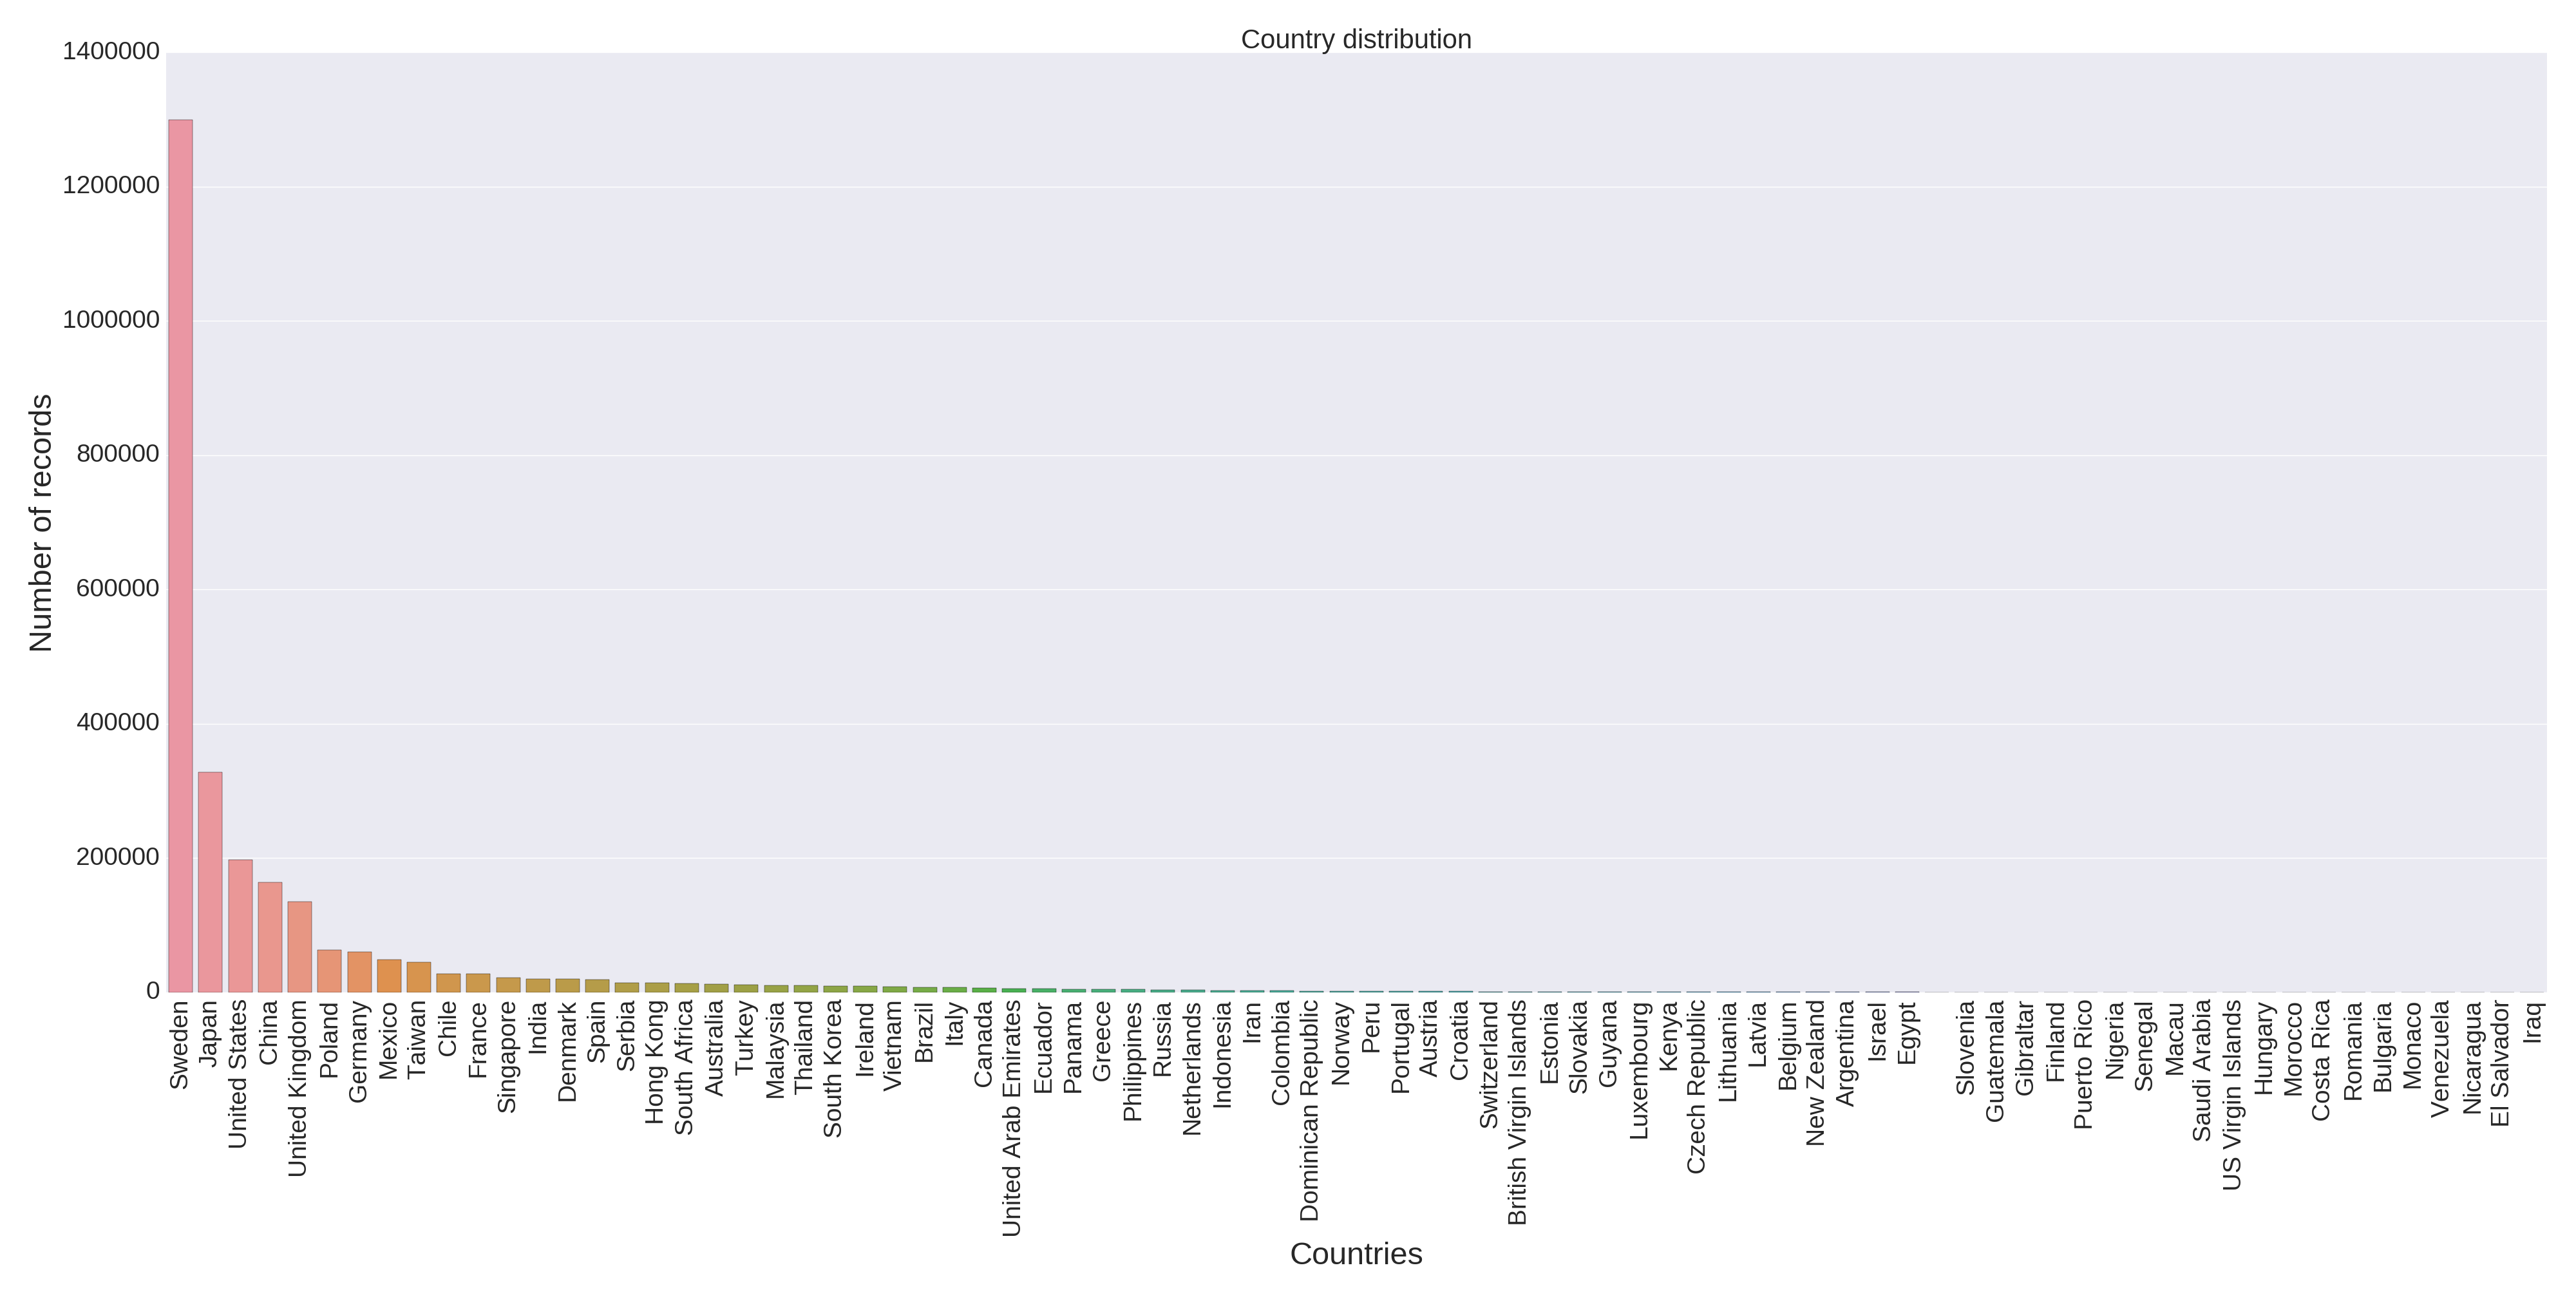
\includegraphics[scale=0.14]{country_distribution}
    \caption{Distribution for number of location updates between the five countries with most updates}
    \label{fig:country_dist}
\end{figure}


That Sweden and Japan are the top of the list is not strange as Sony is a Japanese company which took over Sony-Ericsson where Ericsson is a Swedish company. Sony-Ericsson was at that time the mobile brand of Sony, so a large part of Sony's mobile development is still placed in Sweden. This may explain why Sweden has three times as many updates as Japan.  

On the basis of figure \ref{fig:country_dist}, we will look at the data of Sweden and Japan going forward. Now the data for the two countries will be compared. 
In Japan there are \numberUsersJapan{} unique users while in Sweden there are \numberUsersSweden{}. The two countries may have common users as users may travel between several countries and thereby have location updates in several countries.  
In the total number of location updates Japan has \locUpdatesJapan{} updates, whereas Sweden has \locUpdatesSweden{} updates for all three months. 

Figure \ref{fig:mean_loc_updates_sep-nov} compares the mean value of location updates in Japan and Sweden. 

\begin{figure}[H]
    \hspace*{-2.2cm}
    \centering
    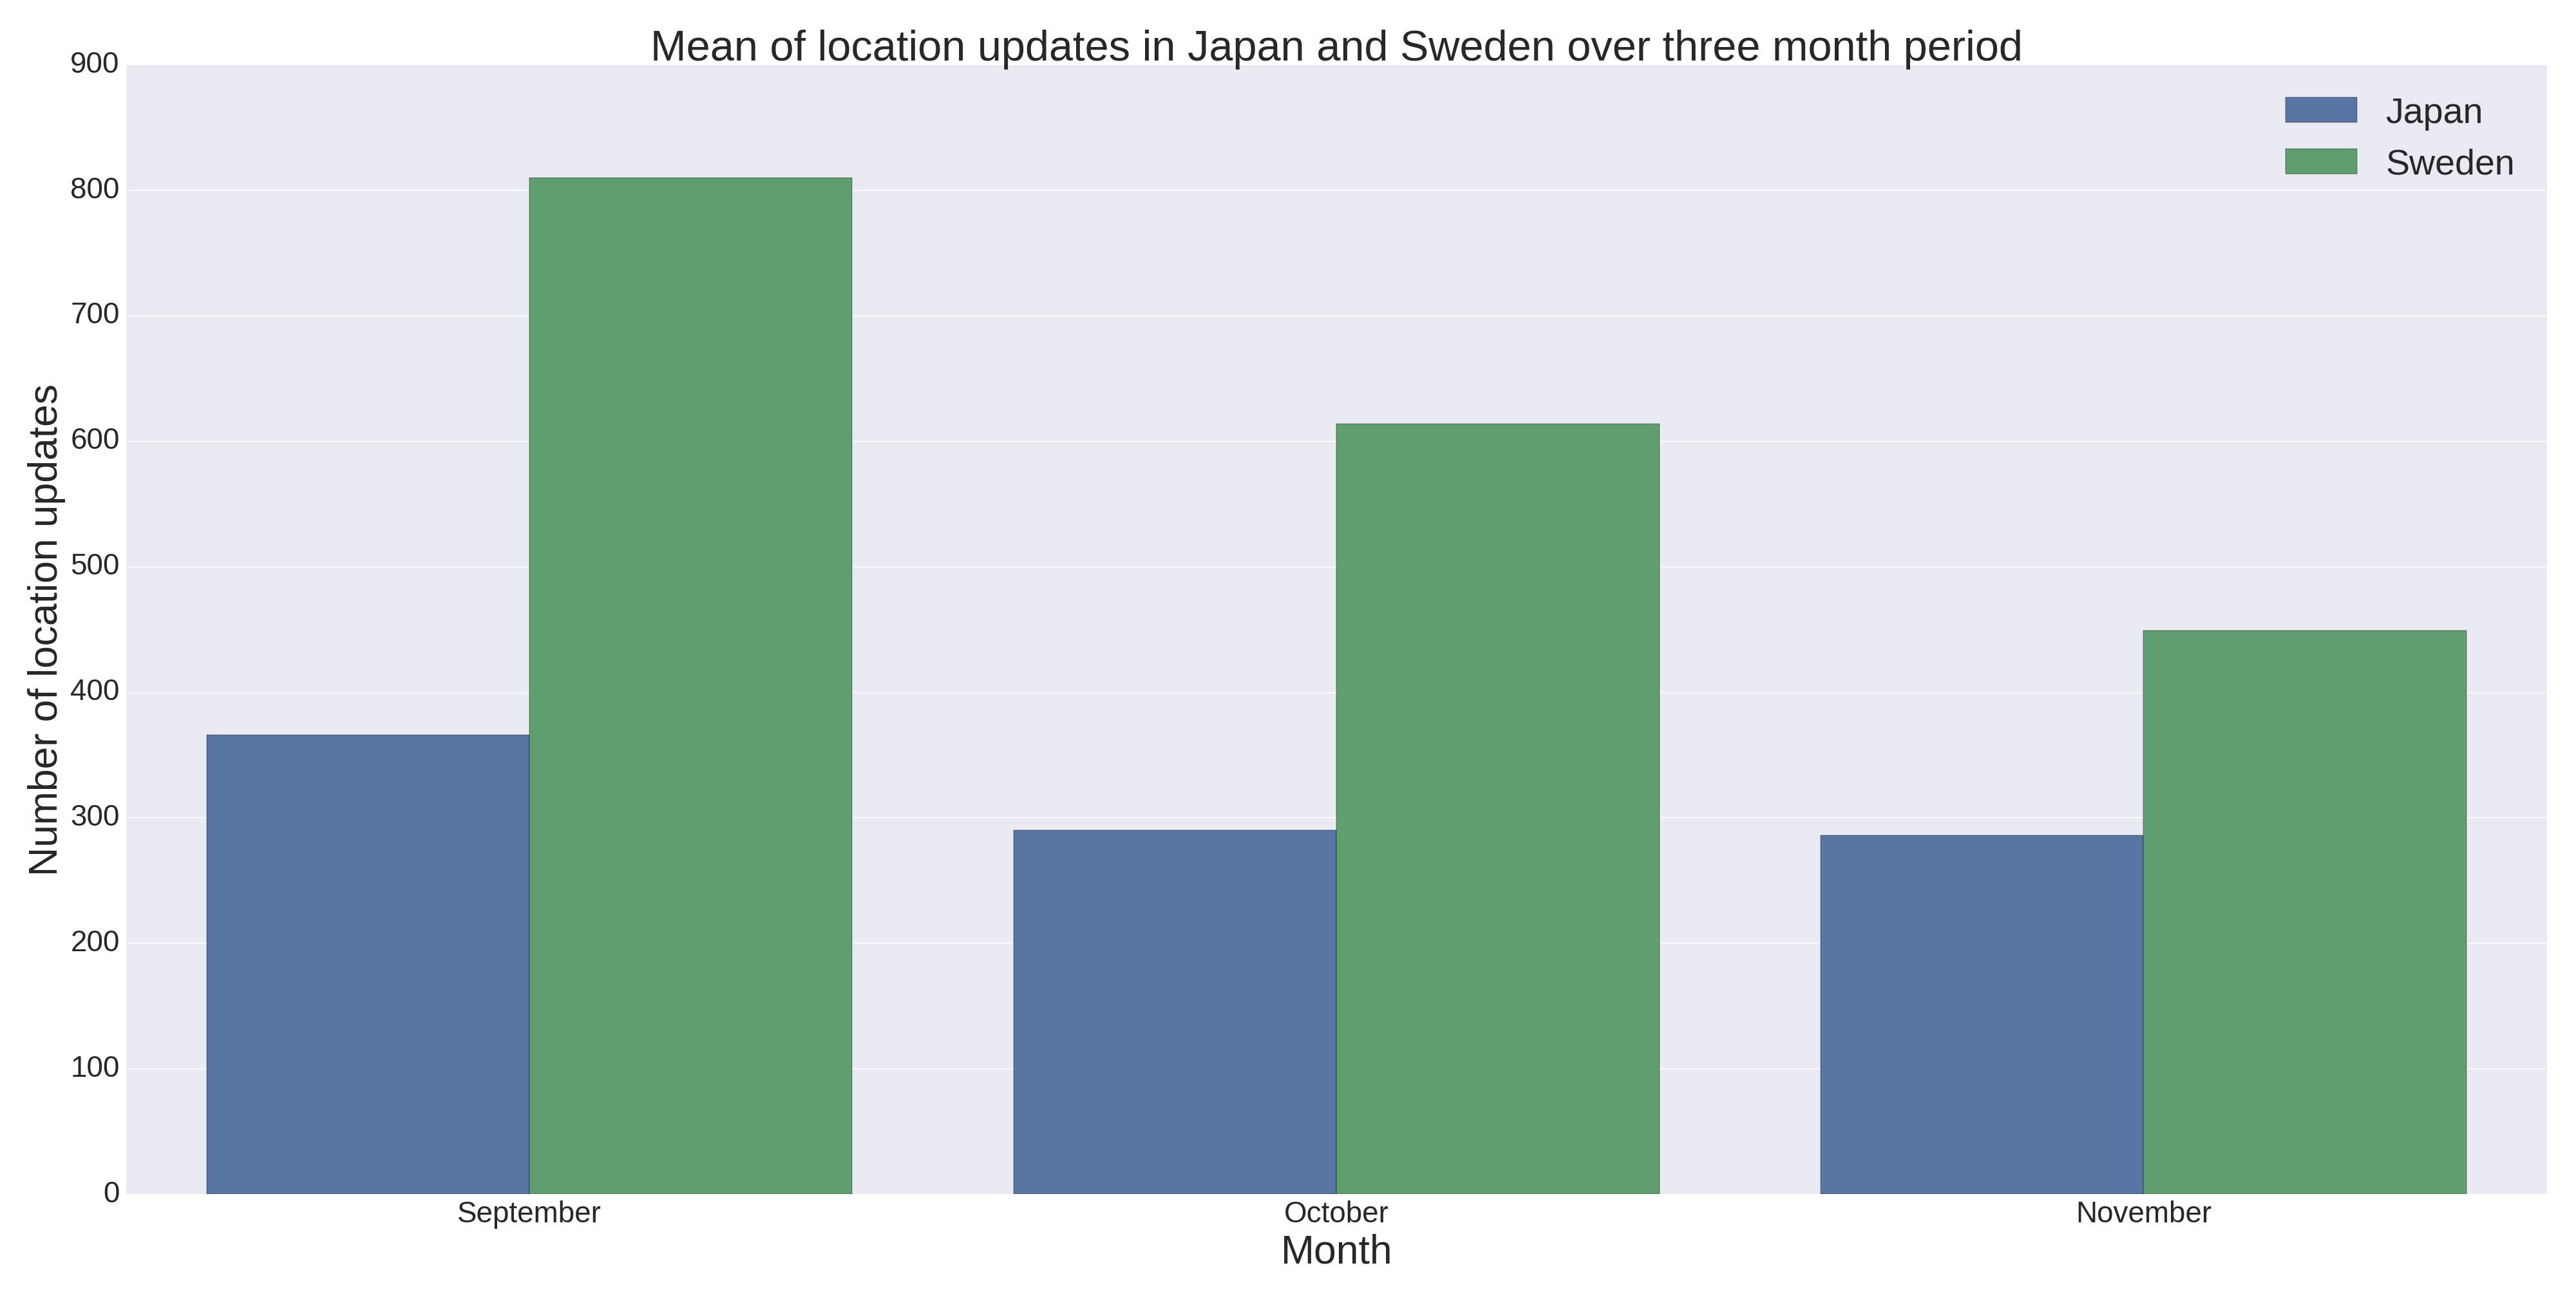
\includegraphics[scale=0.16]{mean_loc_updates_sep-nov}
    \caption{Distribution for mean of location updates for Japan and Sweden}
    \label{fig:mean_loc_updates_sep-nov}
\end{figure}


We can see that Sweden has significantly more updates than Japan during all three months and in the two months September and October even twice as much. We can also see a decreasing tendency in both countries. September has the highest number of updates and thereafter the number decreases, where November in Sweden has more that 300 updates less than in September. Even as the tendency is more prominent for Sweden it is also visible for Japan.  \\
This will be investigated more closely later.  


As mentioned earlier there are some natural gathering places in Sweden and Japan, as the data are for Sony employees. These places are of course work-related, such as Sony's offices in the two countries. Three places in Sweden and one in Japan has been identified. The reason for the importance of this is that peoples co-occurrences are work related, which not necessarily mean that they are friends with a person with whom he has a co-occurrence. 

It is therefore interesting to see how many updates for each country are made inside these gathering places and how many are outside.  

\begin{figure}[H]
    \hspace*{-2.2cm}
    \centering
    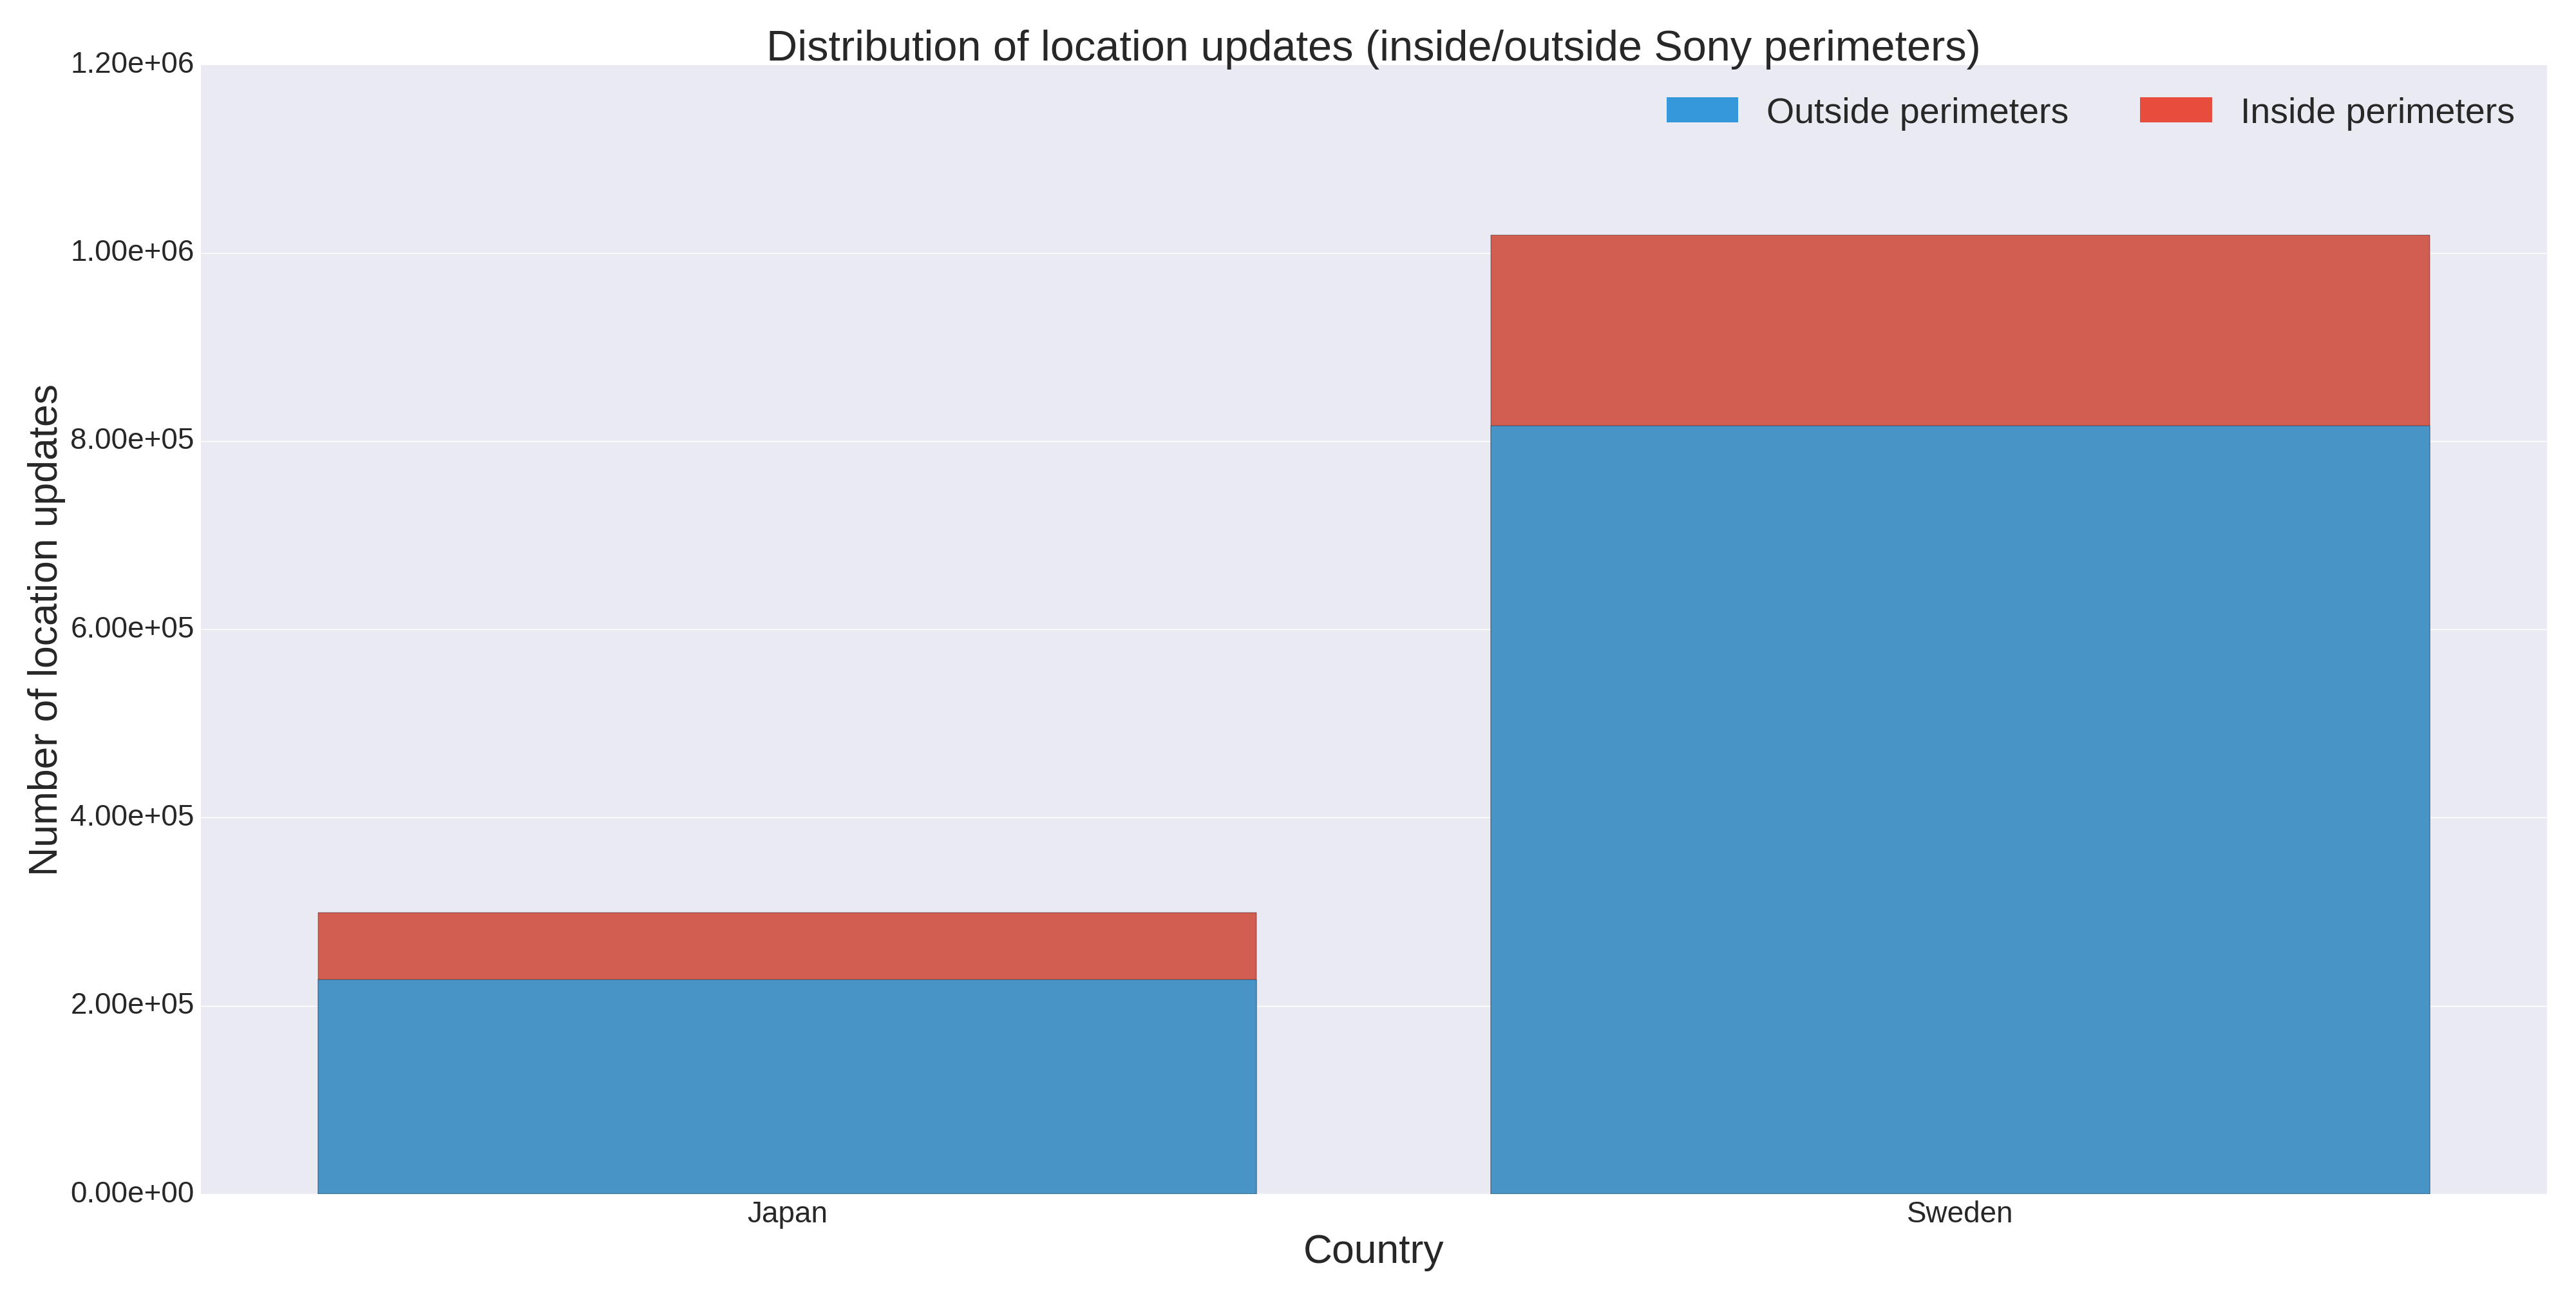
\includegraphics[scale=0.16]{stack_bar_loc_updates}
    \caption{Shows how many of the updates that is outside/inside Sony perimeters}
    \label{fig:hq_stack_bar}
\end{figure}

Figure \ref{fig:hq_stack_bar} show how updates are distributed with respect to whether they are made on a gathering place or not. It can be seen for both countries that there is a reasonably small proportion of updates inside gathering places. For Japan and Sweden this value is 23.89\% and 19.86\% respectively. 
It looks good for the thesis that such a large amount of updates are outside the gathering places. 

For each of the two countries the distribution of the updates between the users is of interest. For this purpose the quantiles for each country are available in Table \ref{tab:stat_loc_updates}. 


\begin{table}[htbp]
        \centering
        \small
        \setlength\tabcolsep{2pt}
        \begin{tabular}{|c|c|c|c|c|c|c|c|c|c|c|}
            \hline
                         & Japan      &   Sweden      \\[-1pt]
            \hline
                 Min     &    1       &   1           \\
            \hline
                 Q1      &  26        &   68      \\
            \hline
                 Median  & 233     &   840      \\
            \hline
                 Mean    &  851.49   &  1,735.38     \\
            \hline
                 Q3      & 994.5    &   2,642     \\
            \hline
                 Max     &  9,320 &  14,759     \\
            \hline
                 IQR     &  968.5   &   2,574     \\
            \hline
            
        \end{tabular}
        \caption{Quantiles and mean over location updates for Japan and Sweden} %add this between 'caption' and '{...' for new text in listing of tables: [New caption text only for listing of tables]
        \label{tab:stat_loc_updates}
\end{table}


When we look upon the quartile of the countries, we can see that the 25\% quantile (Q1) is very low in both countries. Q1 shows in other words that 25\% of the users in Japan and Sweden respectively has less than 26 and 68 updates during these three months. It is not a good condition that so many users have so few updates. The 75\% quantile (Q3) is a good deal higher in Sweden than in Japan, which shows that there are 75\% of the users who has a maximum of 994.5 and 2,642 location updates in Japan and Sweden respectively. Again the data seems better in Sweden where the users have more updates than in Japan. \\ 


Both countries has a small percentage of users having extraordinary many updates. In Sweden there are 25\% users who have between 2,642 and 14,759 updates and in Japan they have between 994.5 and 9,320 updates. As with Q1 this is a bad sign. 
Median and mean are very much larger in Sweden than in Japan. This indicates that there are more users with many updates in Sweden than in Japan.  \\

The tendency described above can be shown more clearly by plotting the Cumulative Distribution Function (CDF) for the two countries.  
 
\begin{figure}[H]
    \hspace*{-1.0cm}
    \centering
    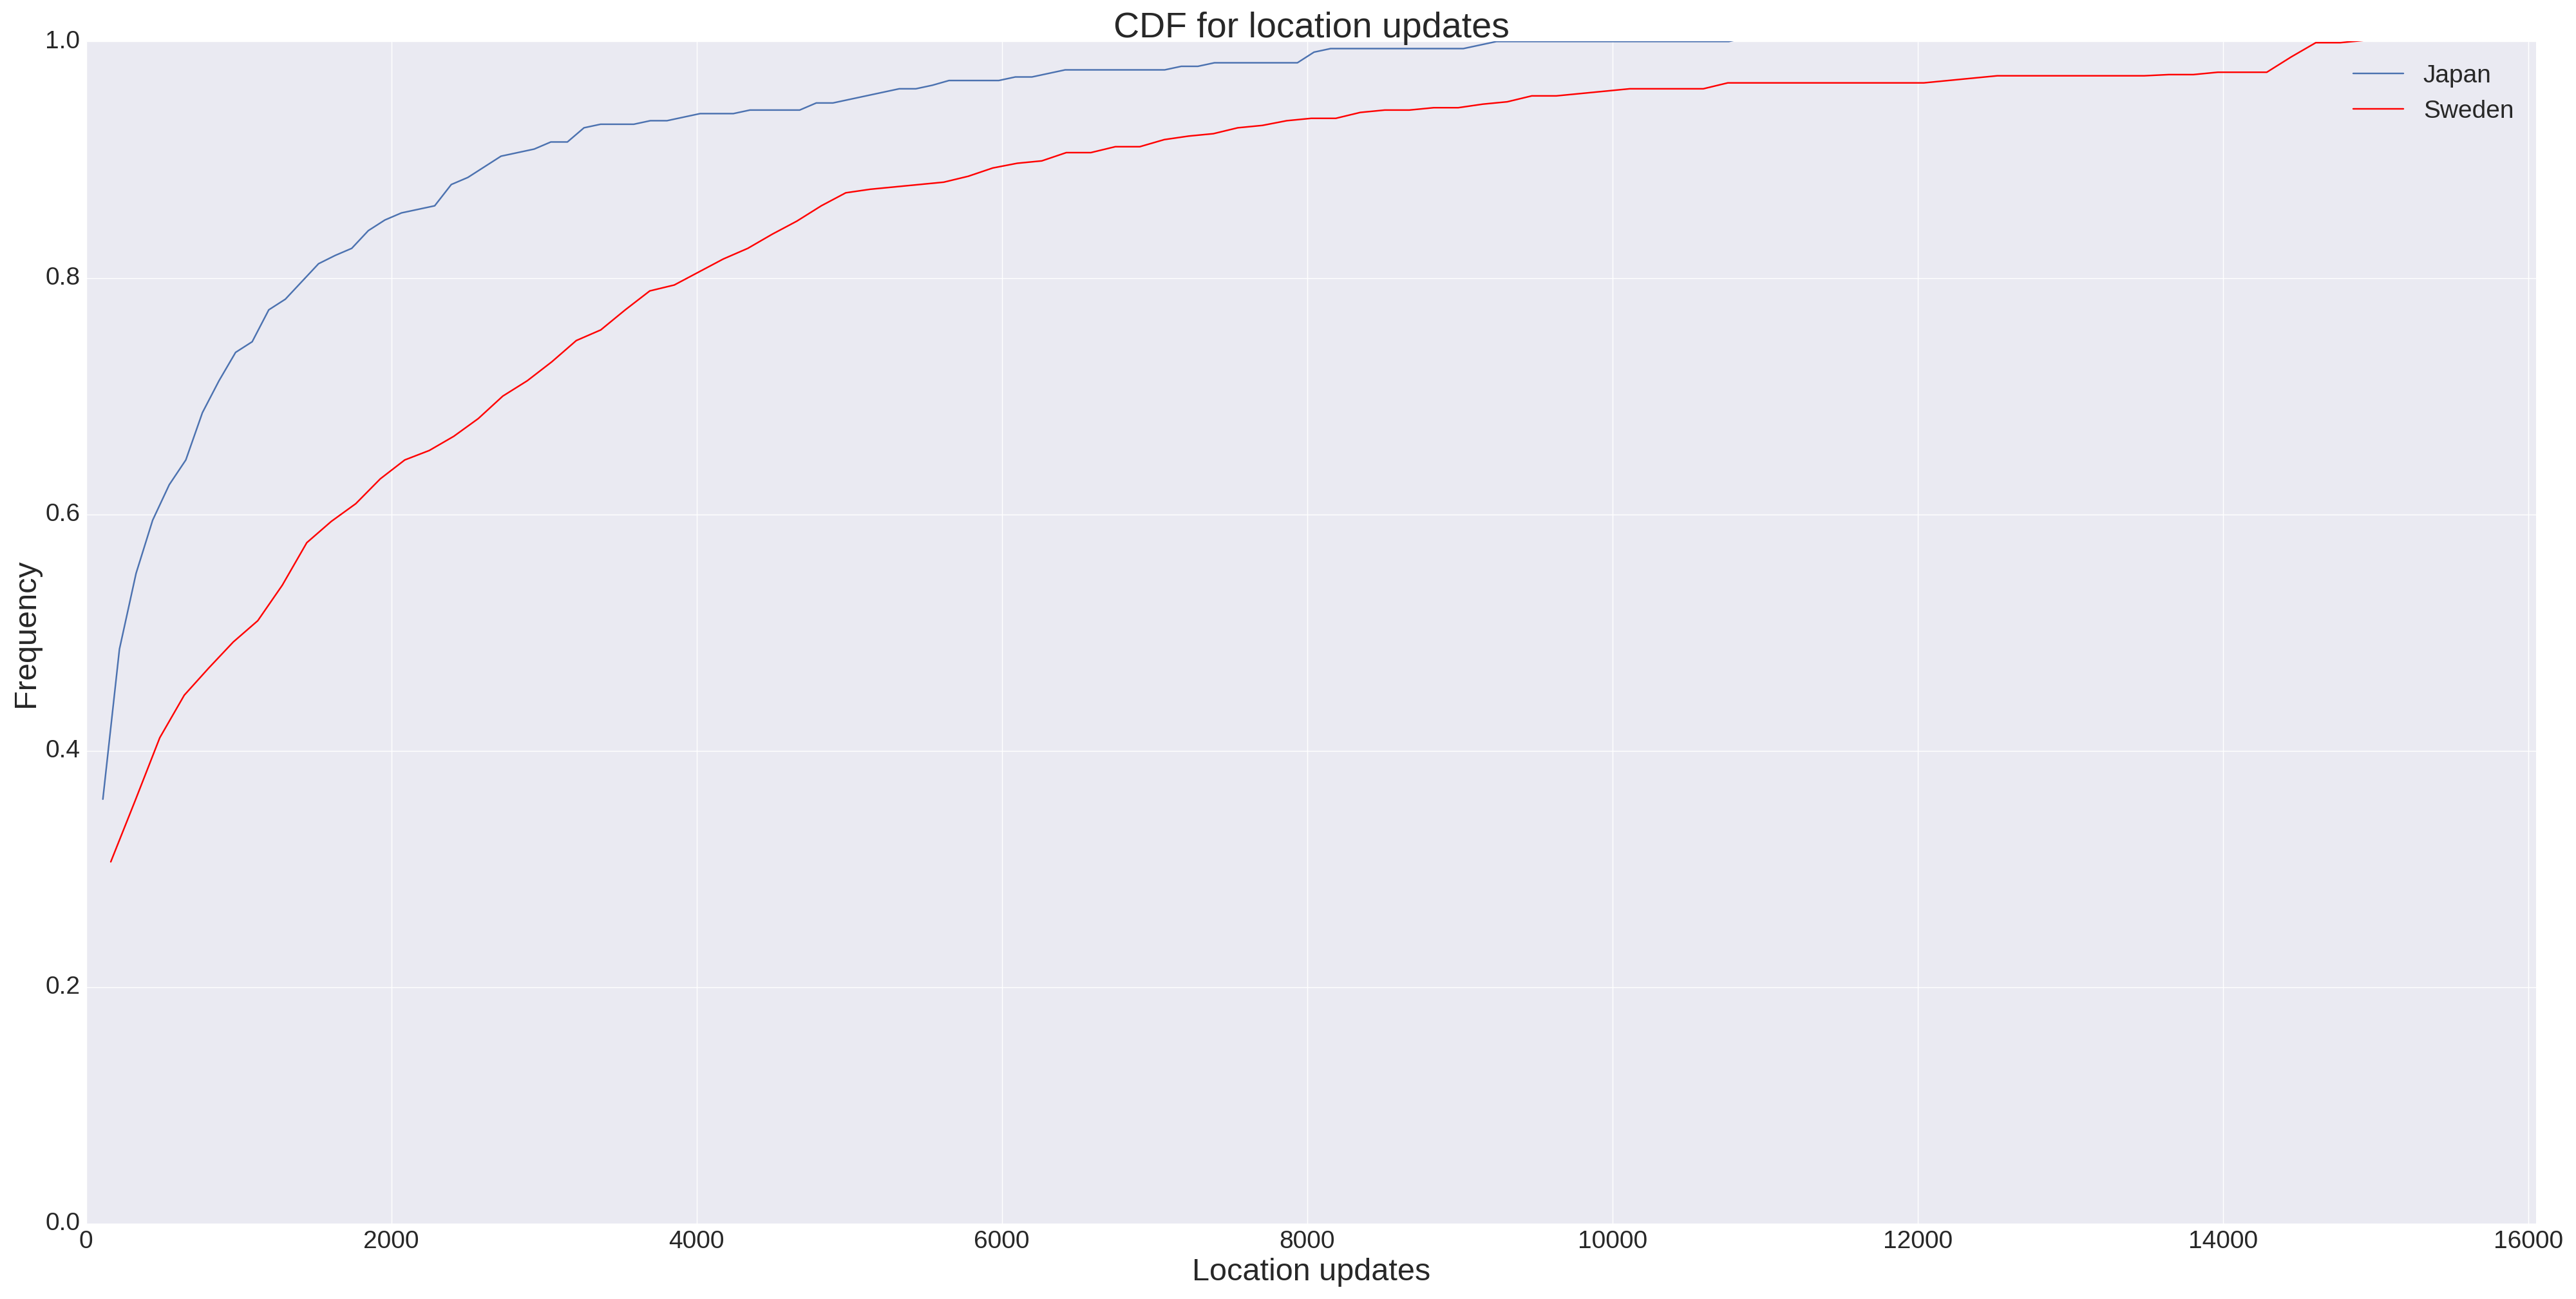
\includegraphics[scale=0.14]{cdf_location_updates_swe_jap}
    \caption{Cumulative Distribution Function (CDF) over location updates for Japan and Sweden over the three months of the period}
    \label{fig:country_cdf}
\end{figure}

The plot shows that in both Japan and Sweden there are a large part of the users with very few location updates during the whole period. It can be seen that in Japan the number of users with few updates increases faster than in Sweden.  
As the updates are generated each time the user changes his location, it must indicate that many of the users are very stationary or they have turned off their mobile phones. It must be stated that stationary also encompasses the situation where the user has forgotten his phone at home. In the data we can see the difference between whether the phone has been switched off or is stationary, but not whether the phone is stationary or just forgotten. We can differentiate between the situation with a phone turned off and a stationary phone by noting that in the first case data are missing for a while whereas with a forgotten phone there is a long time between \texttt{start\_time} and \texttt{end\_time}.  

It is important to see if there is a pattern in the time-stamp of the updates, as it may be possible on this background to identify better or worse sub-periods, which may be taken into account. 
We have plotted heat maps for how the updates are distributed over 24 hours. These are produced by aggregating data from a time slot in a 24 hour period. The aggregated data are based on whether the user has had at least one update in the time slot of the day (represented by 0 or 1), regardless of which day it is. 

\begin{figure}[H]
    \hspace*{-0.8cm}
    \centering
    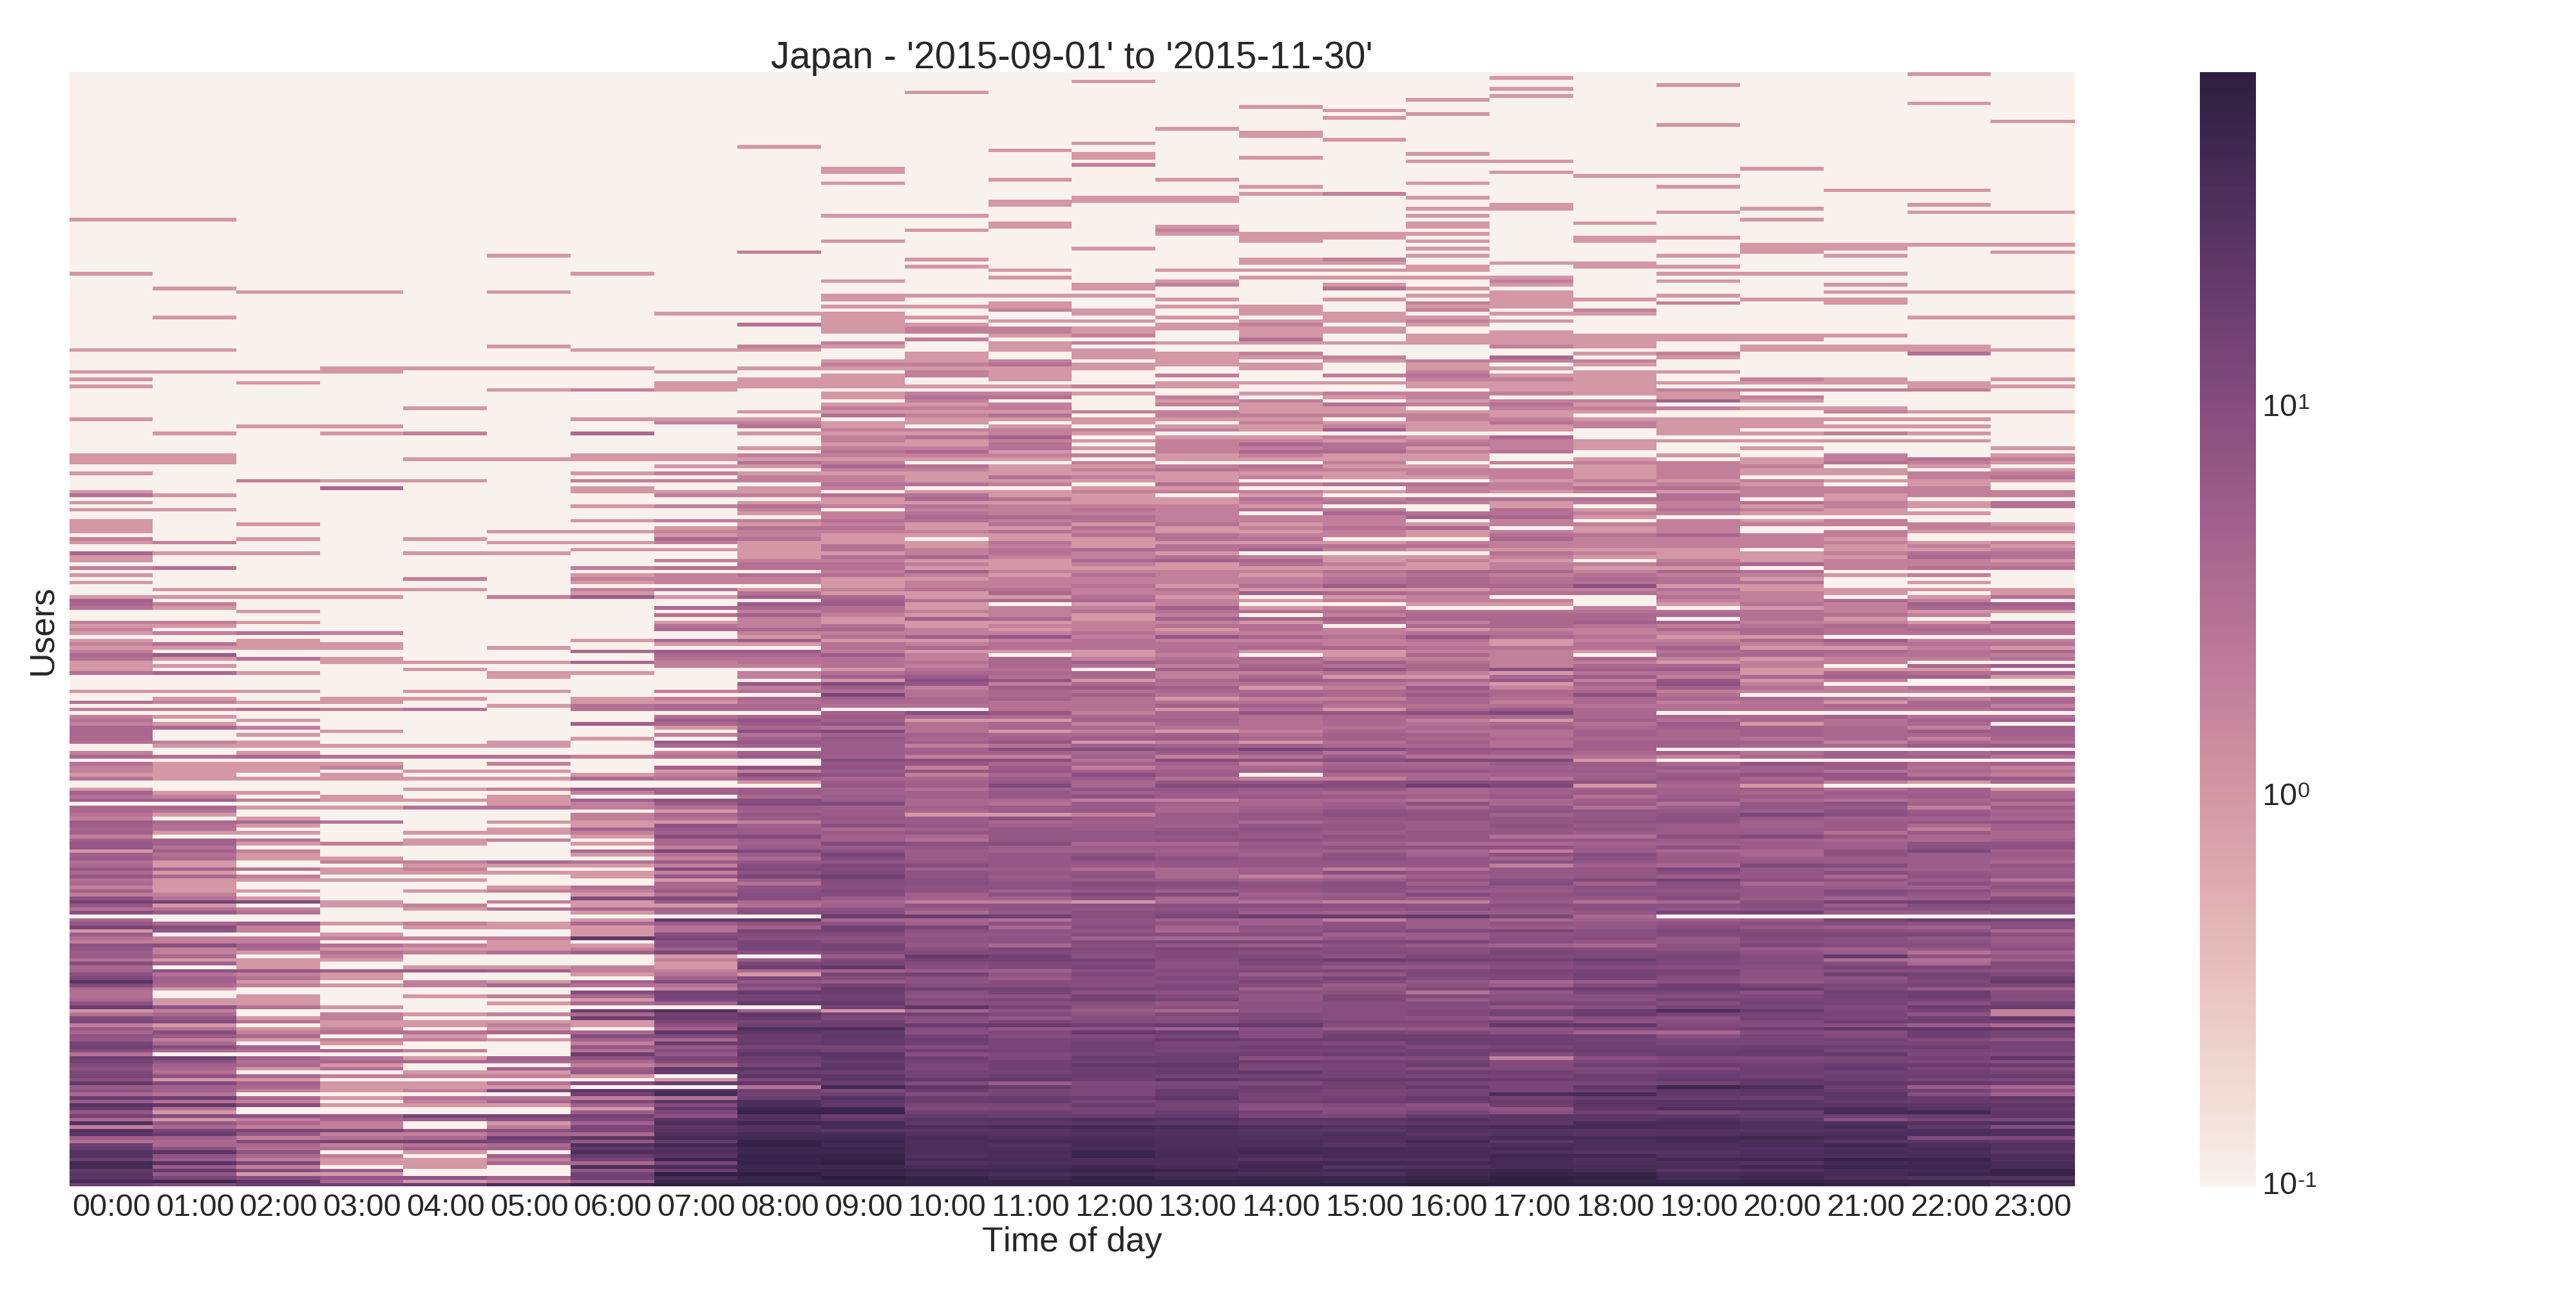
\includegraphics[scale=0.15]{aggregated_updates_over_time_japan}
    \caption{Heat map for location updates over the 3 month period in Japan, aggregated over a day with 60 minutes of bin size. Users are sorted by total values. Largest is at the bottom. The scale is logarithmic}
    \label{fig:agg_heatmap_jap}
\end{figure}
Figure \ref{fig:agg_heatmap_jap} shows how updates for each user (y-axis), are distributed over the time of day, measured over all 3 months. The users are sorted according to their total aggregated values, with the largest at the lowest part of the Y-axis.  

We see clearly that there is a period between 02:00 AM and 06:00 AM where most users do not have any updates, which might indicate that they either turn the mobile off or otherwise shuts down the communication with the external world in the mentioned period. From this time 06:00 AM until 12:00 PM there are regular updates after which time the number of updates decreases until 02:00 AM. If we compare this with Figure \ref{fig:cumu_loc_time_jap_swe} we can see a reasonable good correlation. Figure \ref{fig:cumu_loc_time_jap_swe} shows the  aggregated location updates over 24 hours in both Japan and Sweden. In this we see the same development in Japan as the heat map indicates, as described above. 

The above mentioned is also valid for Sweden (Figure \ref{fig:agg_heatmap_swe}), which show the same as for Japan. Also here almost all users turn their mobiles off between 02:00 AM and 06:00 AM. 
No other time slots have a significant deviation neither in Japan nor in Sweden.  

As the users have been sorted, we can easily see that a part of the users do not have any or very few updates during all three months. These users are discarded in the test data as they do not contribute with a significant amount of data.  

When we initially plotted Figure \ref{fig:agg_heatmap_swe}, we discovered 16 users with an identical number of location updates in every hour period, upon further investigation we discovered the users all had duplicate location updates. We removed the users from the dataset as they were likely test-users from Sweden.

\begin{figure}[H]
    \hspace*{-0.8cm}
    \centering
    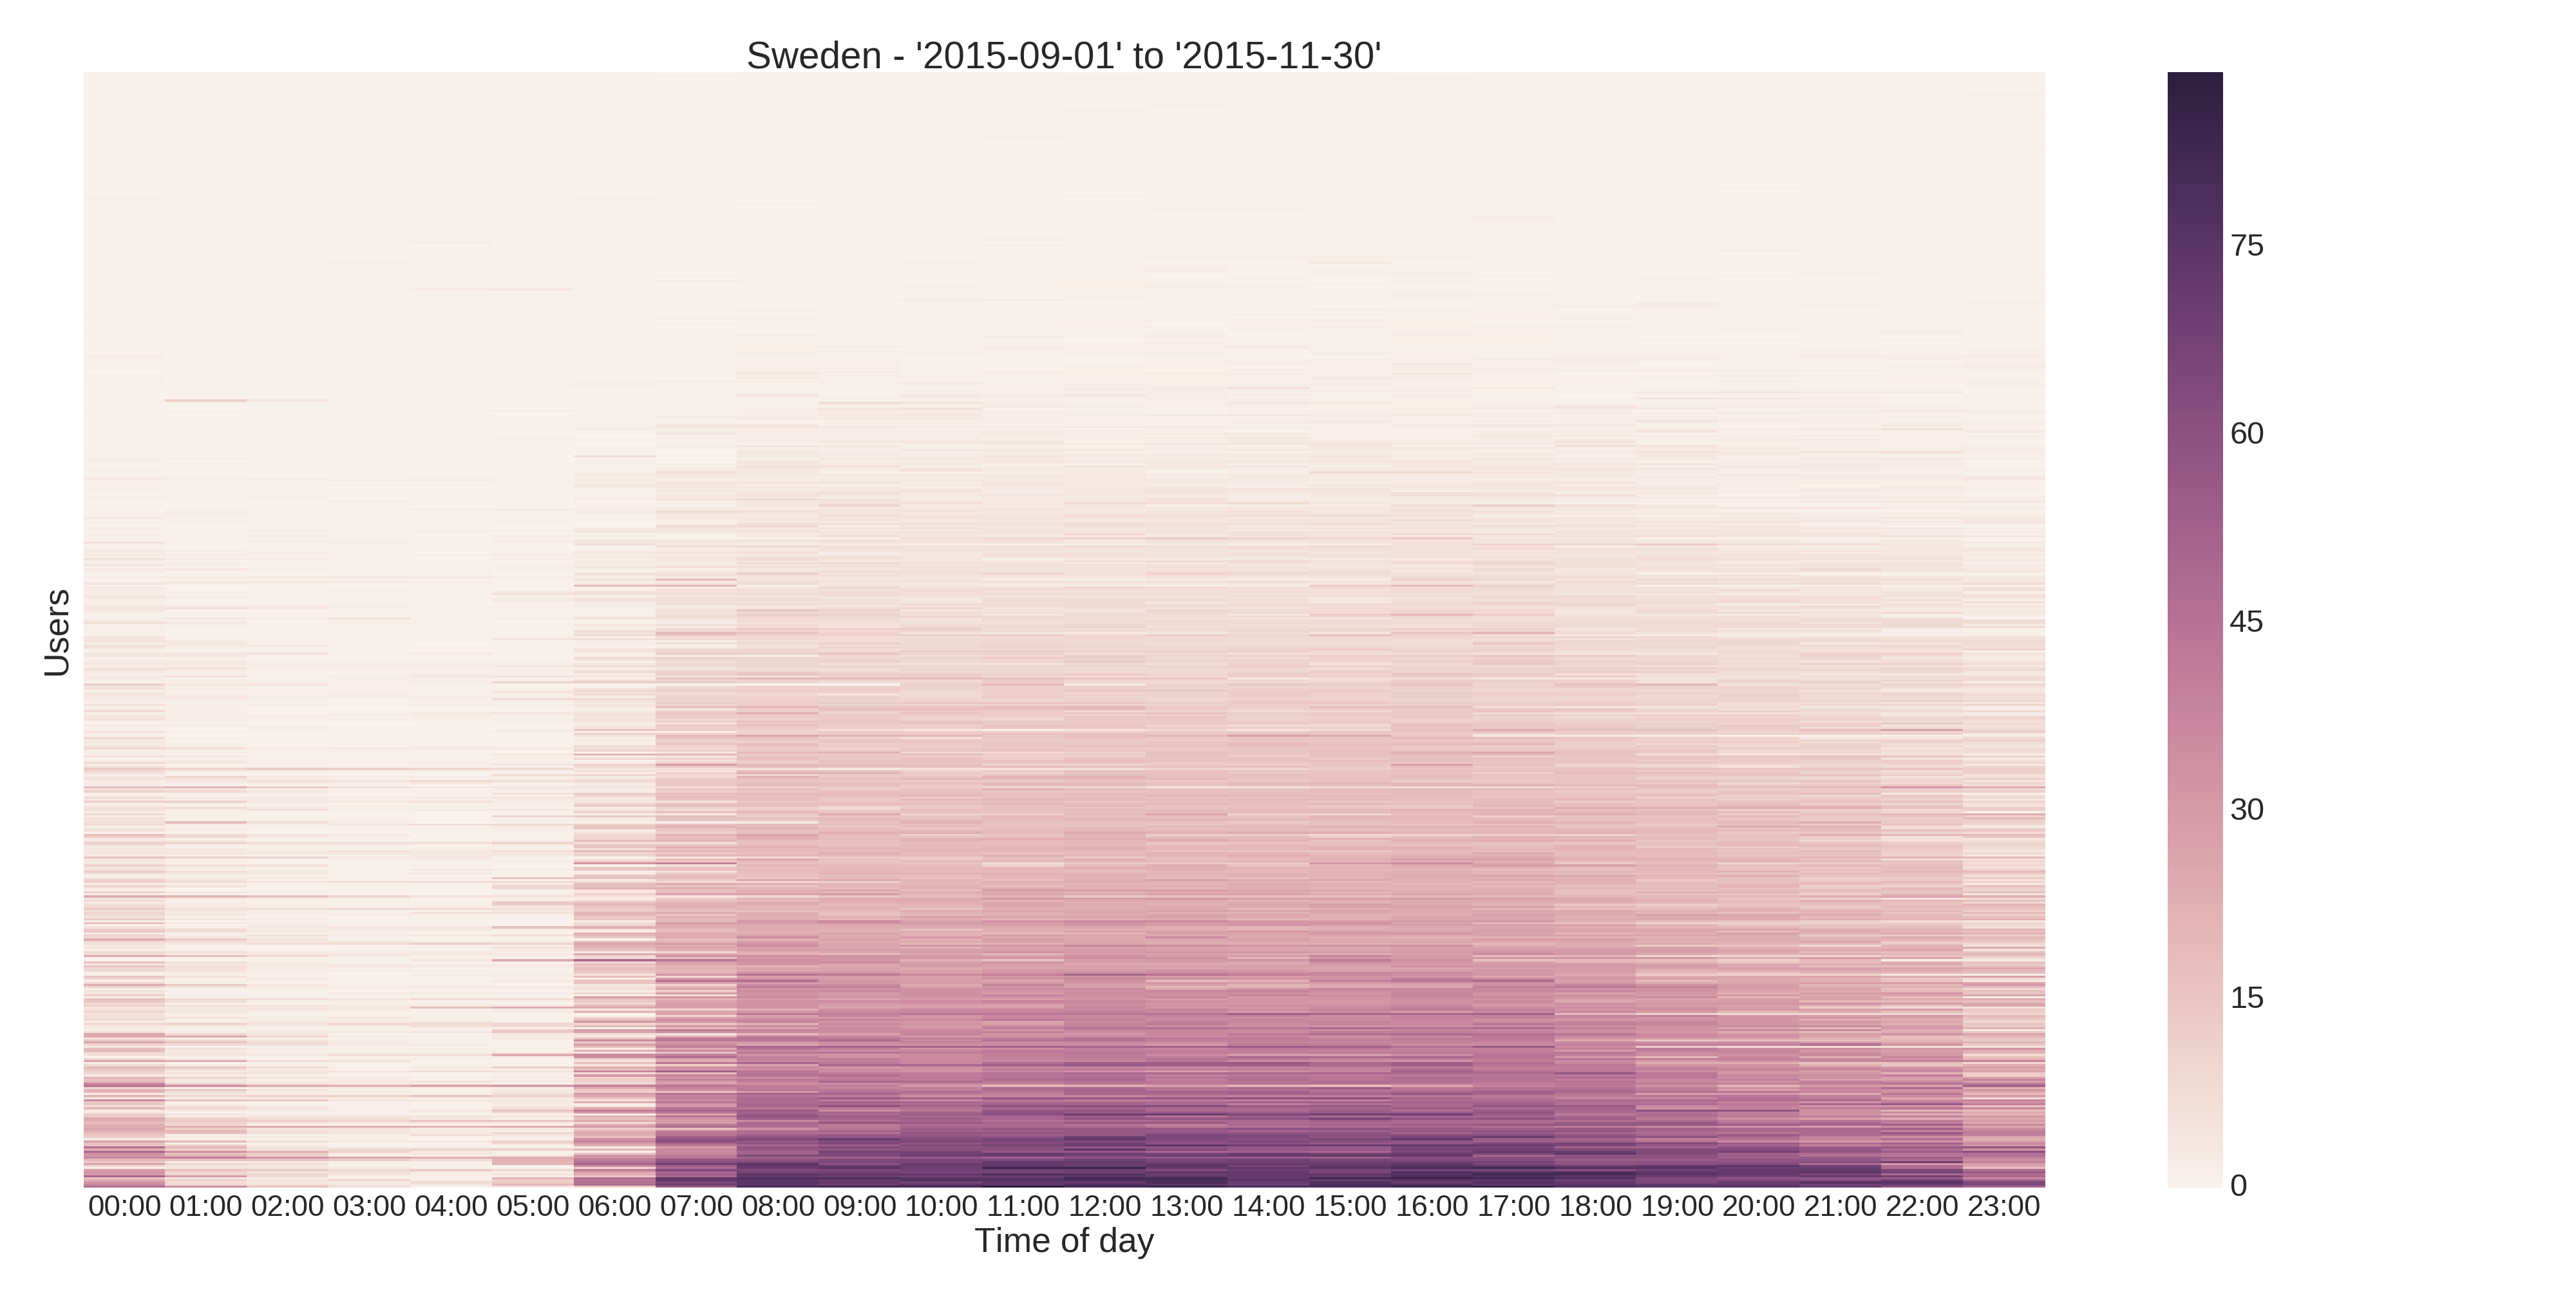
\includegraphics[scale=0.15]{aggregated_updates_over_time_sweden}
    \caption{Heat map for location updates over the 3 month period in Sweden, aggregated over a day with 60 minutes of bin size. Users are sorted by total number of location. Largest is at the bottom}
    \label{fig:agg_heatmap_swe}
\end{figure}

\begin{figure}[H]
    \hspace*{-1.8cm}
    \centering
    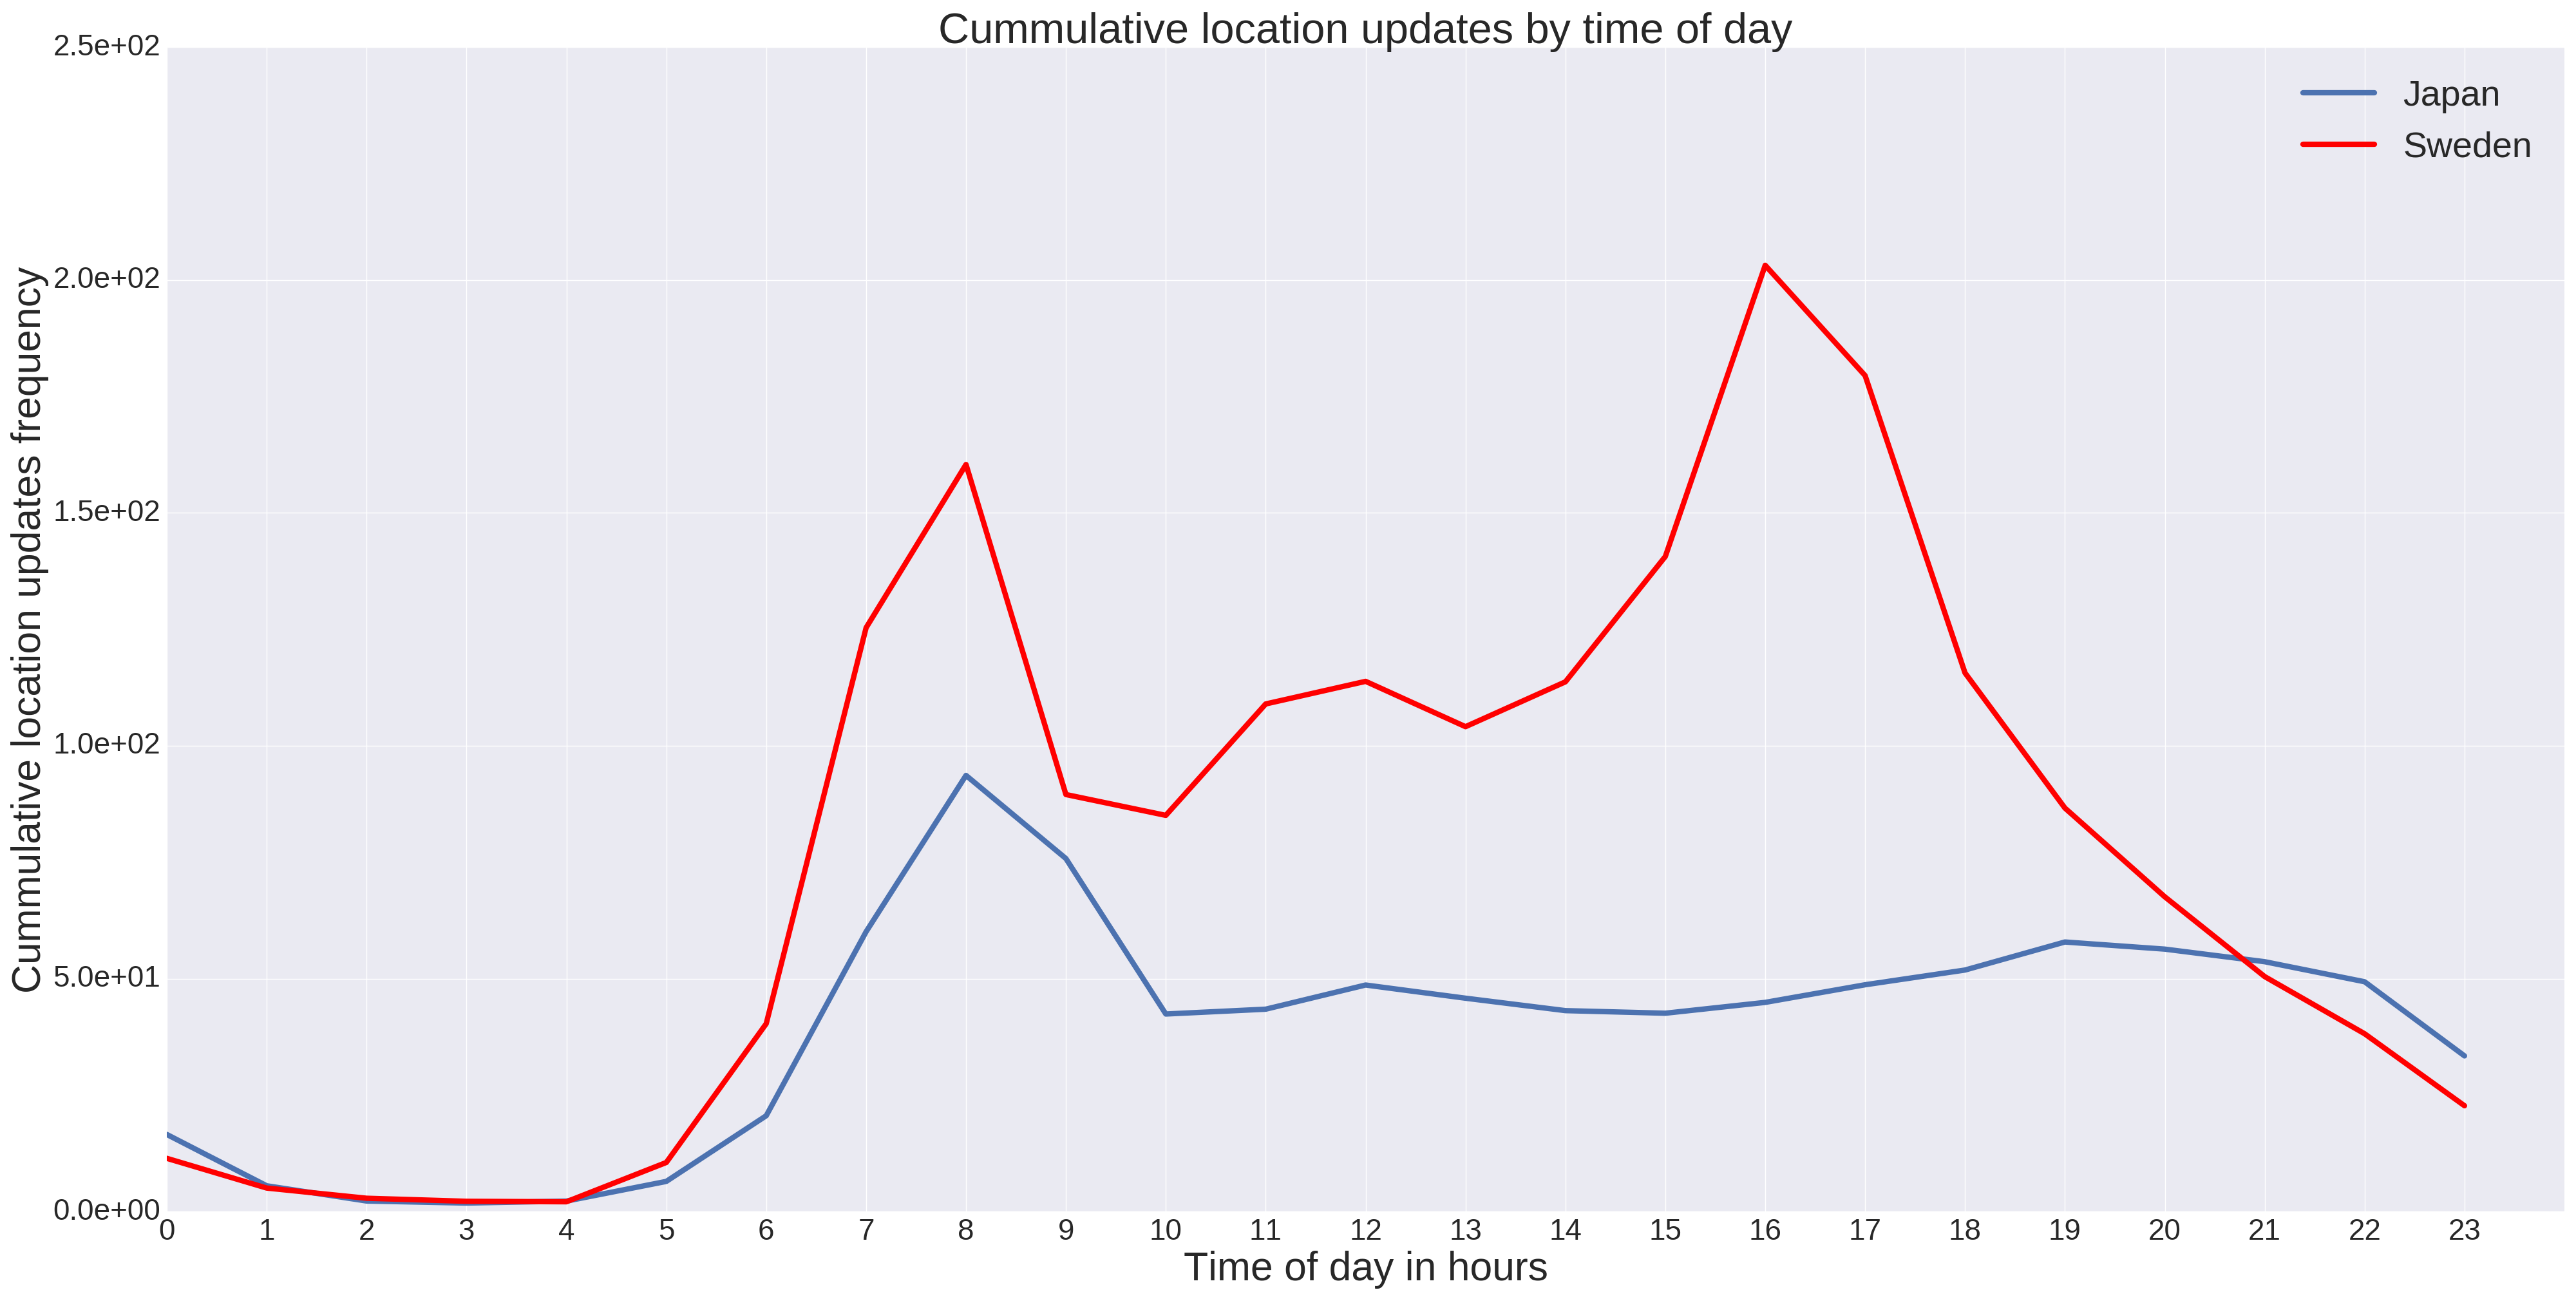
\includegraphics[scale=0.15]{cumulative_updates_overTime_swe_jap}
    \caption{Shows when the cumulative location updates occurring over a day. The value of the updates are normalized}
    \label{fig:cumu_loc_time_jap_swe}
\end{figure}

If we only look at Figure \ref{fig:cumu_loc_time_jap_swe}, we can see that in both countries the number of updates have a peak at about 08:00 AM. In Sweden there is a further peak at 04:00 PM whereas in Japan there is no similar peak. \\
The peak at 08:00 AM may be caused by users moving from home to work and in this process generates a lot of updates. Similarly the second peak (in Sweden) may be caused by users returning to their home again generating a certain number of updates. It can be remarked that Japan does not have a similar increase in location updates in the afternoon, but a slight increase at 7:00 PM and higher values than Sweden from 21:00 PM until 01:00 AM. \\

Figures \ref{fig:agg_heatmap_jap}, \ref{fig:agg_heatmap_swe} and \ref{fig:cumu_loc_time_jap_swe} tell which times of the day may be more usable than others. For instance that it is important to be aware of the time between 01:00 AM and 06:00 AM, as many users have very few updates in this period. It will probably mean that this period should be avoided. 
What the figures do not tell, is whether there are days in the three months which are better than others. This issue is interesting to investigate to see whether there are some days which might be used with advantage instead of using all days. Furthermore it might be possible to see a pattern for the days. We can imagine that on Fridays and/or Saturdays there are more updates than on other days because people get together in town and because of this are active.  


\begin{figure}[H]
    \hspace*{-1.5cm}
    \centering
    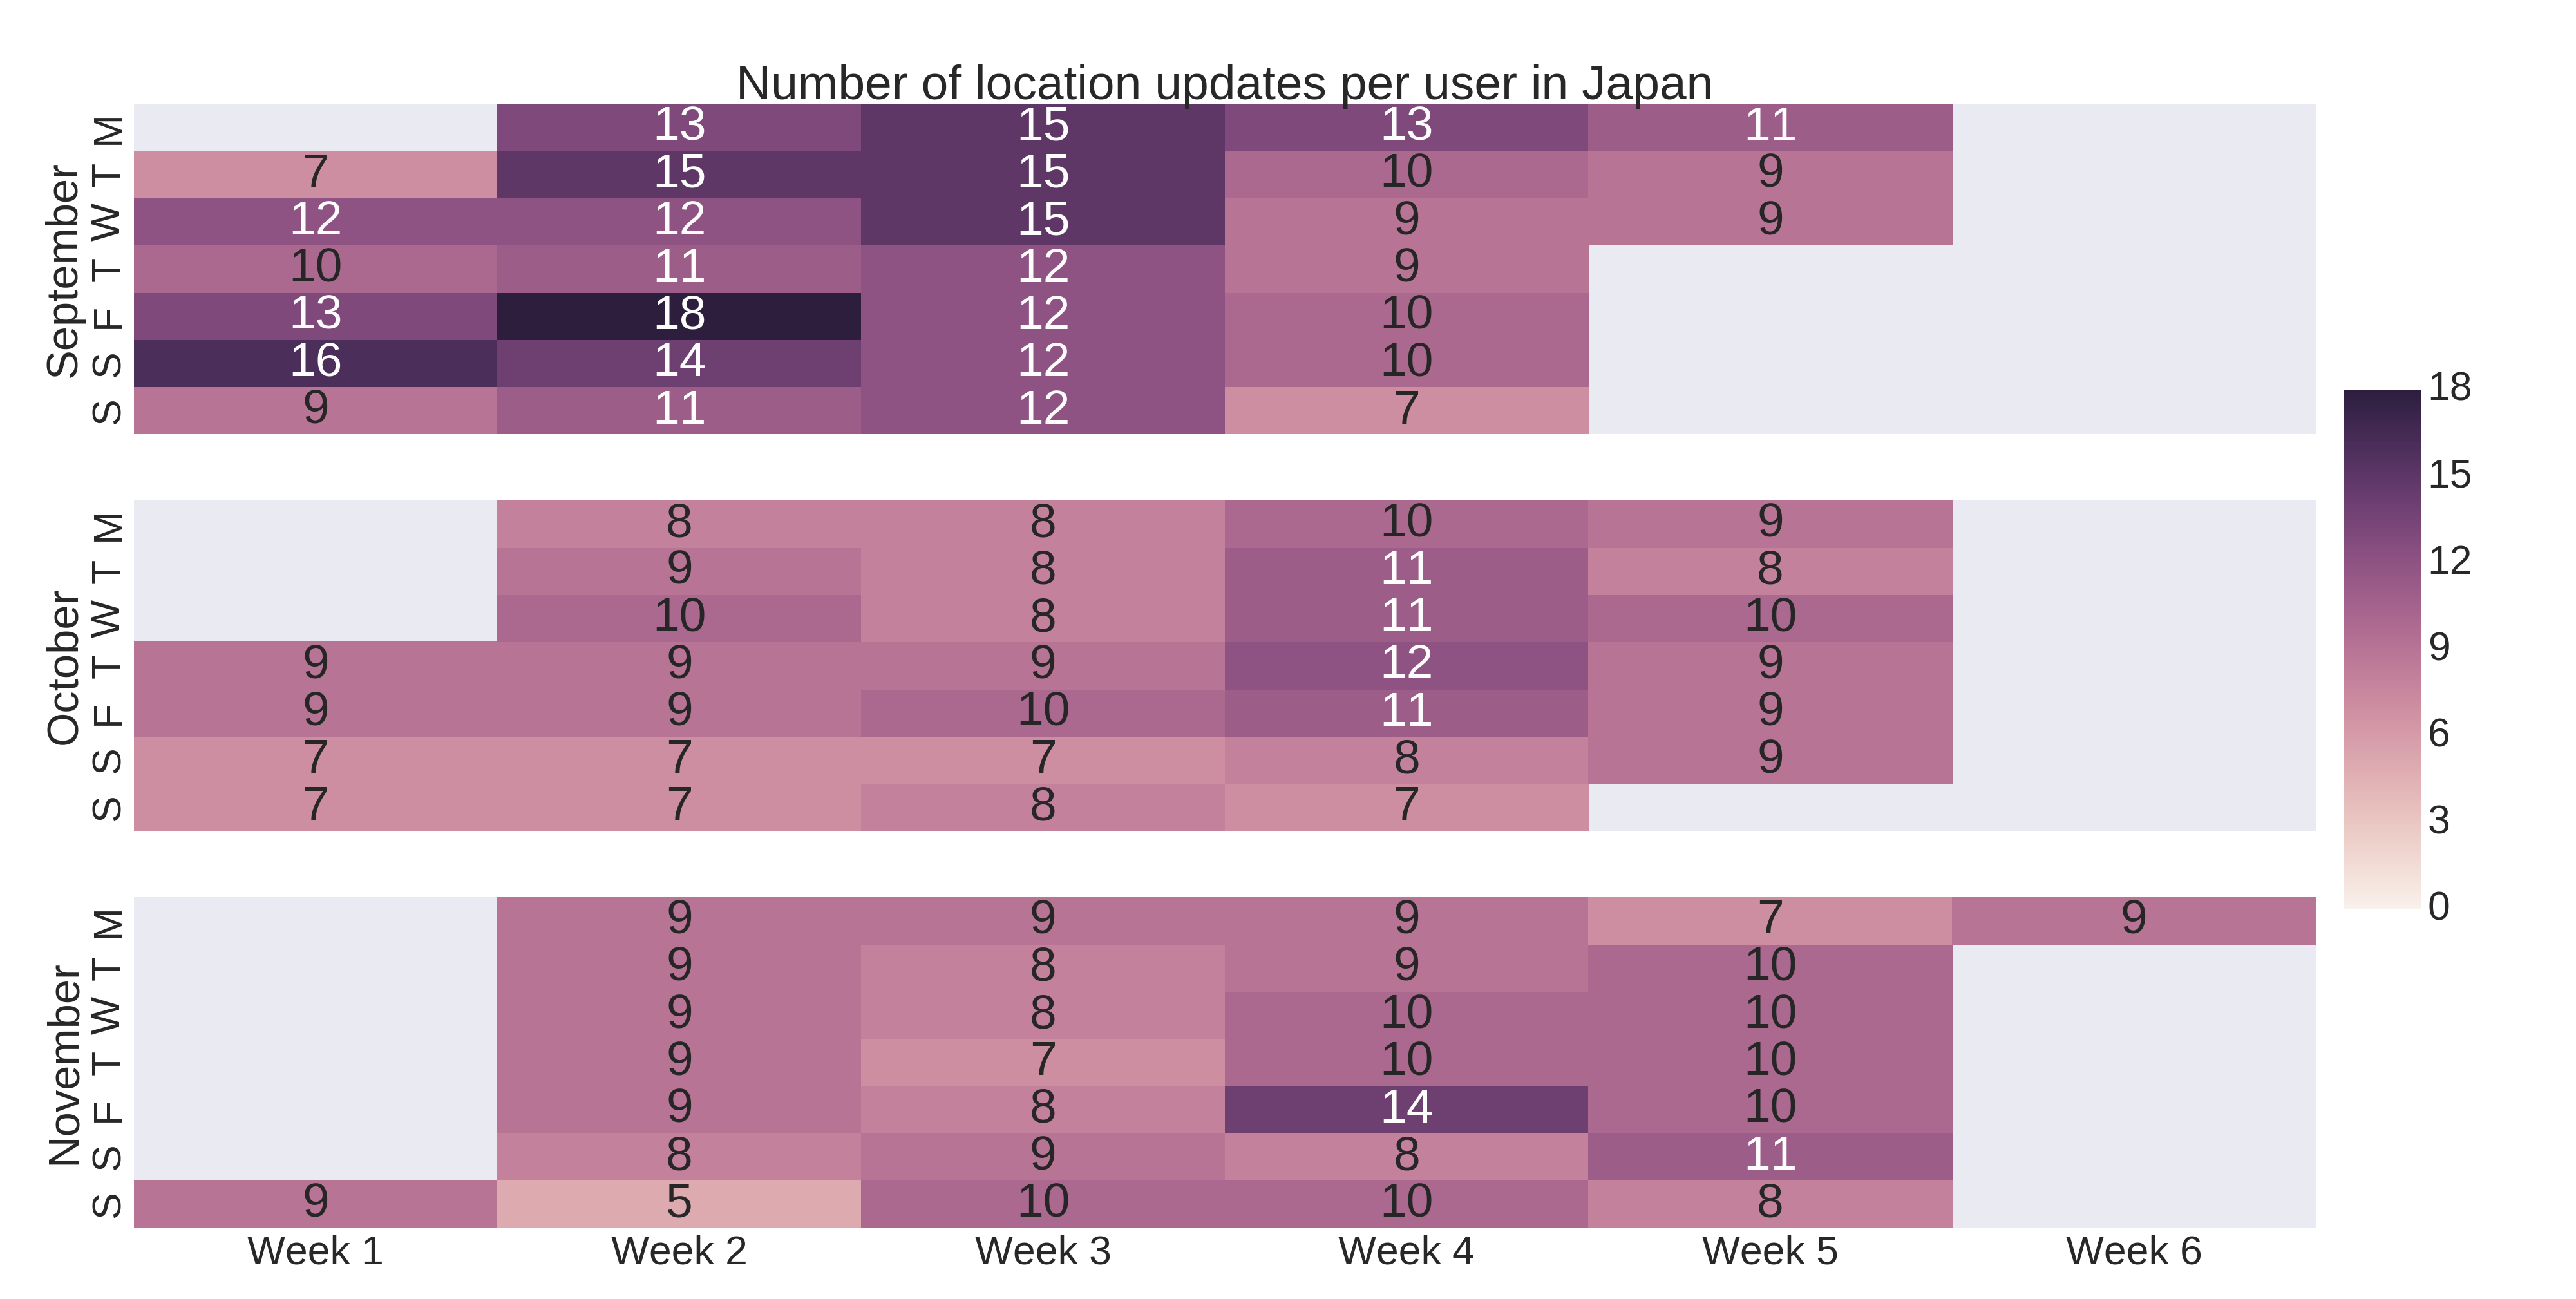
\includegraphics[scale=0.15]{heatmap_location_updates_japan}
    \caption{Heat map for mean location updates over the 3 month period in Japan}
    \label{fig:heatmap_jap}
\end{figure}

Figure \ref{fig:heatmap_jap} shows how location updates per user in Japan (rounded to nearest integer) is distributed for each day in each of the three months. We can for example see that in Japan we have as a mean 16 updates per user on Friday in week 2 of September.  

Again we see that generally there are more updates in September than in the other two months. October and November are similar apart from some days where November has some higher values than some other days in October. 

In many cases we can see that Fridays and/or Saturdays have higher values than other days in the same month. 

\begin{figure}[H]
    \hspace*{-1.5cm}
    \centering
    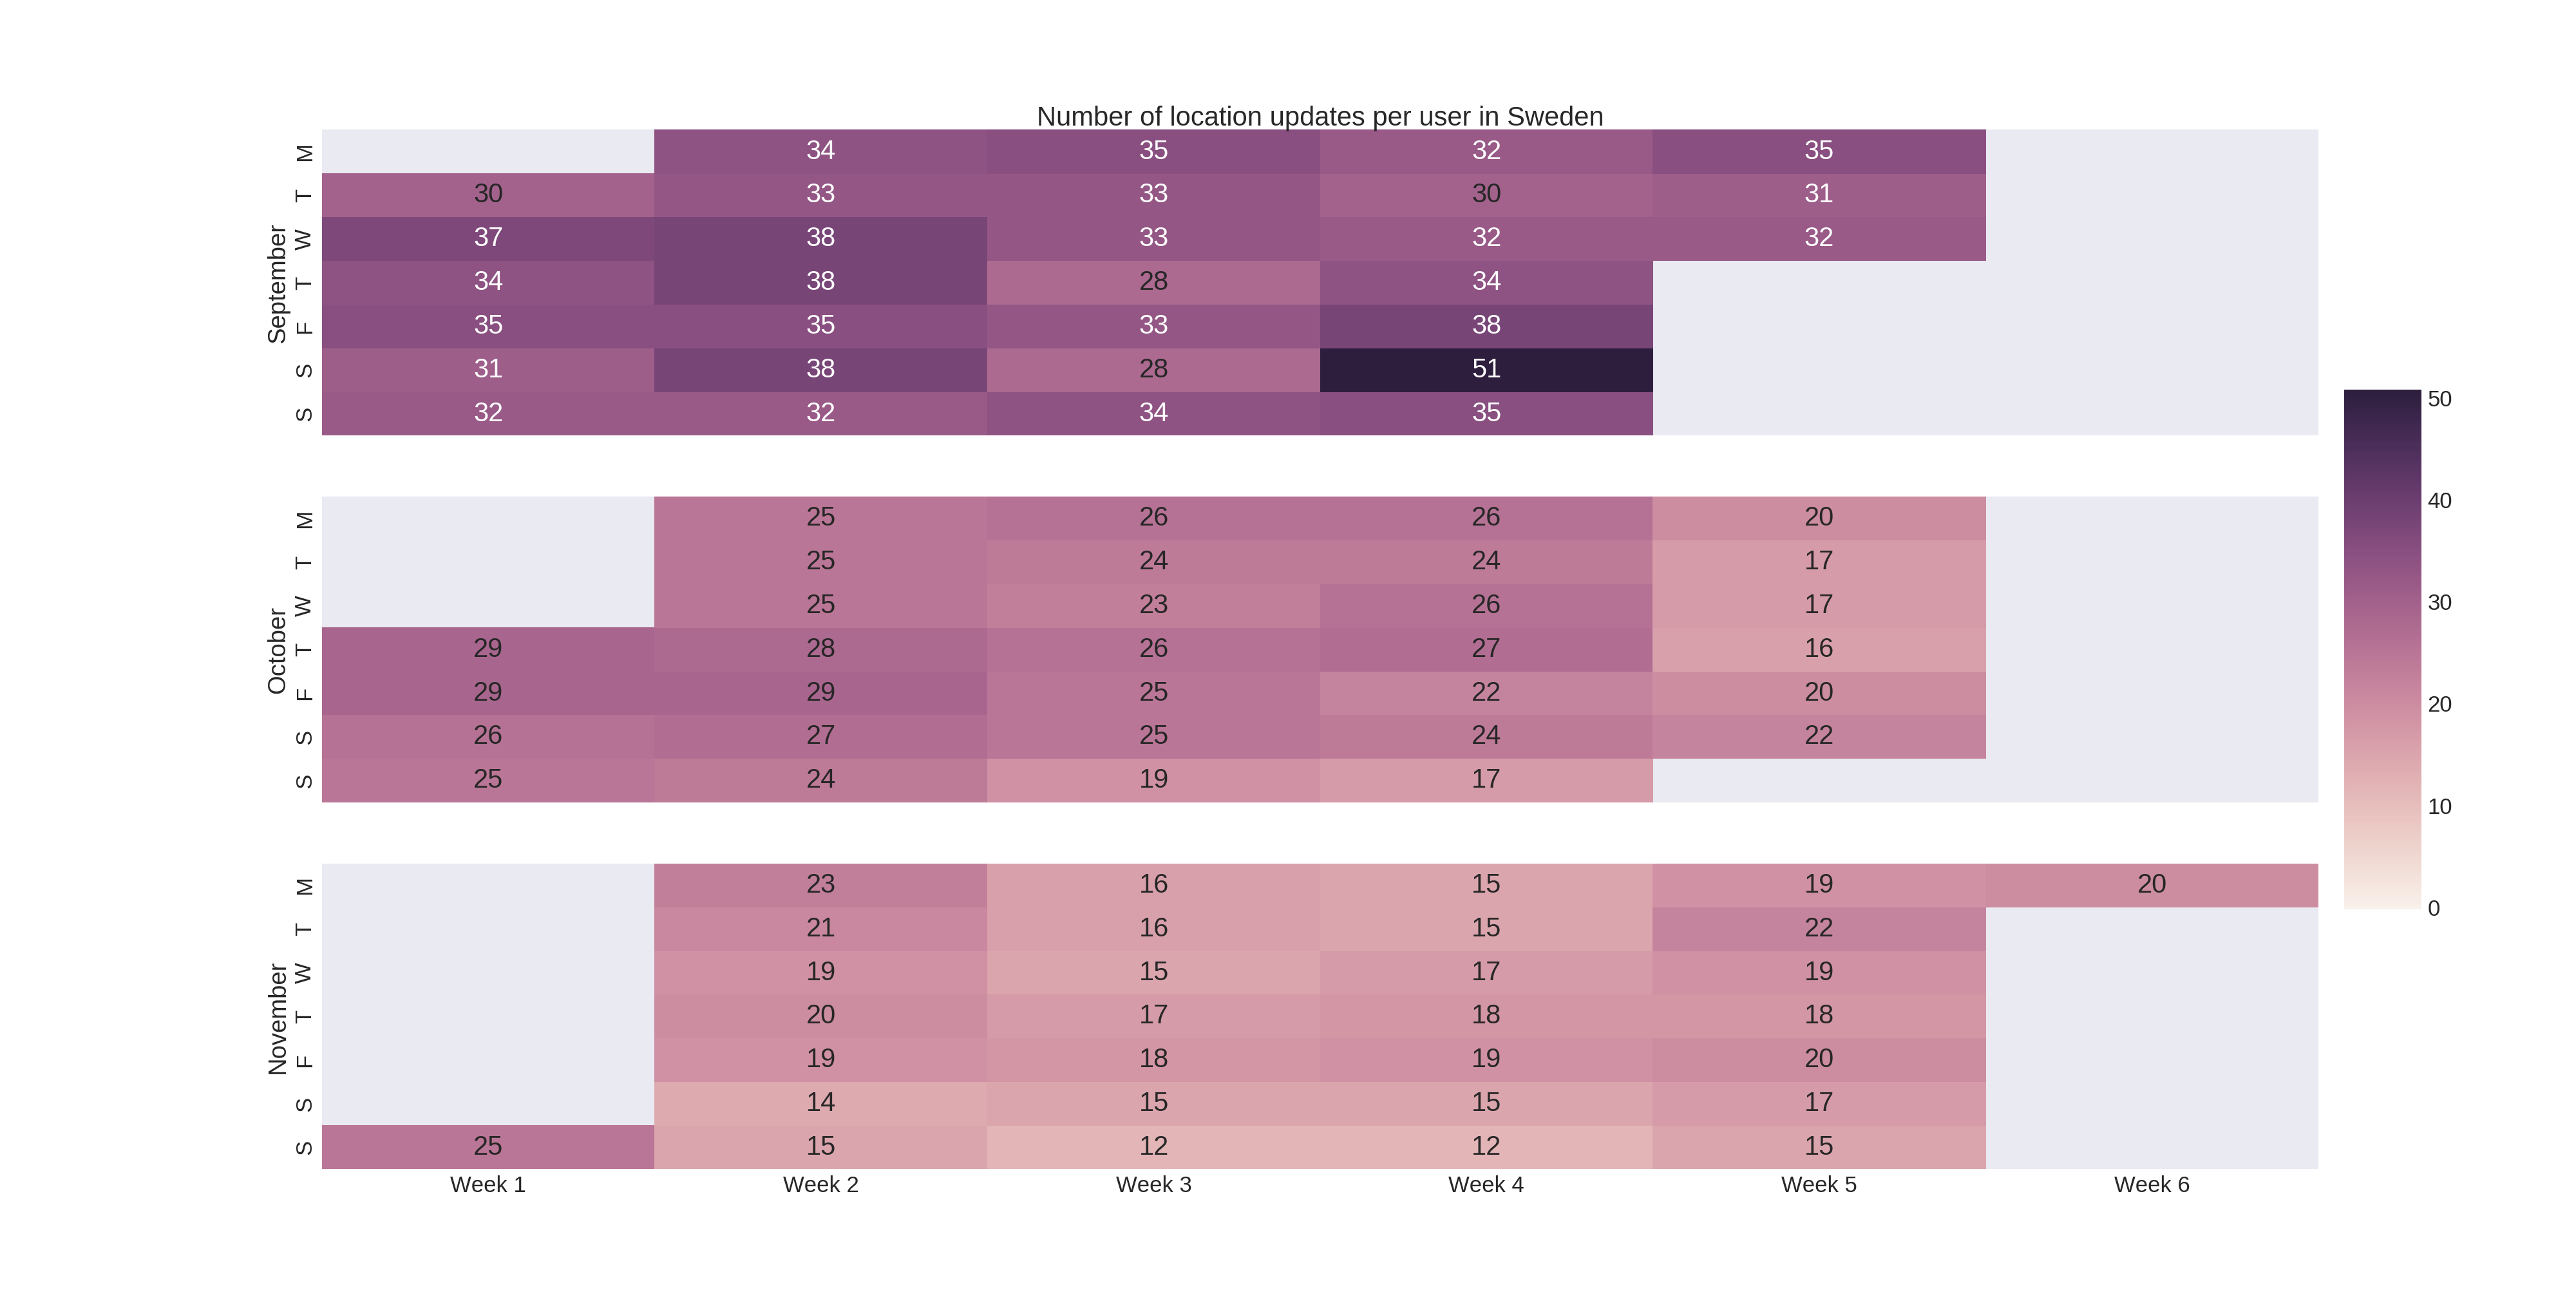
\includegraphics[scale=0.15]{heatmap_location_updates_sweden}
    \caption{Heat map for mean location updates over the 3 month period in Sweden}
    \label{fig:heatmap_swe}
\end{figure}

Figure \ref{fig:heatmap_swe} shows how location updates per user in Sweden (rounded to nearest integer) is distributed for each day in each of the three months. As in Japan we have in general more updates in September than in the other two months. In Sweden this tendency is more pronounced than in Japan. As in Japan this tendency has been observed in Figure \ref{fig:mean_loc_updates_sep-nov}, so it is not surprising.  
 
Here too, like in Japan, the values for Fridays and/or Saturdays are slightly higher than for the other days. The values are not so much higher that it is of importance, which is also the case for Japan. 

In the two figures above, we can get a feeling for the mean number of updates for each day. It is not possible to get a feeling for the situation for each user. Because of this the following figures have been produced. 

\begin{figure}[H]
    \hspace*{-1.5cm}
    \centering
    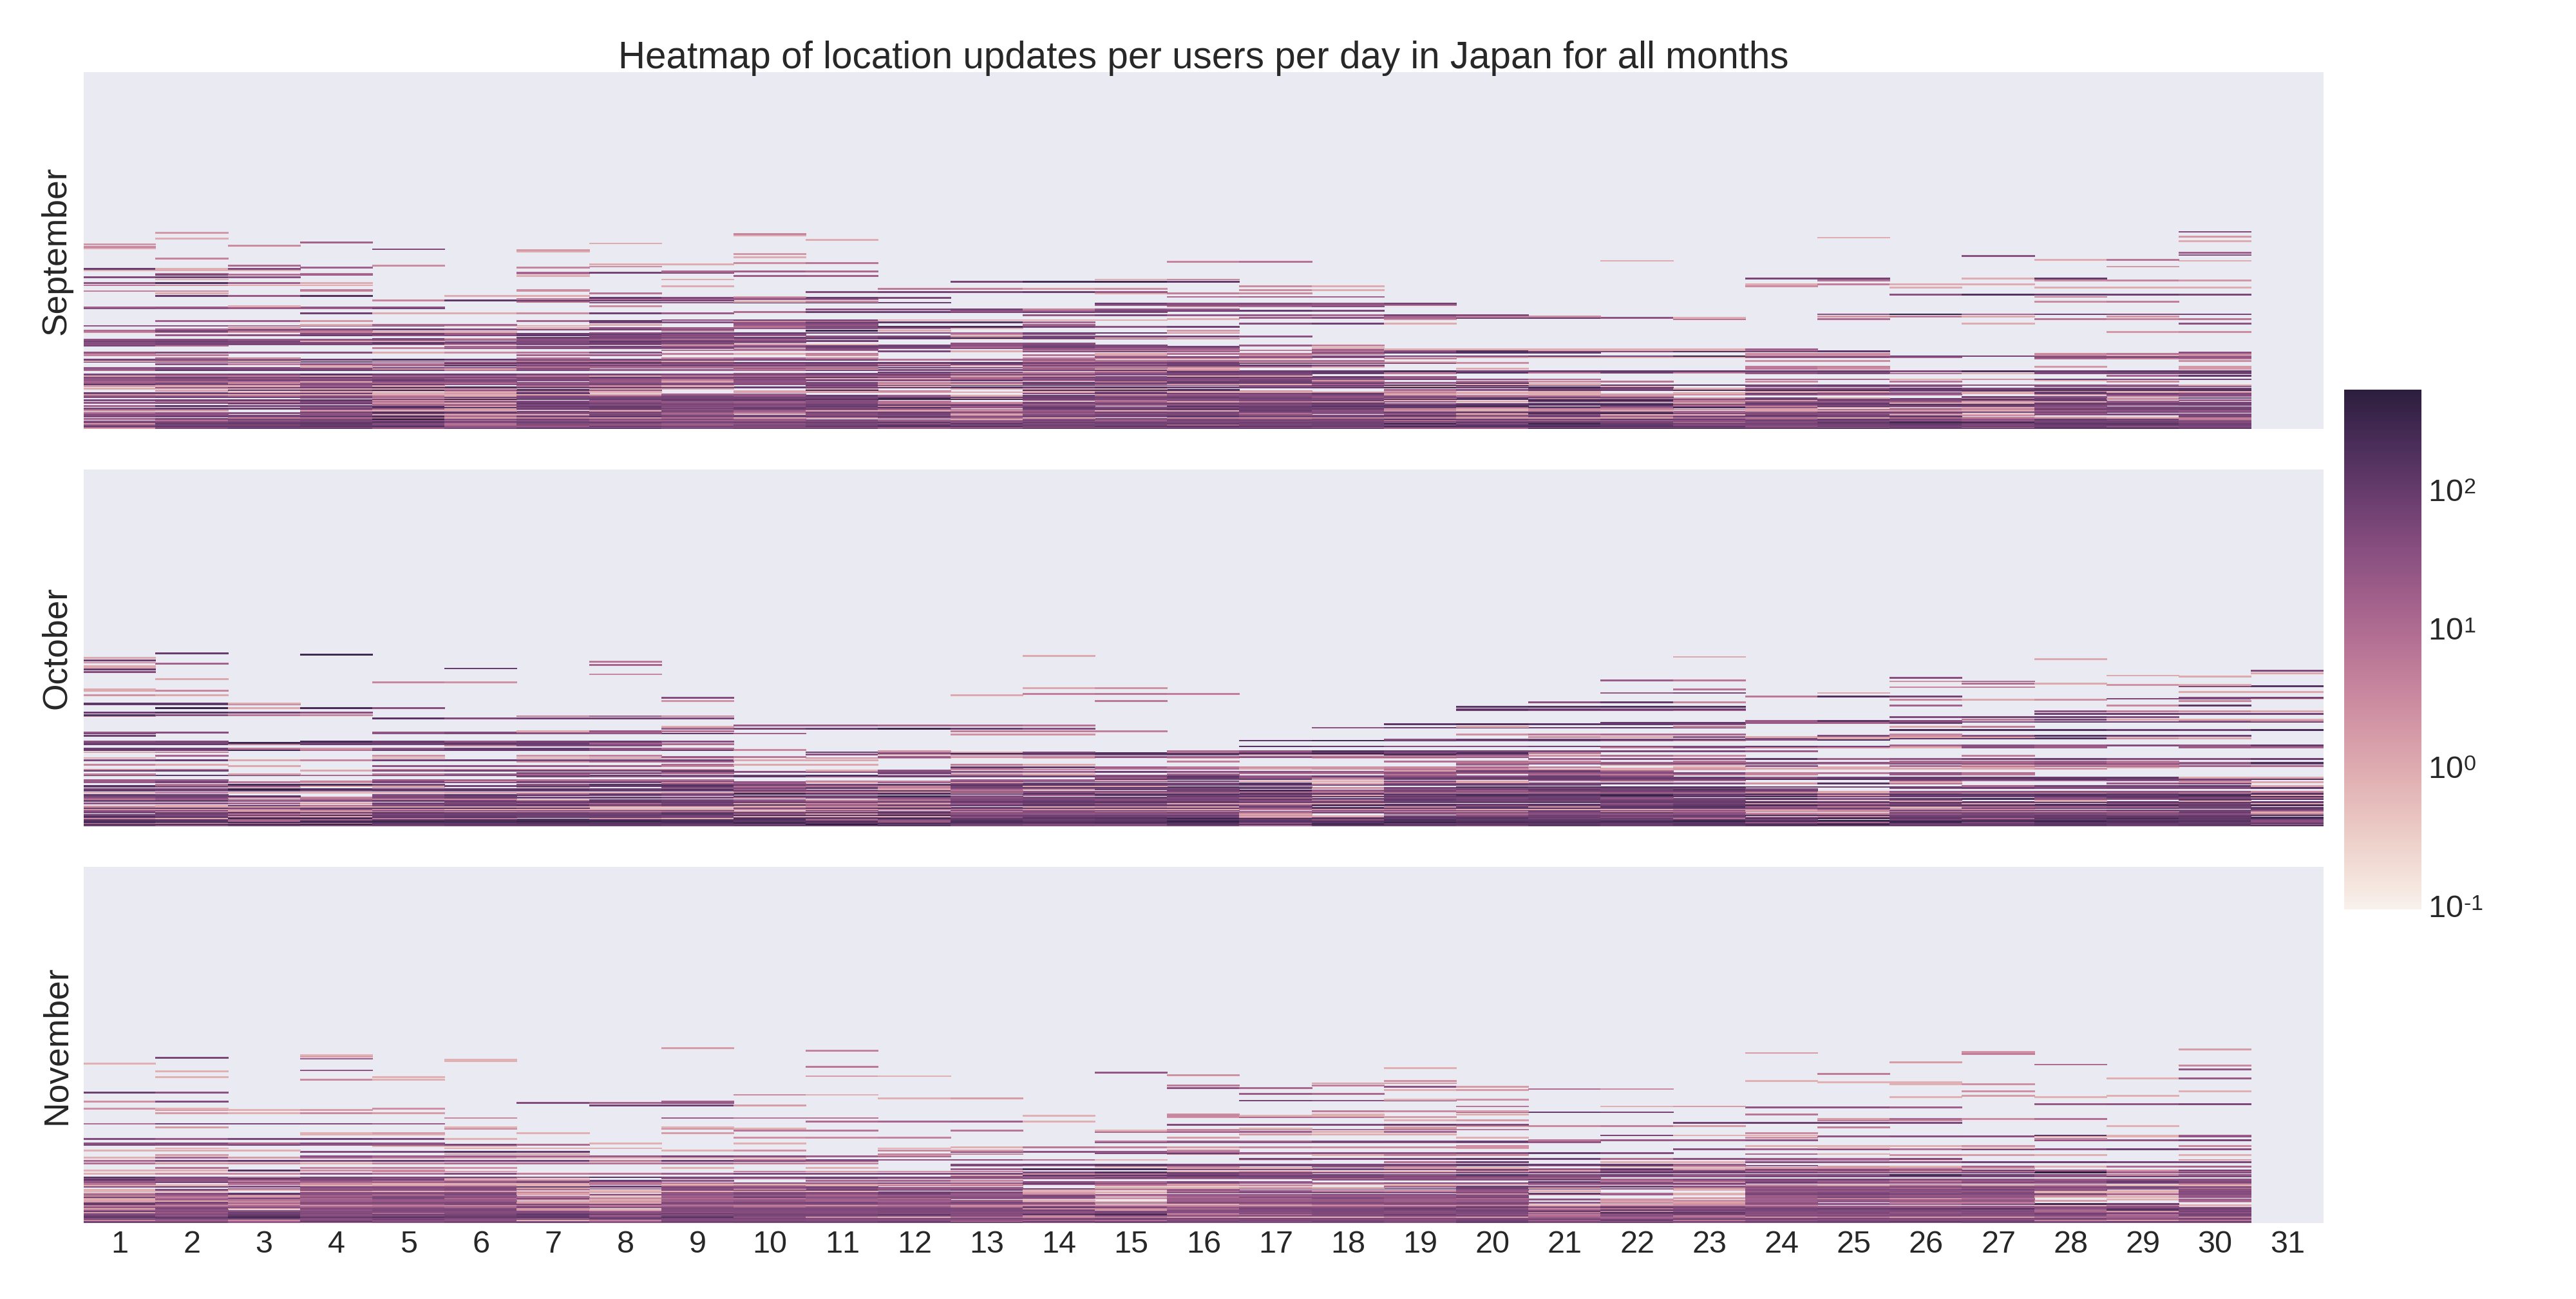
\includegraphics[scale=0.16]{location_updates_japan_combined_log.png}
    \caption{Heat map for mean location updates over the 3 month period in Japan. x-axis is days and y-axis is users. The scale is logarithmic}
    %\vspace*{-3.5cm}
    \vspace{-12pt}
    \label{fig:heatmap_japan_combined}
\end{figure}
Figure \ref{fig:heatmap_japan_combined} shows the number of updates for each user (y-axis) for each day in each of the three months (x-axis). Each row in each of the three heat maps (one for each month) represents one user. So there are \numberUsersJapan{} number of rows in each heat map.  Each heat map is sorted so the user with most updates in most days is in the lowest row. This means that the users are not necessarily represented in the same row in all three heat maps. It can also be seen that many users (approximately half) has no updates in some of the days for each of the three months. This is reasonable from what is known from Figure \ref{fig:country_cdf} and these users are as mentioned not necessarily the same over all the months. 
The days and months are plotted this way as it gives a possibility to compare the days for each month with each other. 

It can be seen that there are relatively few users who has updates in all days in a month. This fact alone is worrying and does not look promising for the thesis, and when we in this plot cannot be sure that it is the same user that has updates in all days in the three months, it looks even more worrying. 

Again it seems that September has more users who have updates in relatively more days than in the other months. 

If we look at October, we can see some pairs of days which make light vertical stripes in comparison with the other days. This indicates a lower amount of updates. This is happening  on the 3rd and 4th, 10th and 11th, 17th and 18th and at last the 24th and 25th. These pairs pop up with an interval of a week, where the 3rd is a Saturday and the 4th is a Sunday. This means that the other pairs are also Saturdays and Sundays. This pattern is repeated in November where it is really significant on the 7th and 8th. The data for September are not so distinct but the effect is observable. This is very interesting as it may indicate that Saturdays and Sundays are not suited for the purpose. 

Otherwise no days or periods stands out from the main data. The reason that the 31st September and November are empty is that these dates are invalid, while the 31st of October exists. Therefore the dates for September and November must be empty.  

\begin{figure}[H]
    \hspace*{-1.5cm}
    \centering
    
\includegraphics[scale=0.16]{location_updates_sweden_combined_log.png}
    \caption{Heat map for mean location updates over the 3 month period in Sweden. x-axis is days and y-axis is users. The scale is logarithmic}
    \label{fig:heatmap_sweden_combined}
\end{figure}
Figure \ref{fig:heatmap_sweden_combined} shows the same for Sweden. Again it can be seen that Saturdays and Sundays deviates from the other days by having fewer updates. It can also be seen that September has fewer users without updates during the month than Japan, where October and November is more similar in level to Japan. 

Sweden also has more users with updates every day than Japan. 

By using Figure \ref{fig:heatmap_japan_combined} and Figure \ref{fig:heatmap_sweden_combined} we can get a feeling for which days are better than others, e.g. that Saturdays and Sundays seems not so good as there are fewer updates. 

Otherwise no days or periods stands out from the main data. As for Japan the 31st September and 31st November are empty as these dates do not exist.  

One thing is to be able to see how the updates are distributed per day per user, but it is not known whether all the updates for a day occurs in one hour or whether they are distributed all over the day. We want to find users with a large number of location updates for each period as a higher opportunity for knowing where they went will result in a higher probability of knowing if they meet or not.  


\begin{figure}[H]
    \hspace*{-2.0cm}
    \centering
    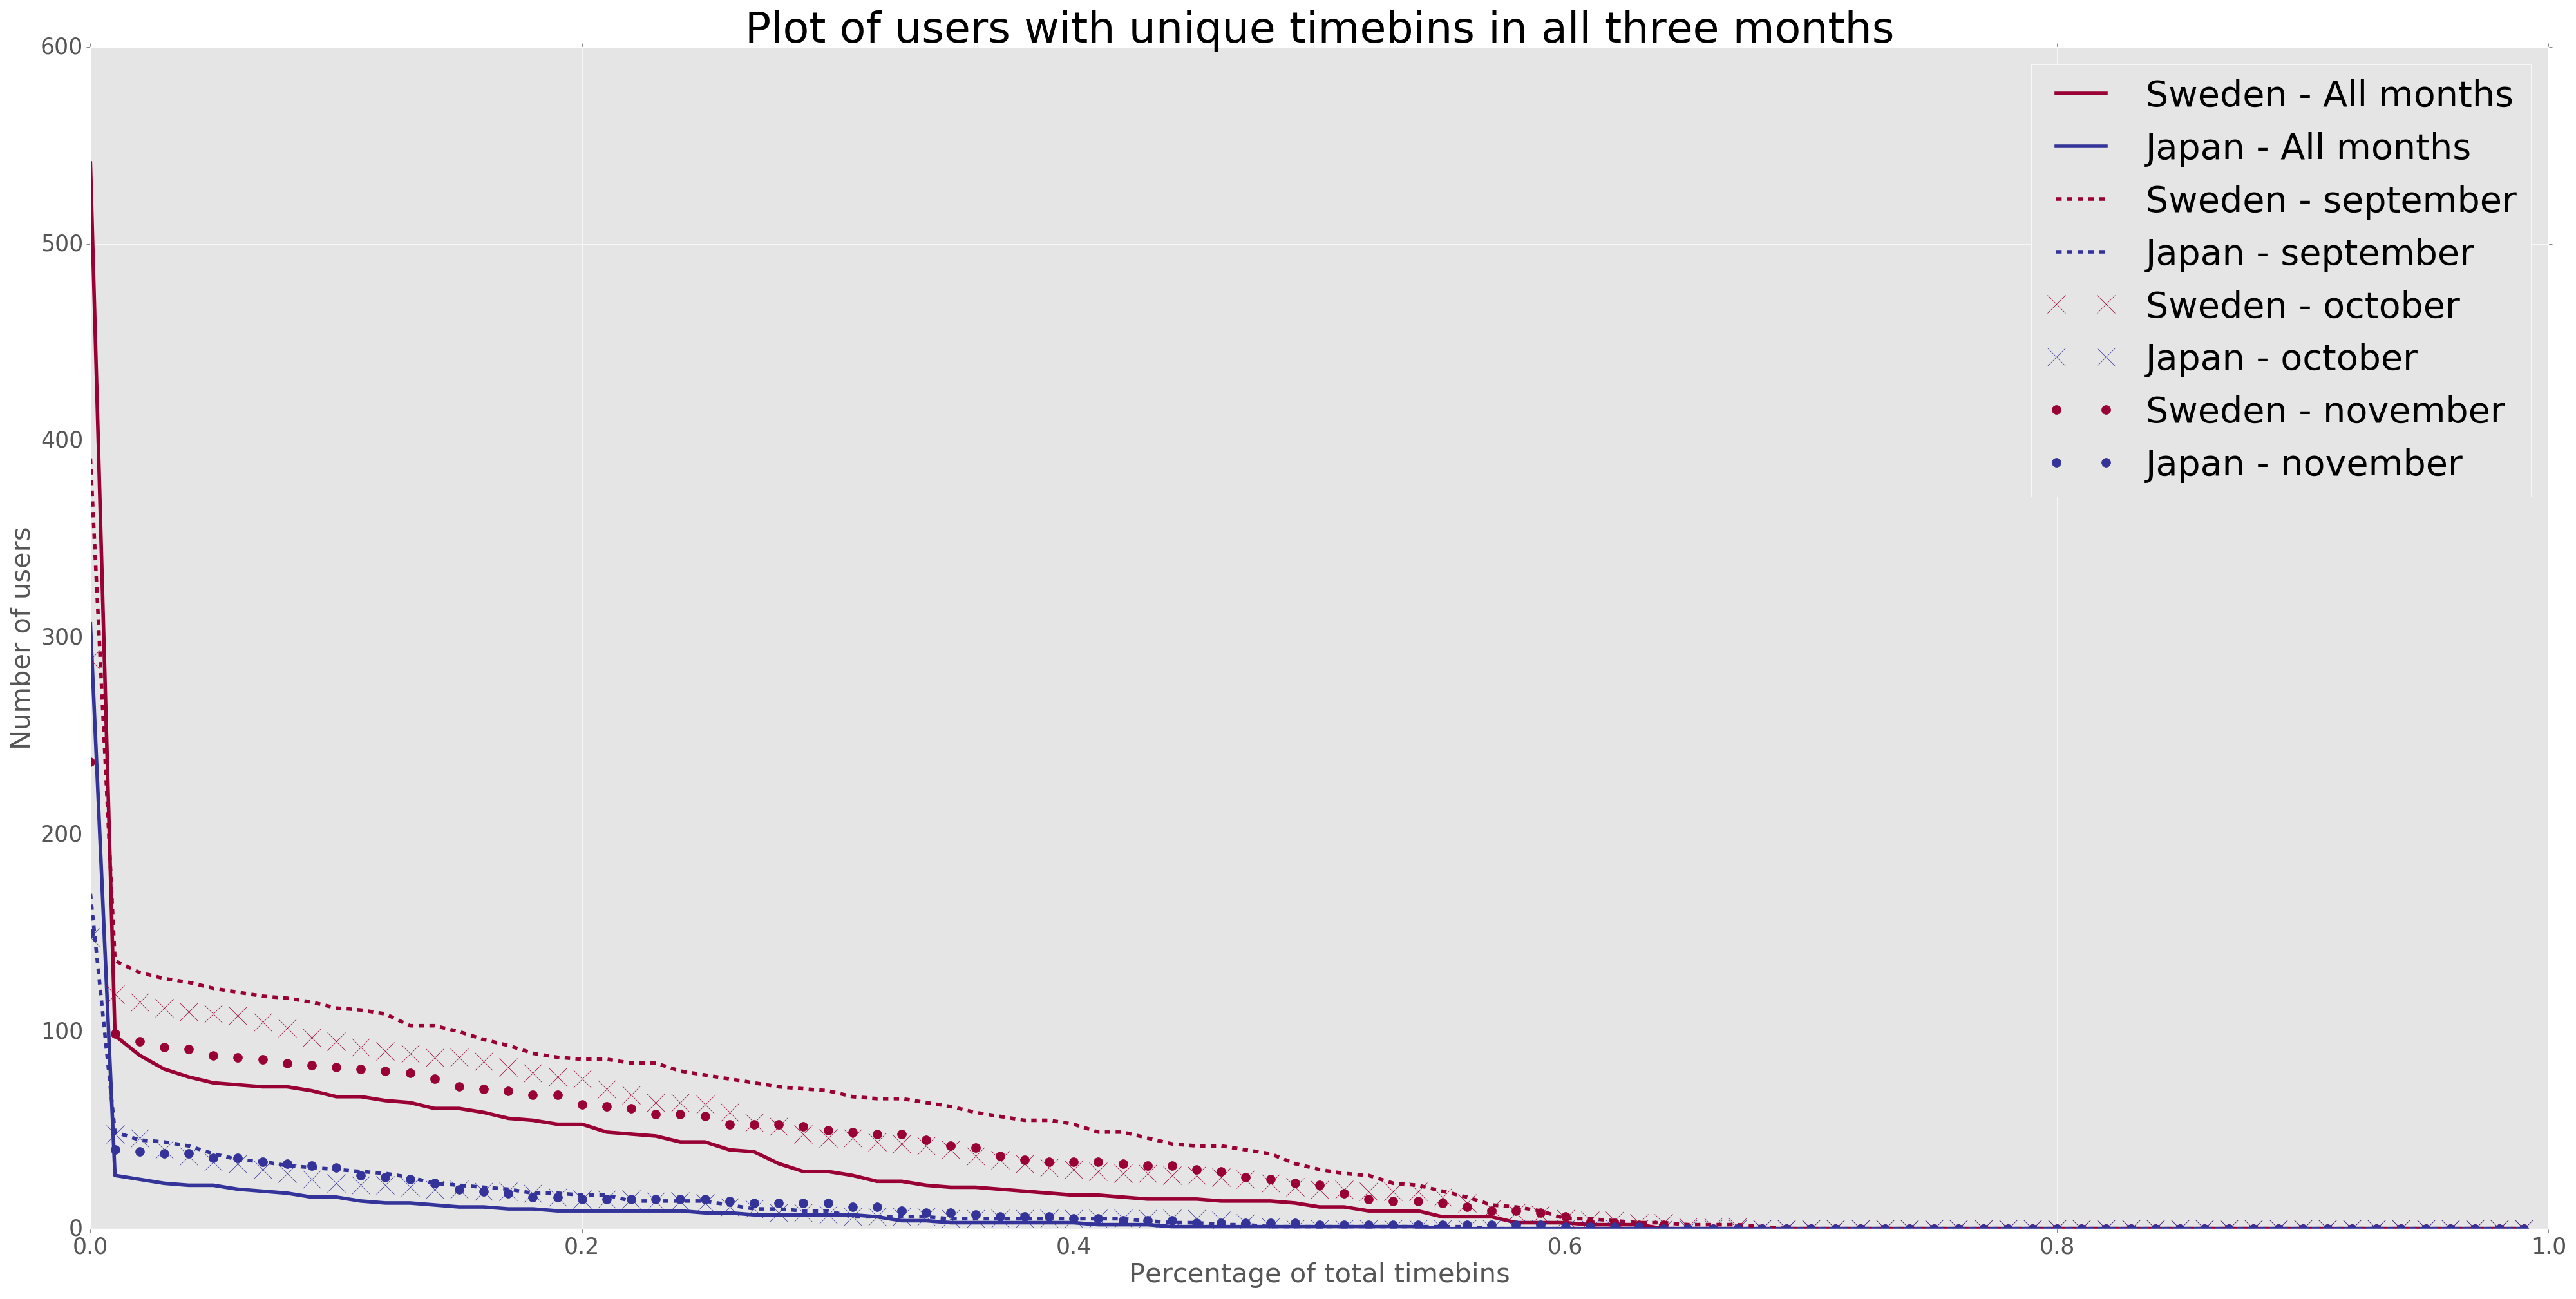
\includegraphics[scale=0.16]{users_by_criteria.png}
    \caption{Plot over number of users which have location updates in certain percentage unique time bins in each sub-period. A sub-period is defined in chapter \ref{chap:methods}, which is a period decided in three. In all month is a month a sub-period}
    \label{fig:users_by_criteria}
\end{figure}
From chapter \ref{chap:methods} it is known that the chosen period is divided into three sub-period to be able to train and analyze on these. Figure \ref{fig:users_by_criteria} shows how many users who has location updates in a certain percentage of unique time bins in all three sub-periods for a given period. For example we can see that there are approximately 90 users who have updates in 20\% of the possible time bins in each of the three sub-periods in Sweden in September. From now on we will use the term \textbf{cross-occupancy} when referring to the metric of users with a certain percentage of time-bins occupied in all three sub-periods, we thus have 90 users with 20\% cross-occupancy. Here the 30 days of September are divided into the following sub-periods: 1-10, 11-20, 21-30. 

It can be seen that a large amount of users have updates in very few time bins in each sub-period. The values are calculated with a resolution of 1\%. Already at 1\% unique time bins the number for September in Sweden has changed from \numberUsersSweden{} to approximately 140. This means that 140 users have updates distributed on 1\% of the possible time bins in each sub-period. For the other months the number is even lower. This is a very drastic decrease in the number of users. 
As a sub-period in September has 10 days and our time bins have a size of one hour, we have $10*24=240$ possible time bins. 1\% of this is equal to $240/100=2.4$, which means that the 140 users must have updates over 3 unique time bins in each of the three sub-periods, as we shall round to the next higher integer. 
The 90 users with 20\% cross-occupancy have updates over 48 unique time bins in each period. 

Using all months the sub-period is a month which is 30 - 31 days. 

In general we can see that even if the data development starts with a huge dip, it flattens out very quickly. September in Sweden is clearly better than the other months in Sweden, whereas in Japan the situation is less clear. Here it seems that the choice may be made between September and November. 



\subsection{App usage data}
In this section we will describe the app usage portion of the data from the test dataset.
The data spanned the same months as the test data and was in the same format.

The data contained the following attributes:
\begin{enumerate}
\item \texttt{\textbf{timestamp\_seen}}\\Milliseconds since the epoch showing when the app usage update is logged on the server/cluster 
\item \texttt{\textbf{id}}\\activity uuid represented as a string  
\item \texttt{\textbf{useruuid}}\\Unique user id represented as a string 
\item \texttt{\textbf{deleted\_time}}\\ If the activity has been deleted, this is the timestamp when it occurred, default is empty string
\item \texttt{\textbf{start\_time}}\\Time when the user enter an activity. Represented as an ISO8601 time stamp with time zone 
\item \texttt{\textbf{end\_time}}\\Time when the user leaves an activity. Represented as an ISO8601 time stamp with time zone
\item \texttt{\textbf{package\_name}}\\ The package name of the started activity
\item \texttt{\textbf{application\_name}}\\The human readable name of the started activity
\item \texttt{\textbf{category}}\\Name of the the category of the application as determined by Sony Lifelog
\item \texttt{\textbf{genre}}\\Name of the Google Play genre of the application
\item \texttt{\textbf{icon}}\\ An URL to the application icon image
\item \texttt{\textbf{devices}}\\The device is represented as an array with name, type and id. Type is the type of device (e.g. Phone), name is the name of the current device and the id is the unique identifier of the device 
\end{enumerate}
As can be seen from the attributes, the data contains information about which apps the users are using and when the app is in the foreground.

We used the data for implementing the App similarity measure as is described in Chapter \ref{chap:methods}.

\subsection{Demographics data}
In this section we will describe the demographics portion of the data from the test dataset.

The data consisted of a birthdates and genders for 1174 users.

The CSV file containing the data consisted of the following attributes:
\begin{enumerate}
\item \texttt{\textbf{useruuid}}\\Unique user id represented as a string
\item \texttt{\textbf{gender}}\\Gender of user represented as a string, "MALE" or "FEMALE"
\item \texttt{\textbf{birthdate}}\\Birthdate of user represented as string in format yyyy-mm-dd
\end{enumerate}
We decide to plot the distribution of the user ages, which can be seen in Figure \ref{fig:user_age_distribution}. We can immediately see a huge outlier in number of users around 35 years of age.

\begin{figure}[H]
    \hspace*{-1.5cm}
    \centering
    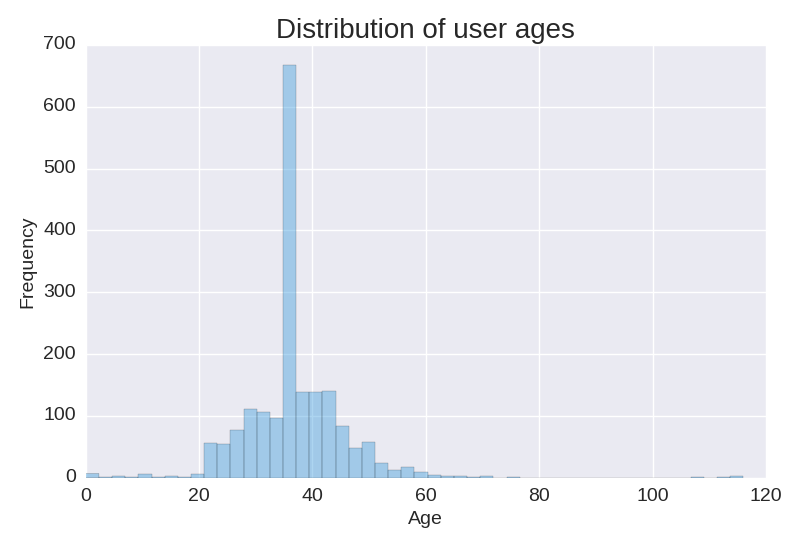
\includegraphics[scale=0.5]{user_age_distribution}
    \caption{The distribution of user ages}
    \label{fig:user_age_distribution}
\end{figure}
Looking closer at the data we can see the most frequent birthdates are December 1st, 1980, ('1980-12-01') for 346 users, January 1st, 1981, ('1981-01-01') for 86 users, the third most frequent is May 16th, 1976, ('1976'05-16') for 31 users.

We determine the two most frequent birthdates to be outliers as they occur on the first day of the month and are likely due to the users having accepted a default birthdate in the app as theirs. Removing the outliers we have a birthdate for the remaining 742 users.

We used the cleaned demographics data for implementing the homophily features described in Chapter \ref{chap:methods}.

When we first obtained the demographics data, we identified 5 users in our test datasets which were missing from the demographics data. 
We learned they were test-users, used for testing new features and thus we eliminated their location updates, 10 in total, from our datasets.

\section{Production data}
In this section we will describe the real-world production data from Sony servers.

Initially we tried using a newer month than the months from our test data, however we found the months did not have geocoding data (region, country, area, place) and thus we could not filter by country. An option would be to do reverse geocoding on the data. Another option would be a coarse filtration where we use the borders of Sweden in terms of latitude and longitude. Both of these options would take time. Instead we found the newest month folders with geocoding data intact was 09-15, 10-15, 11-15, the same months we had as test data, and we decided to use September as we have for the test data.

We found the data folder for 09-15 had 929,697,167 location updates. After our filtration by Sweden, accuracy and just the period of September we found a remaining number of location updates of 2,450,205 and number of users of 12,692.

We divided September into three periods, 1-10, 11-20, and 21-30 and extracted two datasets, one using all users and another using only the users with a certain cross-occupancy threshold. Using a cross-occupancy threshold of 40\% we found 296 users in period 1, 457 users in period 2, and 12561 users in period 3.

As we can see there is a very large influx of users in period 3, this could perhaps be due to a new version of Sony Lifelog released in that exact period, this could also mean the number of 12,692 users could in reality be much lower in the first two periods. Of the users in each period we found none with 40\% in all three periods, thus we picked a lower threshold of 10\%.




\section{Summary}
In this section we will present the most important findings in the analysis above. 

We have found that Sweden and Japan were the two countries with the largest representation of number of location updates.  On this basis we proceeded with the two countries, where we found that there were some data with values for accuracy which were invalid. These data were removed as these updates could not be trusted. Furthermore the data with an accuracy value of more than 50.000 were removed because of the binning size. 
The data were cleaned further by updating the 500.000 location updates where the country attribute were missing. On basis of the geolocation the relevant country could be identified, which increased the number of represented countries. But after all Sweden and Japan were the countries with most data represented. 

We found a decreasing tendency in the number of updates between the months where September had the most updates, where after the number decreased in the two following months. Of all the updates 23.89\% and 19.86\% respectively in Sweden and Japan occurred on Sony locations.  

When we looked at the \numberUsersSweden{} and \numberUsersJapan{} users in Sweden and Japan respectively, many had very few updates over all three months. It is assumed that many turned their phone off in the period 02:00 AM to 06:00 AM which leads to the few updates. This was valid for both Sweden and Japan. Furthermore it can be seen that the number of updates peaks at 08:00 AM and 04:00 PM in Sweden, where the number in Japan only peaks at 08:00 AM.  Japan has no corresponding peak at 04:00 PM. 

At last we found that in general there were not as many updates Saturdays and Sundays as for the other days. We also found that when we looked upon how many users who had updates over several time bins in each sub-period (called cross-occupancy), the number of users decreased very rapidly as a function of the number of time bins until a certain number. After this the decrease was very slow. In Sweden for September there were approximately 140 users having updates over 3 time bins in each sub-period, corresponding to 1\% of the possible time bins in each sub-period. If we looked at the number for 20\% (48 time bins in each sub-period) there were approximately 90  users. 

On the basis of this it seems that the data for Sweden in September looks most promising, and we will use them in our models. 
\newpage
%!TEX root = main.tex
\chapter{Methods and results}
\label{chap:methods_and_results}
In this section we will outline what methods we have used for conducting the work.
\section{Data preparation}

When we got the dataset it was stored in three folders, one for each month (9, 10, 11) and within each folder were multiple chunks of data in Apache Avro format\cite{apacheavro}, which we learned is a data serialization framework for Hadoop similar to the JSON format. The chunks were contained in folders bearing the number for each month, however we learned they were sorted by when the server had received the data packet containing the location from the phone and not when the phone had registered the location. The app is storing the collected data on the users phone for a maximum of one month, if the data is not uploaded within a month it is discarded. This approach to data collection means the month folders can contain location updates from the previous month as well.


\subsection{Data import to database}
We imported the many JSON files to a Postgresql database which allowed us to easily manipulate the data using SQL. We created a single table with the schema shown in Table \ref{table:schema_denormalized}. We decided to compute the time and spatial bins on insertion, thus we only had to compute them once. We created indexes on the following features:start\_time, end\_time, location, useruuid, spatial\_bin, time\_bins, country.
Initially we created a normalized database with several relations. We however discovered that a deonormalized database might improve our performance, as we reduce the number of tables and and thus the number of joins required\cite{sanders2001denormalization}. We found This was due to all our interaction with the data only consisting of READs, after the initial insertion of the data. After removing all relations (denormalizing) our performance significantly improved.

\begin{table}[htbp]
\centering

\begin{tabular}{|c|c|c|c|c|c|c|c|c|c|c|}
\hline
\textbf{Field name} & \textbf{Field type}    \\
\hline
id                  & SERIAL PRIMARY KEY     \\
\hline
useruuid            & TEXT NOT NULL          \\
\hline
start\_time         & TIMESTAMPTZ NOT NULL   \\
\hline
end\_time           & TIMESTAMPTZ NOT NULL   \\
\hline
location            & GEOGRAPHY(POINT, 4326) \\
\hline
altitude            & INTEGER NOT NULL       \\
\hline
accuracy            & INTEGER NOT NULL       \\
\hline
region              & TEXT                   \\
\hline
country             & TEXT                   \\
\hline
area                & TEXT                   \\
\hline
place               & TEXT                   \\
\hline
time\_bins          & INTEGER{[}{]} NOT NULL \\
\hline
spatial\_bin        & BIGINT NOT NULL        \\
\hline
\end{tabular}
\caption{Denormalized database schema}
\label{table:schema_denormalized}
\end{table}
\subsection{Data export to Numpy arrays}
We created scripts for exportation to numpy arrays for use in the sklearn module. The users were encoded with K values where K = number of users. The countries were encoded with K values where K = number of countries.

\subsubsection{Binning} \label{ssec:binning}
In the following section the term grid cell or spatial bin will be used synonymously, the same holds for time interval and time bin.
A spatiotemporal co-occurrence between two users is defined as an instance in which they co-occurred in approximately the same time and approximately the same place.
We have partitioned or binned the globe into a discrete grid where the cells span .001{\degree} of latitude and longitude on each side (approximately 111m at the equator), and in a discrete time interval of 1-hour.
Thus we say a co-occurrence happens between users $i$ and $j$ if they share the same .001{\degree} spatial cell C within the same discrete time interval.

Each grid cell has a unique ID, this is obtained by considering the grid as a matrix and flattening it to a list by traversing from left to right and top to bottom (row-first ordering) and using the list index as an ID. This makes a total possible spatial bin indexes of: $$(190\times d)\times(360\times d)$$ where $d$ is the number of decimals, this makes in our case a total number of spatial bins of $68.400.000.000$ with our case of $d=3$.

We calculated the time bins by counting every hour from the start of the day of the earliest date appearing in the dataset, which has the ISO 8601 timestring: "2015-08-09 22:25:33.766+02". The last day has the ISO 8601 timestring: "2015-12-01 00:59:15.738+01". This leaves us with $2738$ possible time bin IDs. As each location update has a start\_time and an end\_time, each update will result in one or more entries for each time bin. For generating our dataset we count co-occurrences between pairs only once per spatial and time bin.
\begin{figure}[H]
    \hspace*{-1.0cm}
    \centering
    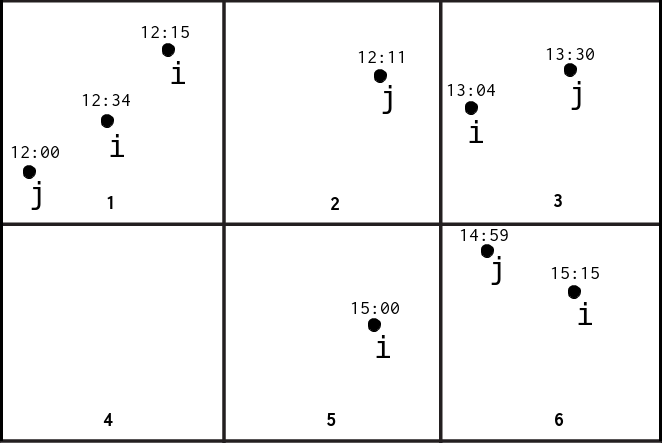
\includegraphics[scale=0.30]{grid}
    \caption{Illustration of spatiotemporal co-occurrences, users $i$ and $j$ have 2 co-occurrences in spatial bin 1 and 3, spatial bin 6 have different time bins.}
    \label{fig:binning}
\end{figure}

\subsection{Visualization}
We used Basemap\cite{basemap}, for plotting all the locations at once and and Leaflet\cite{leaflet} for producing interactive maps to visualize the data, we created a map for visualizing the users location traces over time and we created one that allowed us to see all the co-occurrences that happened between a pair of users. Figure \ref{fig:sweden_locations_hexbin} and \ref{fig:japan_locations_hexbin} shows location updates from Sweden and Japan respectively plotted on a map. We can see location updates happened very often near Sony properties in Lund\cite{sony_headquarters_sweden_lund}, Kista\cite{sony_headquarters_sweden_kista}, and at Ericsson AB in Göteborg\cite{ericsson} for the Swedish data, and in Tokyo\cite{sony_headquarters_japan} for the Japanese data. Figure \ref{fig:user_pair_at_sony} shows an example of the co-occurrences visualized for a typical pair of users in Sweden having lots of co-occurrences within the Sony perimeter. This enabled us to exclude co-occurrences from these locations from our dataset as we are looking for co-occurrences outside of the users work.
\begin{figure}[H]
    \hspace*{-1.0cm}
    \centering
    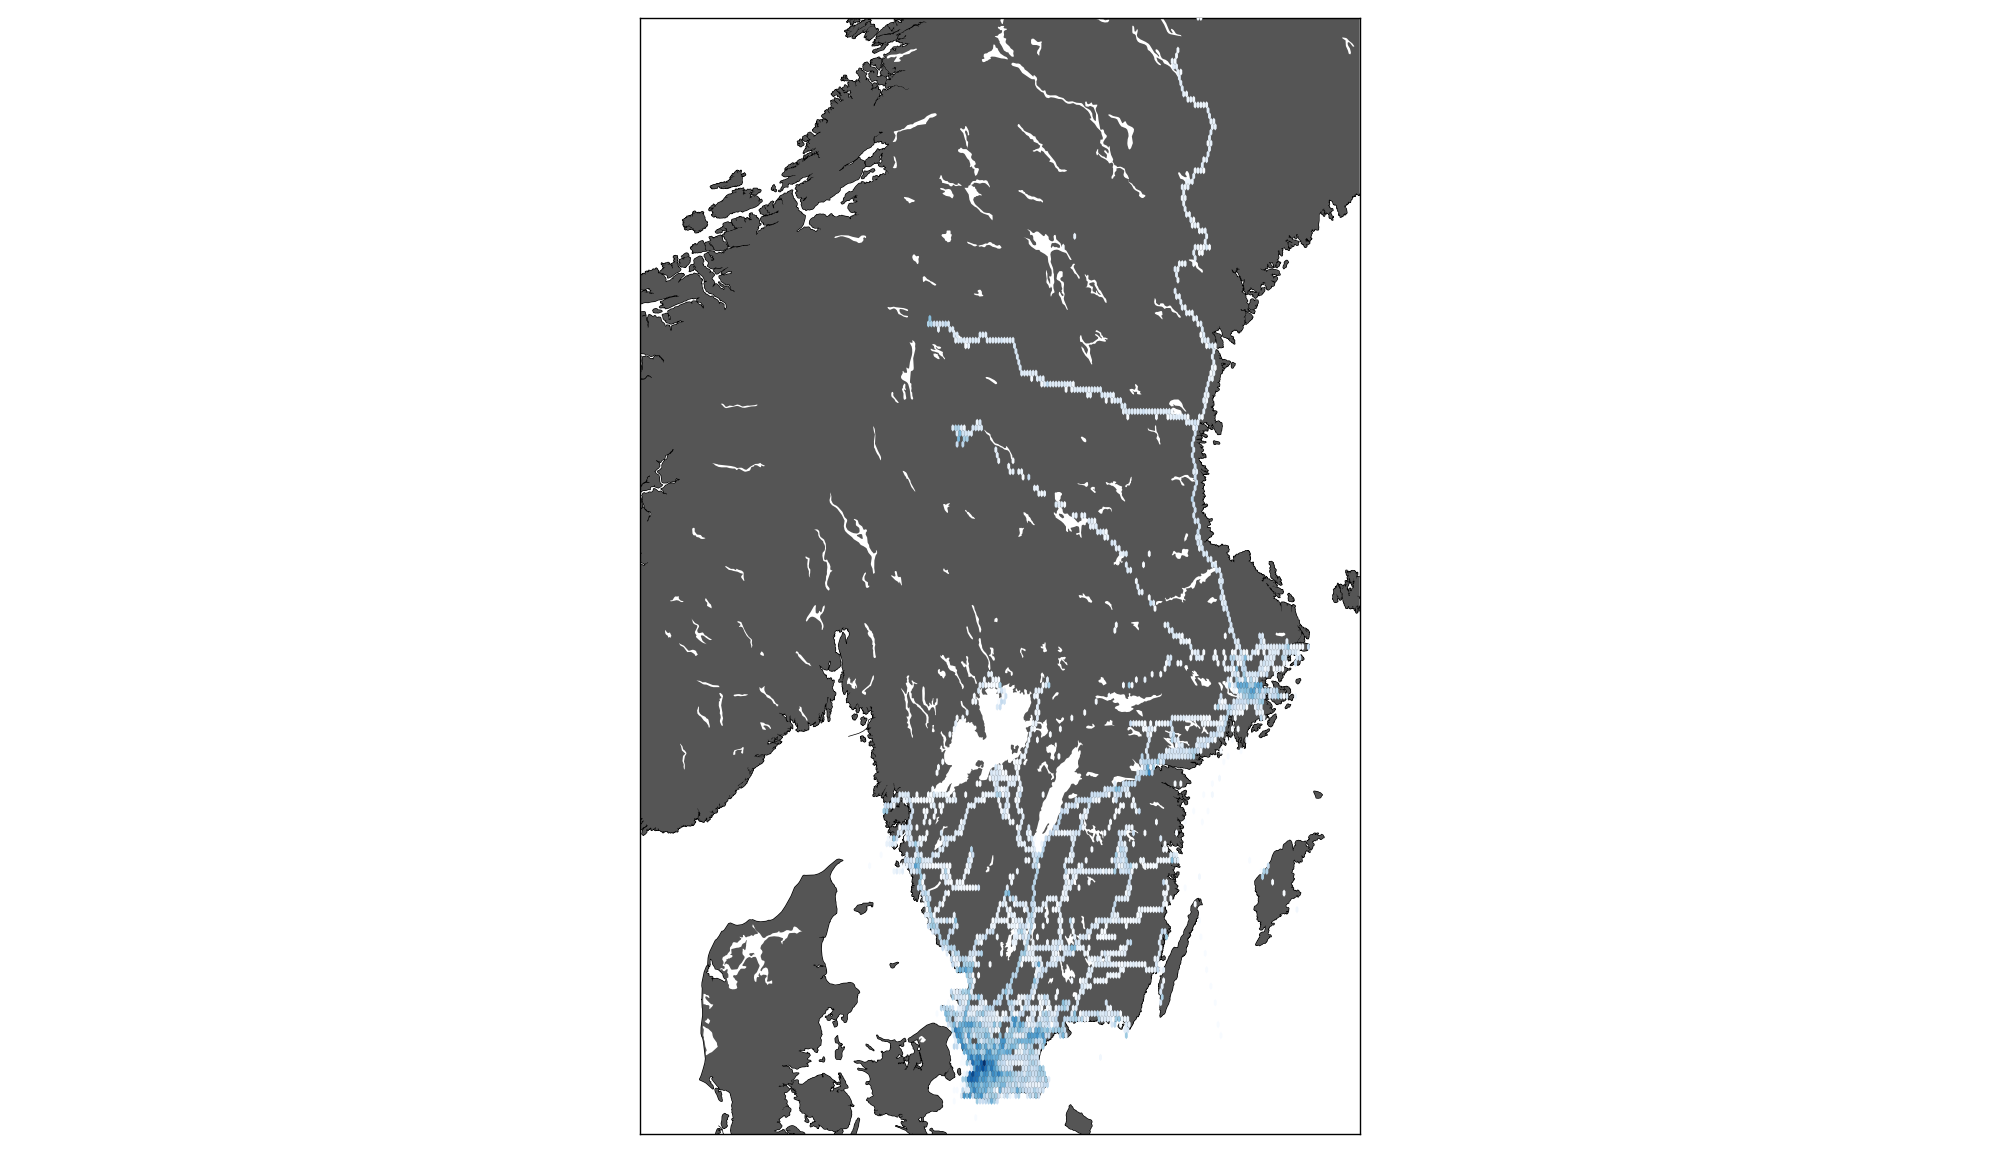
\includegraphics[scale=0.30]{all_locations_sweden}
    \caption{Location updates in Sweden, hex-binned in log scale}
    \label{fig:sweden_locations_hexbin}
\end{figure}
\begin{figure}[H]
    \hspace*{-1.0cm}
    \centering
    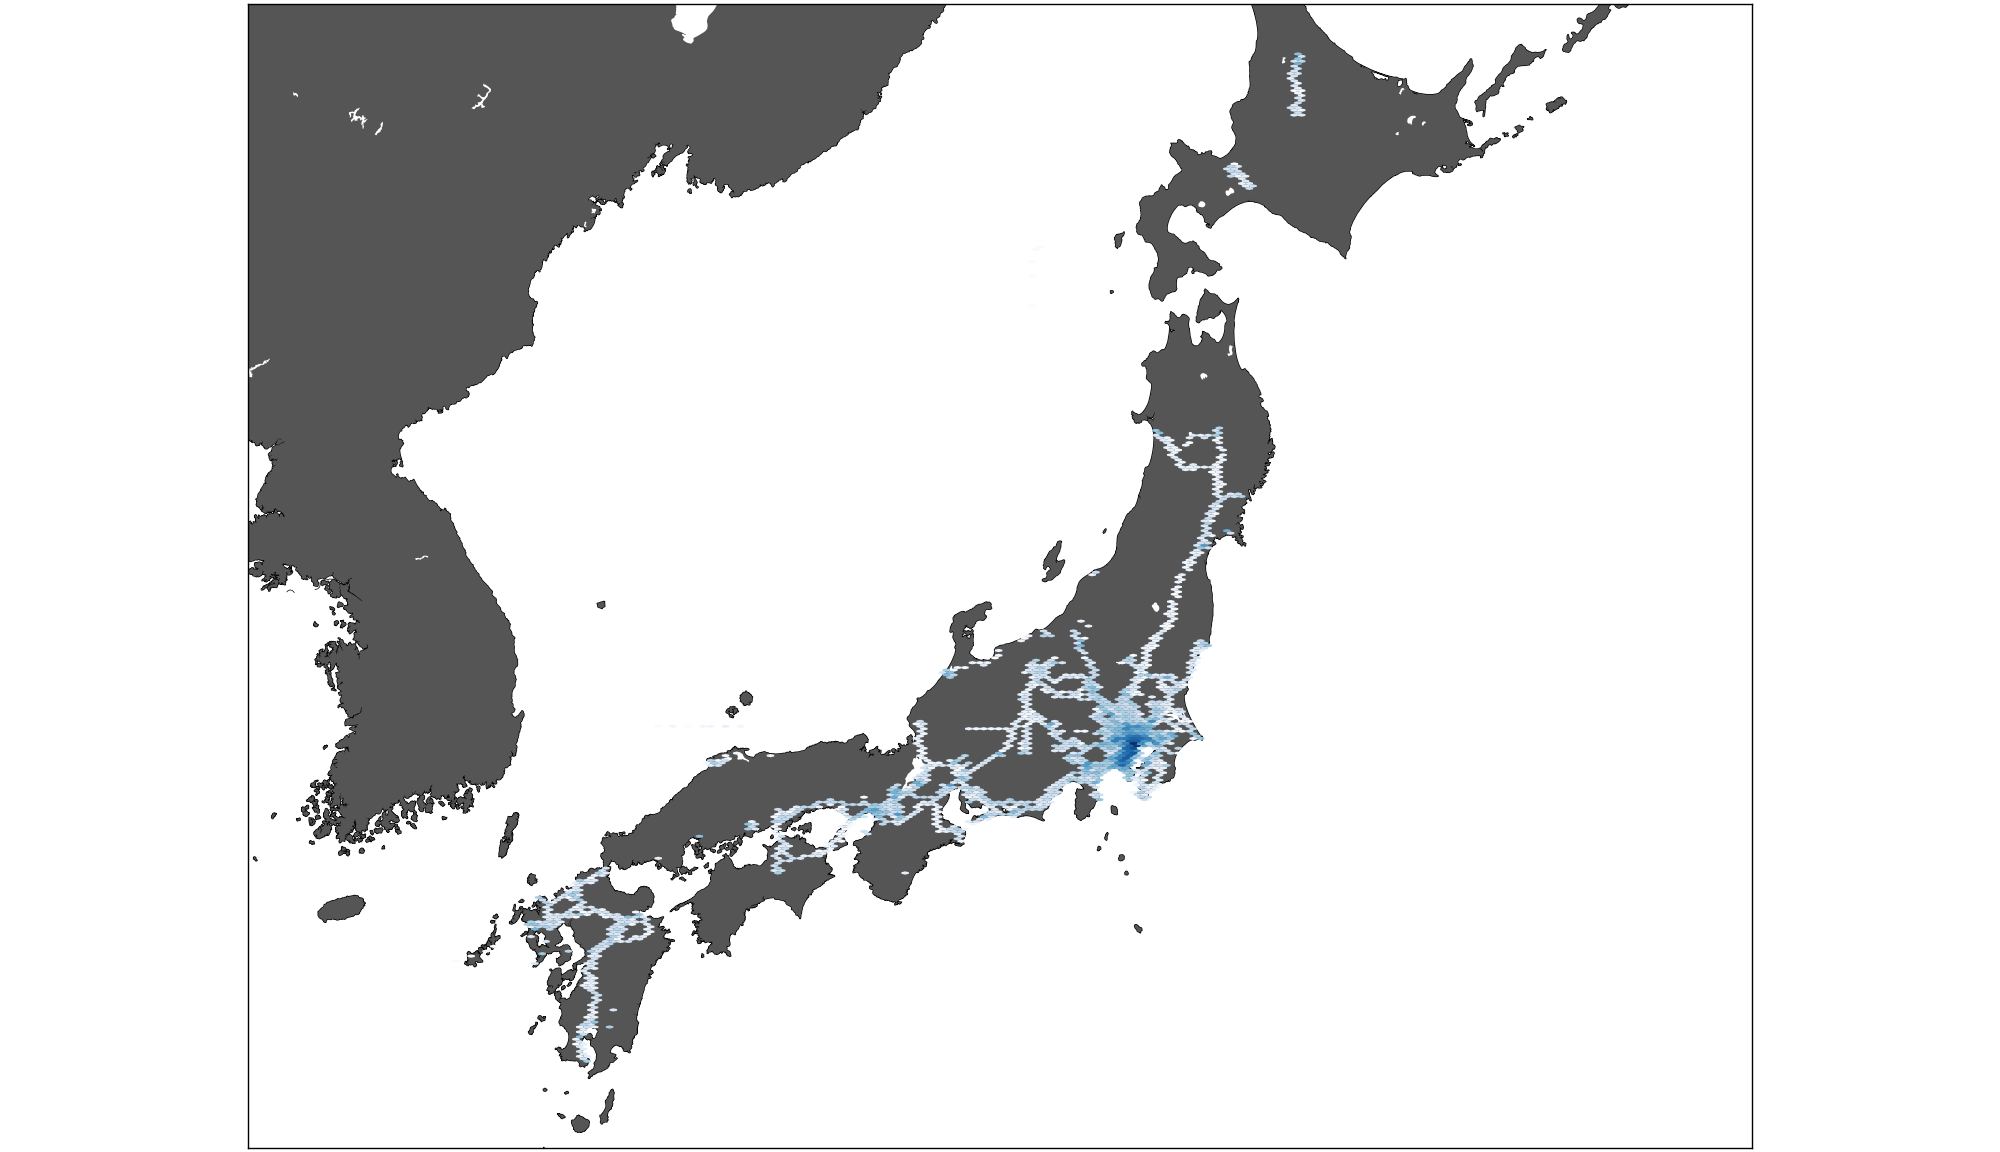
\includegraphics[scale=0.30]{all_locations_japan}
    \caption{Location updates in Japan, hex-binned in log scale}
    \label{fig:japan_locations_hexbin}
\end{figure}
\begin{figure}[H]
    \hspace*{-1.0cm}
    \centering
    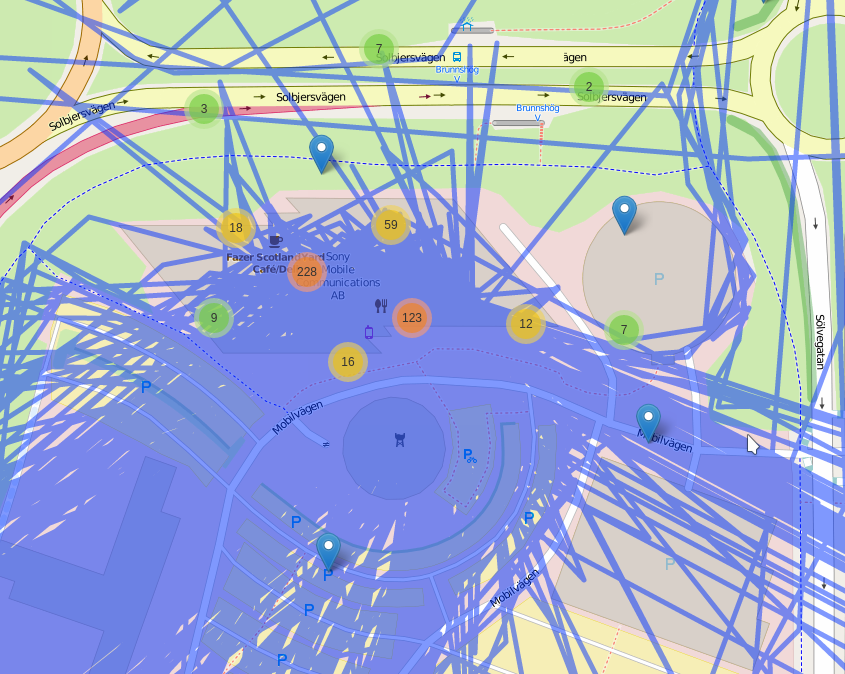
\includegraphics[scale=0.50]{user_pair_at_sony}
    \caption{User pair with high number of co-occurrences for whole period at Sony perimeters}
    \label{fig:user_pair_at_sony}
\end{figure}

We decided to look at just how many co-occurrences happened inside the Sony perimeter. Figure \ref{fig:dist_coocs_sony} shows the number of co-occurrences inside and outside Sony perimeters, here we see a massive amount of co-occurrences happening inside the Sony perimeters. This can pose a problem as we will only be looking at co-occurrences between users that is outside Sony perimeters.

\begin{figure}[H]
    \hspace*{-1.0cm}
    \centering
    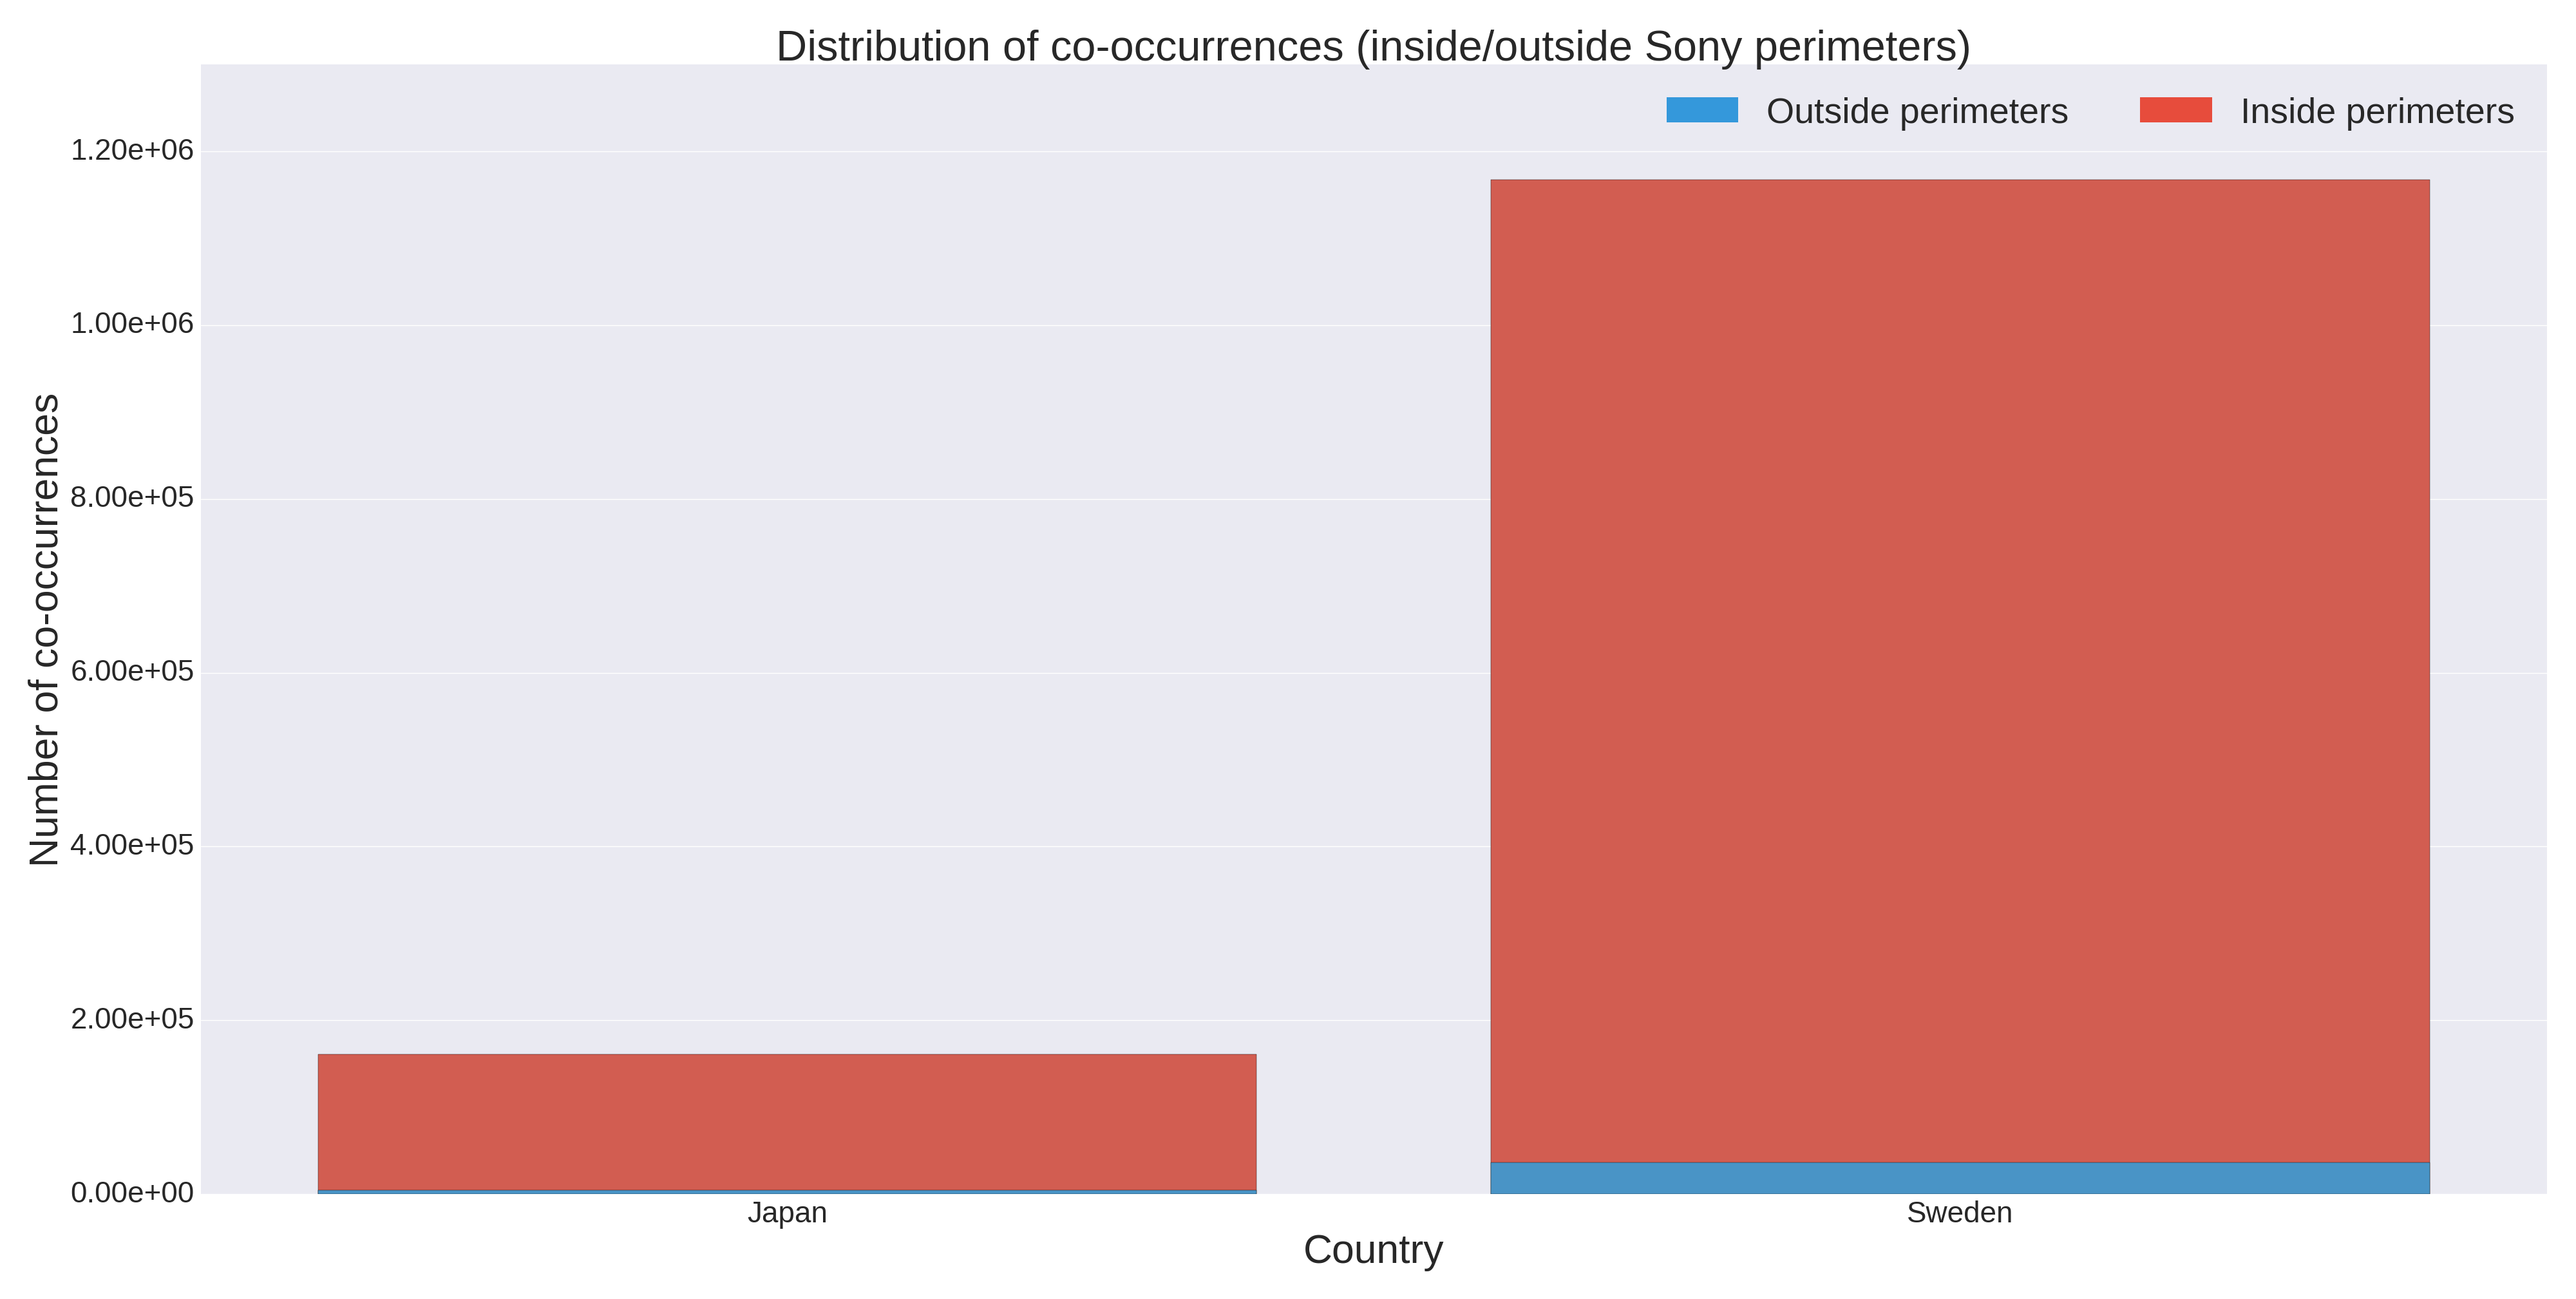
\includegraphics[scale=0.10]{stack_bar_coocs}
    \caption{Distribution of co-occurrences inside and outside Sony perimeters}
    \label{fig:dist_coocs_sony}
\end{figure}

\section{Modeling}
In this subsection we will describe the model and features used for prediction.

We will try to answer the following question: Can we predict if people meet in a period based on their spatiotemporal patterns in a previous period.
The models and algorithms we use are implemented in \textit{scikit-learn}\cite{scikit-learn} a Python module for machine learning. 

\subsection{Models}
In this thesis we will use two models, Logistic Regression and Random Forest. For each model we will first fit them on the complete period of 3 months and then the month which best met our criteria in \autoref{chap:dataset}.

\subsubsection{Logistic Regression}
The Logistic Regression model will be used as the baseline model. It will be fit on only one feature, whether or not people have had two co-occurrences in distinct spatial bins. We will compare the predictive strength of just that one feature to several different features fitted to a Random Forest model.

\subsubsection{Random Forest}
The random forest is an \textit{ensemble learning} classifier which means it fits several models to obtain better predictive performance than just a single model would achieve. In the case of the random forest it fits several decision trees. Each decision tree is fitted with a random sample with replacement of the training data, a technique called \textit{bagging}, furthermore it uses a random subset of features. The predicted class will then be the \textit{mode} of predictions of the decision trees.

In the following sections we will describe the different features which our models are fitted on.

\subsection{Spatial Features}

\subsubsection{Specificity}
The total number of co-occurrences between two users divided by the sum of the two users location updates. Feature ID: \textit{14}

\subsubsection{Number of co-occurrences}
The total number of co-occurrences between users. Feature ID: \textit{0}.

\subsubsection{Diversity of a co-occurrence}
We use the diversity measure taken from the papers of Shahabi and Pham\cite{iRWRfSD}\cite{AEBMtISSfSD}.
Diversity is a measure of how important the spatial locations of the co-occurrences between a pair of persons are, given how many times they appear.
It exists in two forms, one using Shannon entropy another using Rényi entropy, we will use Shannon. Feature ID: \textit{2}.
The Shannon entropy is defined by Equation \ref{eq:shannon_entropy}
\begin{equation}
\label{eq:shannon_entropy}
H^S_{ij}=-\sum\limits_{l}P^l_{ij} \log P^l_{ij}= -\sum\limits_{l,c_ij,l\neq 0}\frac{c_{ij,l}}{f_{ij}}\log \frac{c_{ij,l}}{f_{ij}}
\end{equation}
where $f_{ij}$, the \textit{frequency}, is the total number of co-occurrences between user $i$ and user $j$, and $c_{ij,l}$, the \textit{local frequency}, is the total number of co-occurrences between user $i$ and $j$ at location $l$.
From this the diversity is defined by taking the exponential function of the entropy defined in Equation \ref{eq:diversity}:
\begin{equation}
\label{eq:diversity}
D^s_{ij} = exp(H^S_{ij})
\end{equation}

\subsubsection{Unique co-occurrences}
The number of unique co-occurrences in terms of spatial bins between two users \textit{i} and \textit{j}. Feature ID: \textit{3}.

\subsubsection{Weighted frequency}
We use the weighted frequency measure taken from the papers of Shababi and Pham\cite{iRWRfSD}\cite{AEBMtISSfSD}.
Weighted frequency is a measure of how important the co-occurrences at non-popular places are. Feature ID: \textit{4}.
The weighed frequency is defined by Equation \ref{eq:weighted_frequency}
\begin{equation}
\label{eq:weighted_frequency}
F_{ij}=\sum\limits_{l}c_{ij,l} \times \exp(-H_l)
\end{equation}
where $H_l$ is the Location Entropy for location \textit{l} defined in Equation \ref{eq:location_entropy}
\begin{equation}
\label{eq:location_entropy}
H_l = \sum\limits_{u, P_{u,l}\neq0} P_{u,l}\log P_{u,l}
\end{equation}
where $P_{u,l}$ is the probability that a location update from location \textit{l} belongs to user \textit{u}.

\subsubsection{Co-occurrences weighted with respect to each location}
We use the weighted co-occurrences measure proposed in the master's thesis of Sapieżyński\cite{IMM2013-06556}.
The co-occurrences between users \textit{i} and \textit{j} are weighted by how many other people are present in the same spatial bin and time bin.
Feature ID: \textit{5}.

\subsubsection{Common travels}
We use the common travels measure proposed in the master's thesis of Sapieżyński\cite{IMM2013-06556}.
The number of common travels between two users. Common travels are defined when user \textit{i} and user \textit{j} co-occur in consecutive time-bins with each spatial bin being different than the previous one. Feature ID: \textit{6}.

\subsubsection{Mutual co-occurrences}
Number of mutual co-occurrences, the mutual co-occurrences for user \textit{i} and \textit{j} will be the number of users whom they share co-occurrences with. Feature ID:\textit{8}.

\subsection{Homophily Features}
Based on the work by McPherson et al.\cite{mcpherson2001birds}, we have tried to create several features based on homophily between users.

\subsubsection{Within 6 years of age}
Whether they are within 6 years of age of each other. Feature ID: \textit{9}

\subsubsection{Same gender}
Whether they are the same gender. Feature ID: \textit{10}

\subsubsection{Jaccard index similarity of used apps}
The Jaccard index is a measure used in comparing the similarity of sample sets. We extract what apps two users have used in the period and compute the similarity between them using the Jaccard index. Feature ID:\textit{13}.
The Jaccard index is defined in Equation \ref{eq:jaccard_index}
\begin{equation}
\label{eq:jaccard_index}
J(A_i,A_j) = \frac{ |A_i \cap A_j| }{ |A_i \cup A_j | }
\end{equation}
where $A_i$ is the set of apps used by user $i$ and $A_j$ is the set of apps used by user $j$. If $A_i$ and $A_j$ are empty sets we define $J(A_i, A_j) = 1$

\subsection{Temporal features}
In this section we have features related to the time of the co-occurrences.

\subsubsection{Timely arrival and leaving}
We use the timely arrival and leaving measure proposed in the master's thesis of Sapieżyński\cite{IMM2013-06556}.
Sapieżyński argued that two persons arriving or leaving a location synchronously could be more indicative of friendship than them arriving or leaving non-synchronously.
Feature ID: \textit{1}.

\subsubsection{Number of weekends}
How many co-occurrences between to users happened in the weekend, defined as either a Friday after 18:00, a Saturday or a Sunday.
Feature ID: \textit{11}.

\subsubsection{Number of evenings}
How many co-occurrences between two users happened after 18:00.
Feature ID: \textit{12}.

\section{Results}
In this section we will discuss the results of the work we have done in this thesis.

Initially we tried to infer friendship based on app usage. We did not have directed call-logs available so we could not reliably say if for example two people were calling each other. However the idea was that if we could find users with a similar timestamp and duration in an app, they could perhaps be communicating with each other either through phone calls or messaging apps. After finding user-pairs that met that criteria we try to validate them looking at their co-occurrences, were they many or few, were they off Sony properties or on, a lot of co-occurrences off sony properties could perhaps indicate a friendship. We identified the Android activity application name and package name for when a user is in a phone call called "Phone" and "package.com.android.incallui" respectively. Furthermore we identified a large number of messaging apps. We tried finding user pairs having activity in the phone app with a start time difference and end time difference of 10 seconds from each other. We looked at co-occurrences between user-pairs found this way and found that they either had a low number of co-occurrences around Sony properties or none at all.

We decided to use a meeting in a next period as a proxy for friendship.

For our training set we found 124 negative samples (did not meet) and 2331 positive samples (did meet), the high number of positive samples is due to the inclusion of location updates in the Sony properties perimeter in our training set. In our test set we found a more moderate 289 negative samples (did not meet) and 191 positive samples (did meet).
First we trained a Logistic Regression classifier which serves as our baseline classifier to compare our other model with. We trained it only with the feature num\_coocs. Next we trained a Random Forest classifier with all of our features.

Due to our imbalanced dataset, the Logistic Regression classifier we trained initially always wanted to just predict the largest prevalent class, positive, in our training dataset.

\subsection{Class Imbalance Problem}
The Class Imbalance Problem is when the total number of samples for one class greatly exceeds the number of samples for a different class. A number of techniques can be used to handle the class imbalance problem, we will use two techniques called oversampling and undersampling\cite{tan2006introduction}. In oversampling you sample the minor sample with replacement until there is an equal number of positive and negative samples. In undersampling you randomly sample from the major class N times where N is the number of minor classes.

\subsection{Performance metrics}
We utilize the precision and recall metrics for evaluating the performance of our models as well as AUC of the ROC Curve.
\subsubsection{Precision}
Precision or the positive predictive value (PPV) is a metric that measures the number of a given class that are correctly identified in proportion to the number of classes that are predicted to be that class.
\subsubsection{Recall}
Recall or the true positive rate (TPR) is a metric that measures the number of a given class that are correctly identified as that class.

In Table \ref{table:models_performance_report} we can see the performance metrics of the different classifiers for the positive (did meet) and negative class (did not meet).

\begin{table}[H]
\centering
\begin{tabular}{|c|c|c|c|c|c|c|c|c|c|c|}
\hline
\textbf{Model} & \textbf{PPV +} & \textbf{TPR +} & \textbf{PPV -} & \textbf{PPV -}   \\
\hline
Logistic Regression (num\_coocs)          & 0.86 & 0.03 & 0.00 & 0.00       \\
\hline
Random Forest (T = 10)    & 0.49 & 0.57 & 0.68 & 0.62\\
\hline
Logistic Regression (num\_coocs, balanced)          & 0.86 & 0.03 & 0.61 & 1.00      \\
\hline
Random Forest (balanced, T = 200)    & 0.44 & 0.79 & 0.71 & 0.34\\
\hline
\end{tabular}
\caption{Models performance metrics}
\label{table:models_performance_report}
\end{table}

We can further look at the number of classes correctly and incorrectly predicted using a Confusion Matrix. Figure \ref{fig:conf_matrix_log_reg} and \ref{fig:conf_matrix_random_forest} shows the confusion matrices for our two models.

\begin{figure}[H]
    \hspace*{-1.0cm}
    \centering
    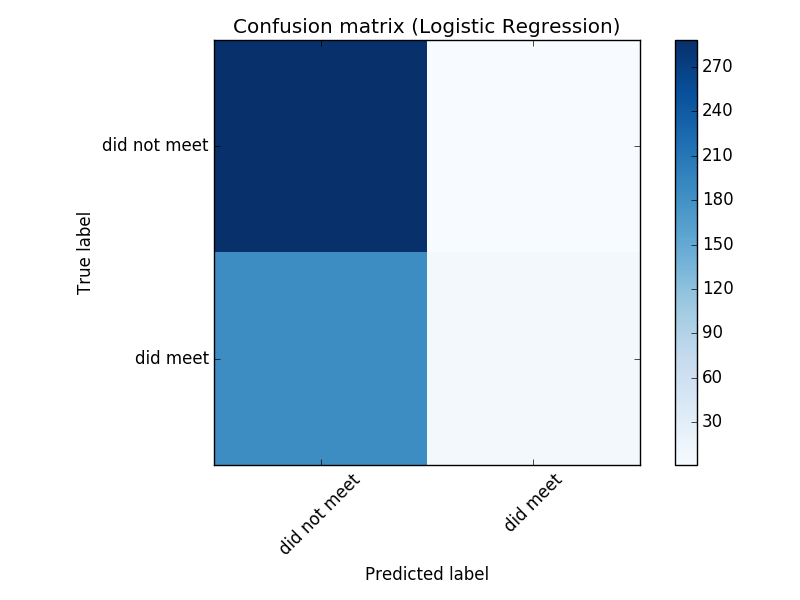
\includegraphics[scale=0.50]{confusion_matrix_log_reg}
    \caption{Confusion matrix for Logistic Regression (num\_coocs feature)}
    \label{fig:conf_matrix_log_reg}
\end{figure}
\begin{figure}[H]
    \hspace*{-1.0cm}
    \centering
    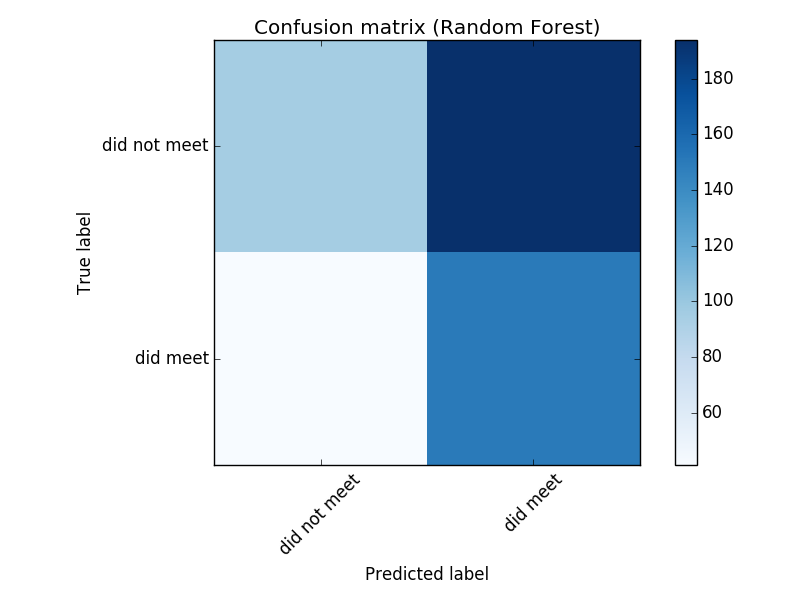
\includegraphics[scale=0.50]{confusion_matrix_random_forest}
    \caption{Confusion matrix for Random Forest (all features, 200 trees)}
    \label{fig:conf_matrix_random_forest}
\end{figure}

Looking at Figure \ref{fig:conf_matrix_log_reg} we see our baseline classifier has a very high BLABLA
We can plot the feature importances of the random forest classifier
\begin{figure}[H]
    \hspace*{-1.0cm}
    \centering
    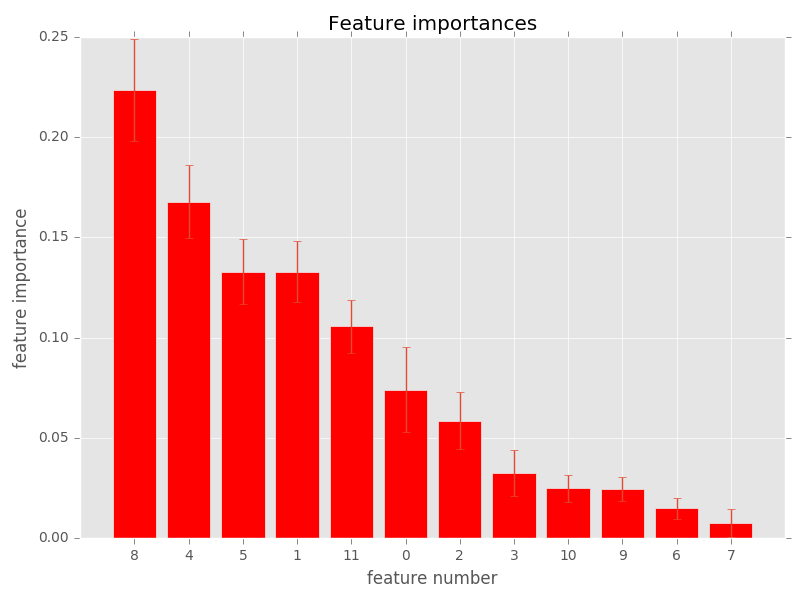
\includegraphics[scale=0.40]{feature_importances}
    \caption{Feature importances of random forest}
    \label{fig:feature_importances}
\end{figure}
\newpage
%!TEX root = main.tex
\chapter{Results}
\label{chap:results}
In this chapter we will show and discuss the results of the work we have done in this thesis.

We will start by looking at the train and test sets of the four dataset (see \autoref{tab:model_delimitation} and below) and describe what we did about class imbalance. Then we describe and interpret our results and we end the chapter with a brief summary of our findings. 

From \autoref{chap:methods} we have found the following datasets and model pairs based on the available data (see also \autoref{tab:model_overview} and \autoref{tab:model_delimitation}):
\begin{enumerate}
\item Test data
\begin{enumerate}
\item without user-filtering \\\textbf{Model pair: TP-1}
\item with user-filtering using cross-occupancy of 40\% \\\textbf{Model pair: TP-2}
\end{enumerate}
\item Production data
\begin{enumerate}
\item without user-filtering \\\textbf{Model pair: PP-1}
\item with user-filtering using cross-occupancy of 10\% \\\textbf{Model pair: PP-1}
\end{enumerate}
\end{enumerate}


For our test data without user-filtering we found a training set with 1798 negative samples (did not meet) and 9203 positive samples (did meet). In our test set we found a more moderate 5513 negative samples (did not meet) and 1674 positive samples (did meet).

Using test data with user-filtering in just September we found a training set with 118 that did not meet and 95 that did meet. The test set consisted of 151 that did not meet and 98 that did meet. 

Using production data without user-filtering we found 5585 that did not meet and 10907 that did meet for our training set, for our test set we found 9148 that did not meet and 10028 that did meet.

Using production data with user-filtering we found 403 that did not meet and 4533 that did meet for our train set and 402 that did not meet and 4630 that did meet for our test set.

The datasets composed from the test data have more negative samples than positive samples. In TP-1 the difference is more pronounced than in TP-2, except of the training set. In the production data, we have the opposite. Here we have more positive samples than negative. \\
This shows we have a class impalance problem since the dataset are imbalanced. Due to this, the Logistic Regression classifier we trained initially predicted the largest prevalent class, in our training dataset. The next section explains this problem and how we dealt with it. 


\section{Class Imbalance Problem}
\label{sec:class_imbalance_problem}
The Class Imbalance Problem is when the total number of samples for one class greatly exceeds the number of samples for a different class. A number of techniques can be used to handle the class imbalance problem, we will use two techniques called oversampling and undersampling\cite{tan2006introduction}. In oversampling you sample the minor sample with replacement until there is an equal number of positive and negative samples. In undersampling you randomly sample from the major class $N$ times where $N$ is the number of minor classes.

\section{Performance metrics}
\label{sec:performance_metrics}
We utilize the precision and recall metrics for evaluating the performance of our models as well as AUC of the ROC Curve.

\subsection{Receiver Operating Characteristic (ROC)}
The Receiver Operating Characteristic or ROC in short, illustrates the performance of a binary classifier in terms of the true positive rate (TPR, also called recall) plotted against the false positive rate (FPR) at different discrimination thresholds. As points on the ROC-curve represents different thresholds with an associated (TPR,FPR) pair it allows us to see different trade-offs between TPR and FPR. The ROC curve is useful for comparing the relative performance of different classifiers\cite{tan2006introduction} The area under the curve (AUC) represents the probability that a classifier will rank a random positive sample higher than a negative sample, assuming positive ranks higher. An AUC of 0.5 would mean the model would just randomly guess the class of each sample. We will use the ROC AUC as a metric for comparing our different models.

\subsection{Precision and Recall}
Precision or the positive predictive value (PPV) is a metric that measures the number of a given class that are correctly identified in proportion to the number of classes that are predicted to be that class.
%\subsection{Recall}
\textcolor{blue}{Recall}
Recall or the true positive rate (TPR) is a metric that measures the number of a given class that are correctly identified as that class.

In Table \ref{table:models_performance_report} we can see the performance metrics of the different classifiers for the positive (did meet) and negative class (did not meet).

\begin{table}[H]
\centering
\begin{tabular}{|c|c|c|c|c|c|c|c|c|c|c|}
\hline
\textbf{Model} & \textbf{PPV} & \textbf{TPR} & \textbf{PPV -} & \textbf{PPV -}   \\
\hline
TP-1          & 0.86 & 0.03\\
\hline
TP-2    & 0.49 & 0.57\\
\hline
PP-1          & 0.86 & 0.03\\
\hline
PP-2    & 0.44 & 0.79 &\\
\hline
\end{tabular}
\caption{Models performance metrics}
\label{table:models_performance_report}
\end{table}

We can further look at the number of classes correctly and incorrectly predicted using a Confusion Matrix. Figure \ref{fig:conf_matrix_log_reg} and \ref{fig:conf_matrix_random_forest} shows the confusion matrices for our two models.

\begin{figure}[H]
    \hspace*{-1.0cm}
    \centering
    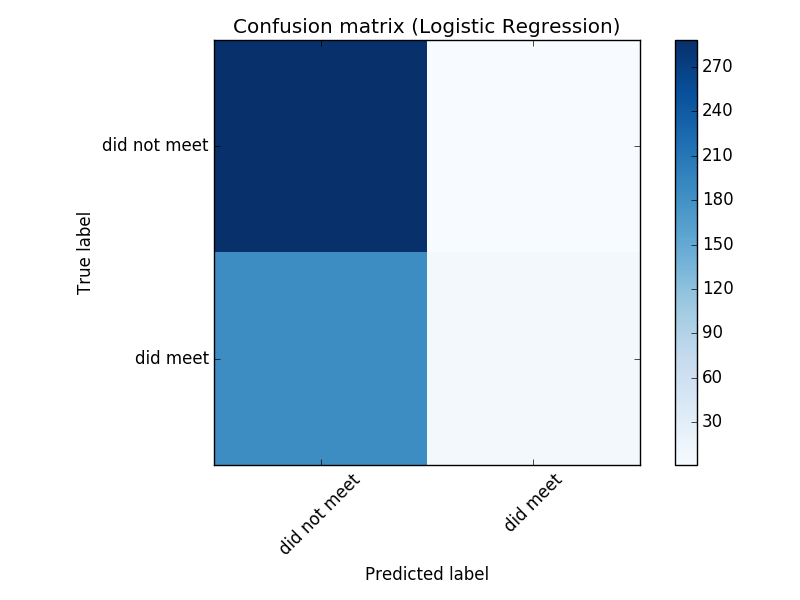
\includegraphics[scale=0.50]{confusion_matrix_log_reg}
    \caption{Confusion matrix for Logistic Regression (num\_coocs feature)}
    \label{fig:conf_matrix_log_reg}
\end{figure}
\begin{figure}[H]
    \hspace*{-1.0cm}
    \centering
    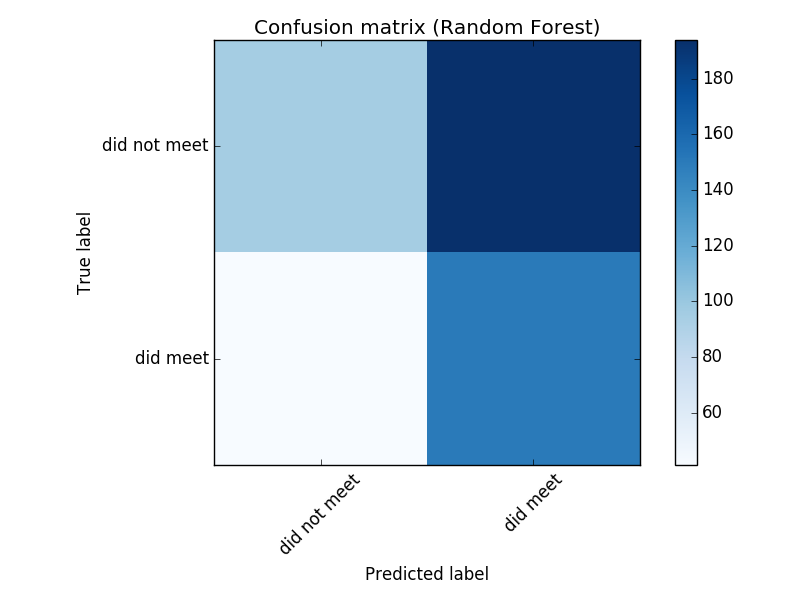
\includegraphics[scale=0.50]{confusion_matrix_random_forest}
    \caption{Confusion matrix for Random Forest (all features, 200 trees)}
    \label{fig:conf_matrix_random_forest}
\end{figure}

Looking at Figure \ref{fig:conf_matrix_log_reg} we see our baseline classifier has a very high BLABLA

\subsection{Feature importance}
We can plot the feature importances of the random forest classifier
\begin{figure}[H]
    \hspace*{-1.0cm}
    \centering
    \includegraphics[scale=0.40]{feature_importances_PP2}
    \caption{Feature importances of random forest for PP2}
    \label{fig:feature_importances}
\end{figure}

In Figure \ref{fig:rocs} we have plotted the ROC curve and ROC AUC for the different model pairs, we have also plotted the curve of a randomly guessing classifier for comparison. Figure \ref{fig:rocs_undersampling} shows the same models performance, where the datasets most prevalent class have been undersampled. We used randomized search to find the optimal hyper-parameters in the Random Forest models, choosing from \textit{gini} or\textit{entropy} and $1-9$ max features for each split. The randomized search runs for 20 iterations where each iteration performs a 3-fold cross-validation to validate the parameters of the model, we used ROC AUC as the scoring function. When the best parameters for the model are found, 2-fold cross-validation is performed to validate the model.

\begin{figure}[H]
    \hspace*{-1.0cm}
    \centering
    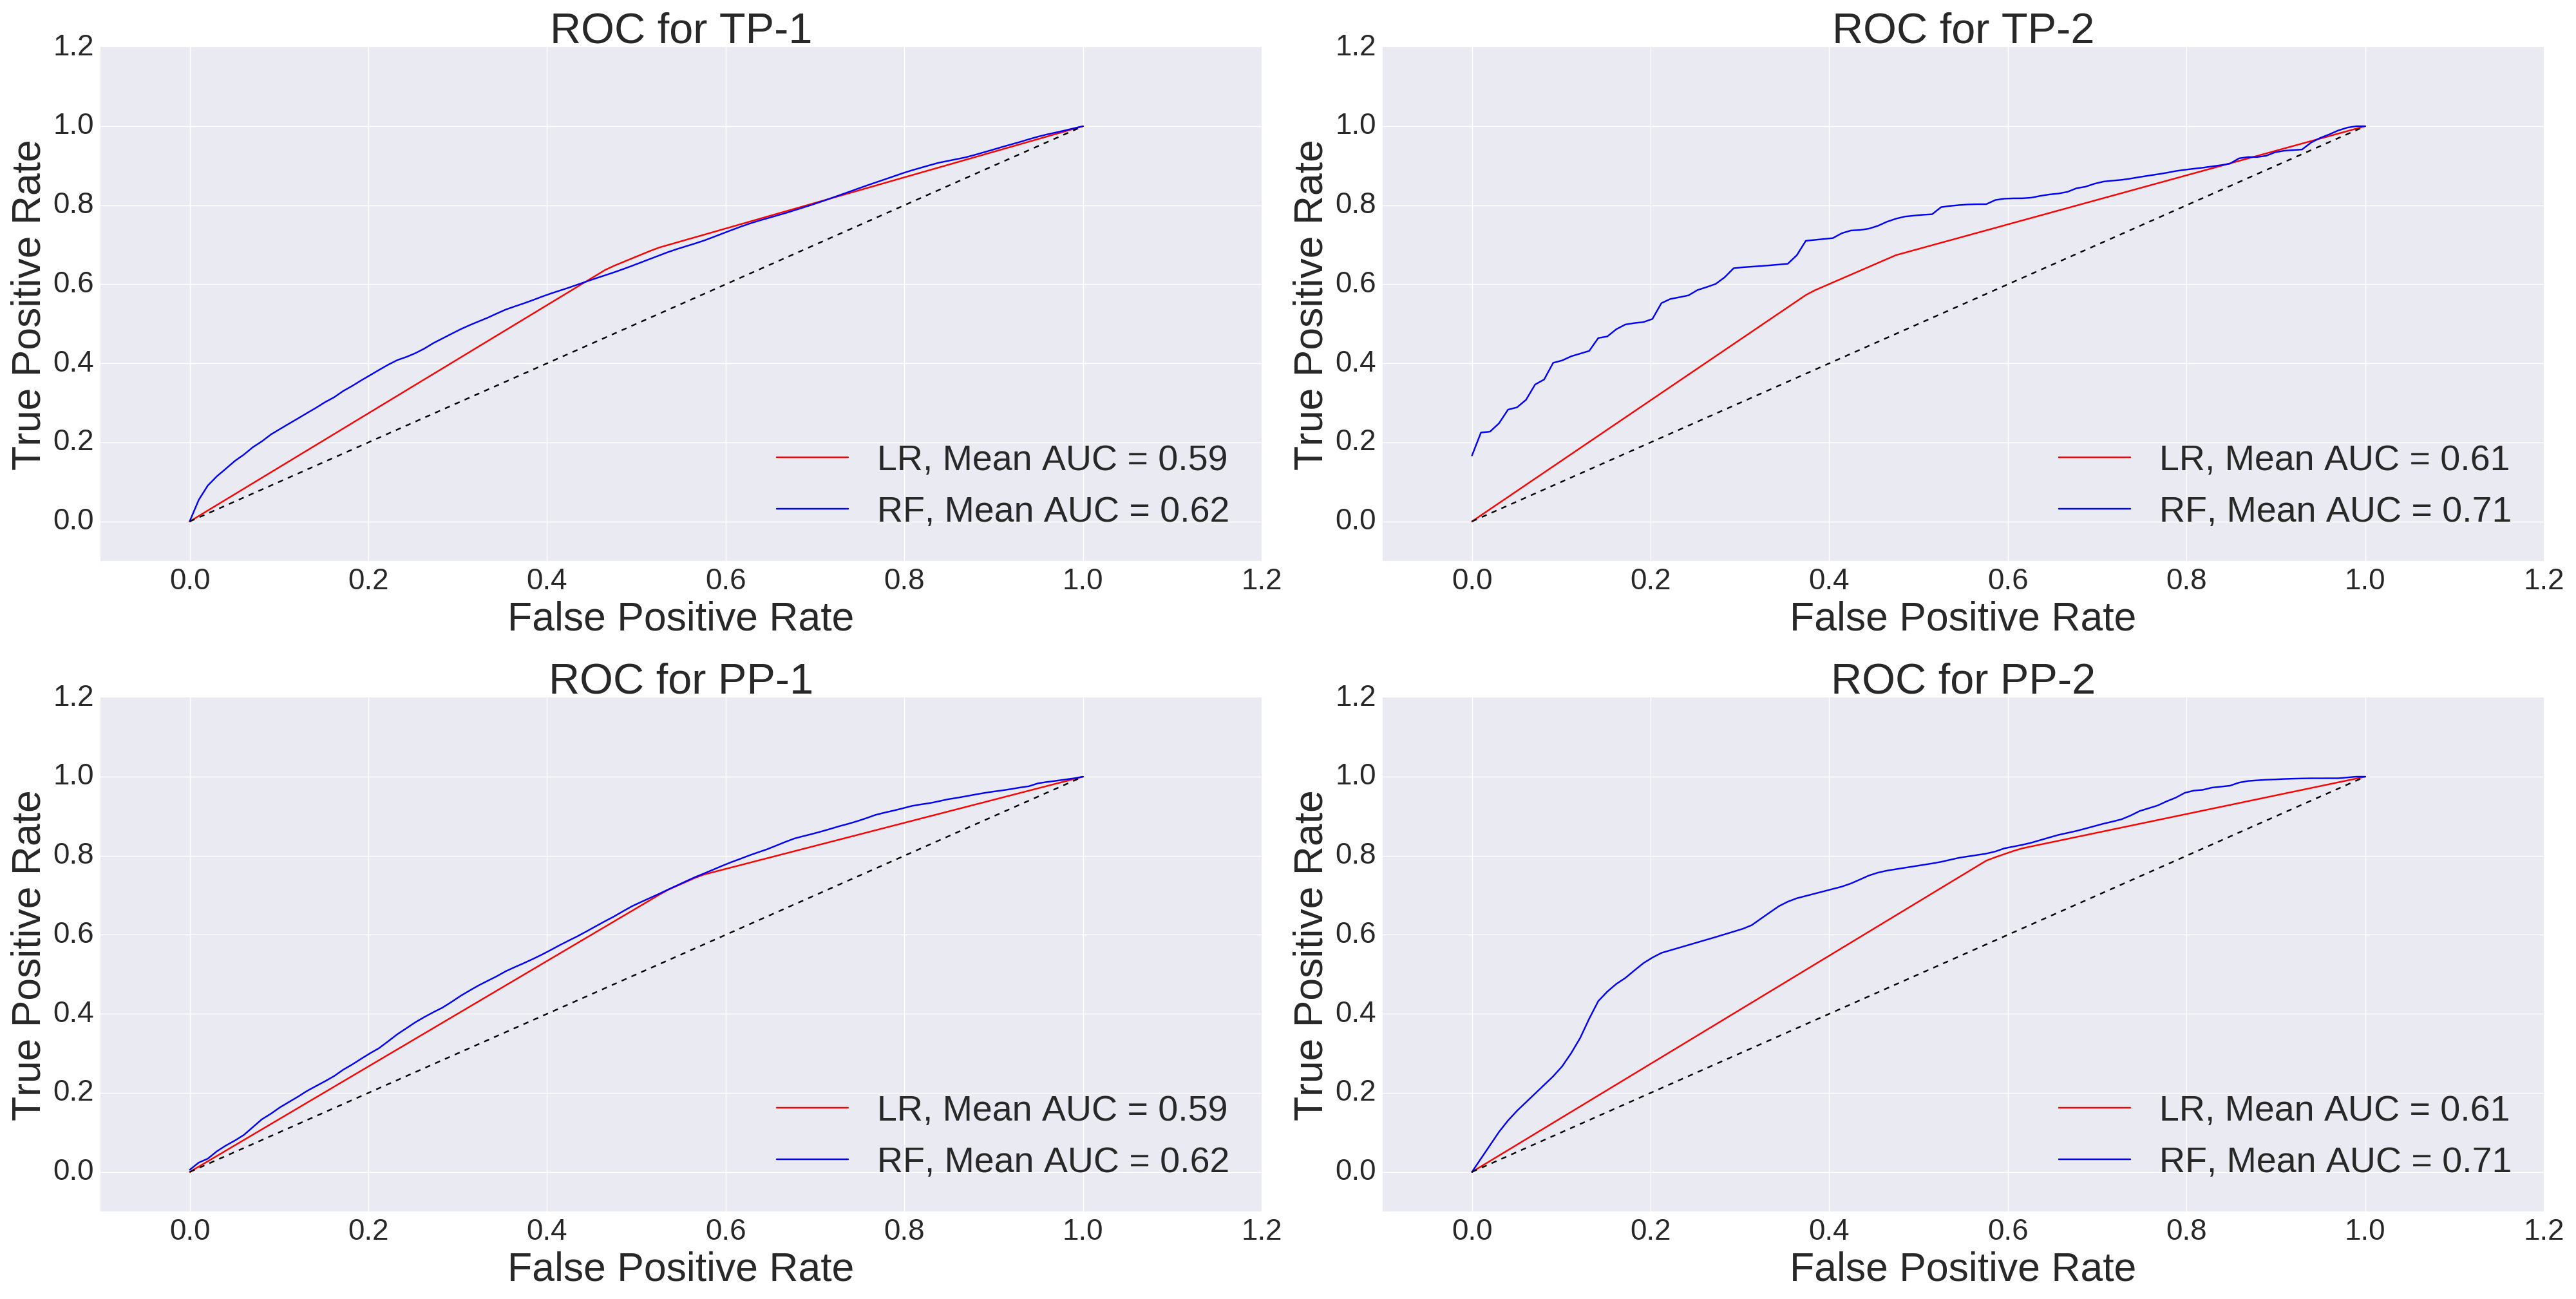
\includegraphics[scale=0.15]{ROCS}
    \caption{mean ROC AUC of Logistic Regression (LR) and Random Forest (RF) in the four model-pairs (TP-1, TP-2, PP-1, PP-2) using randomized search for hyper-parameter optimization (internal loop with 3-fold cross-validation) and 2-fold cross-validation. }
    \label{fig:rocs}
\end{figure}
\begin{figure}[H]
    \hspace*{-1.0cm}
    \centering
    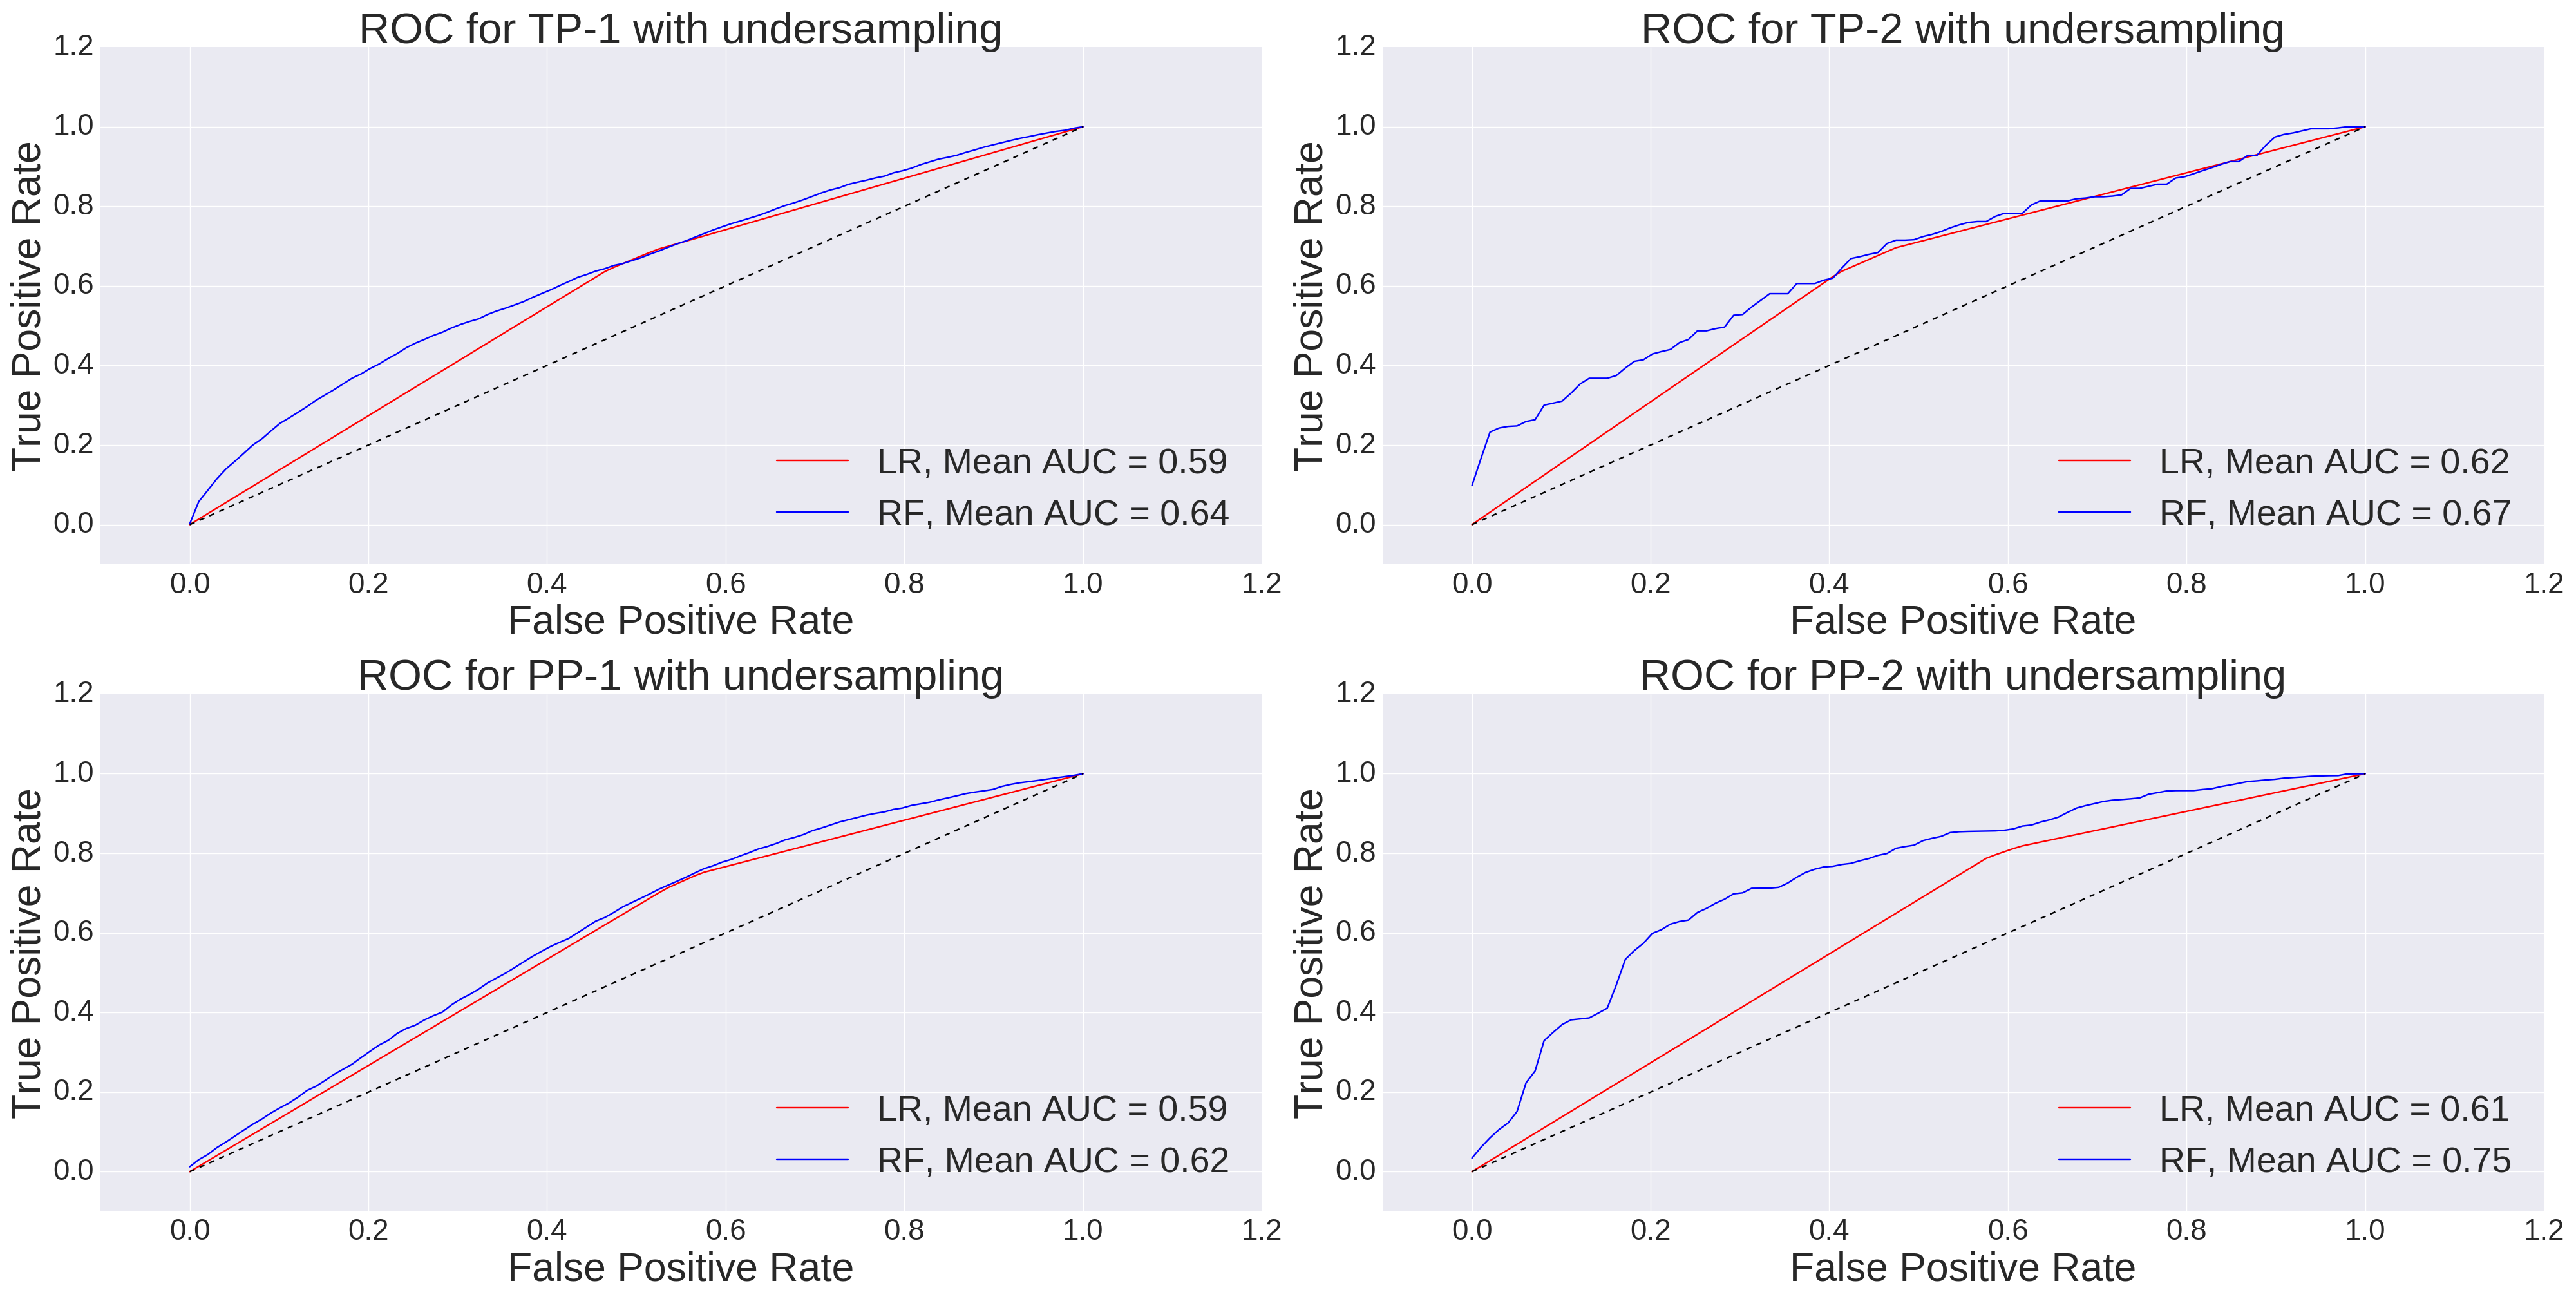
\includegraphics[scale=0.15]{ROCS_undersampling}
    \caption{mean ROC AUC of Logistic Regression (LR) and Random Forest (RF) in the four model-pairs (TP-1, TP-2, PP-1, PP-2) using randomized search for hyper-parameter optimization (internal loop with 3-fold cross-validation) and 2-fold cross-validation, and with undersampling of the most prevalent class}
    \label{fig:rocs_undersampling}
\end{figure}
\section{Summary}
\newpage
%!TEX root = main.tex
\chapter{Discussion}
In this section we will discuss the work we have done and the limitations of it.

Because of the figure of the earth being an oblate spherioid, the area of our spatial cells based on latitude and longitude degrees will vary significantly dependent on the location on the surface. The area of the cells will decrease as we traverse the globe from the equator to the poles. Equal-area partitioning like HEALPix or Quad Sphere could have been used for preserving the area measure.

The pool of users from which the data is extracted is very homogenous as it only consists of Sony employees. Future work could use a more diverse pool of users as they might exhibit different behaviours in terms of mobility and in general.

\textcolor{red}{The conclusion is that individuals who choose to reveal small amounts of public information about the times and locations of their activities may be inadvertently sending strong signals about certain of their social ties as well. [p. 5, c. 1]}
\newpage
%!TEX root = main.tex
\section{Conclusion}
                                  %Chapter 1
%\include{Chapter2}                                 %Chapter 2
\appendix
%-----------
% Backmatter
%-----------
\backmatter
\chaptermark{Bibliography}
\renewcommand{\sectionmark}[1]{\markright{#1}}
\sectionmark{Bibliography}
\addcontentsline{toc}{chapter}{Bibliography}        %Force addition of Bibliography to TOC
\bibliographystyle{alpha}                           %Use alpha codes for references
\bibliography{references}                           %Bibliography file called
%!TEX root = main.tex
\chapter{Code}
\section{main.py}
Main file for start generate datasets
\inputminted[mathescape,
               linenos,
               numbersep=5pt,
               gobble=2,
               frame=lines,
               framesep=2mm]{python}{../tools/main.py}
\section{DatabaseHelper.py}
Class for extract and insert data from/to database 
\inputminted[mathescape,
               linenos,
               numbersep=5pt,
               gobble=2,
               frame=lines,
               framesep=2mm]{python}{../tools/DatasetHelper.py}
\section{FileLoader.py}
Class for save and load the generated datasets as pickle and numpy files 
\inputminted[mathescape,
               linenos,
               numbersep=5pt,
               gobble=2,
               frame=lines,
               framesep=2mm]{python}{../tools/FileLoader.py}
\section{Predictor.py}
Class for generate datasets and make predictions
\inputminted[mathescape,
               linenos,
               numbersep=5pt,
               gobble=2,
               frame=lines,
               framesep=2mm]{python}{../tools/Predictor.py}
\section{GeoData.py}
Class for generate geo data for uset in Leaflet
\inputminted[mathescape,
               linenos,
               numbersep=5pt,
               gobble=2,
               frame=lines,
               framesep=2mm]{python}{../tools/GeoData.py}
\section{DatasetHelper.py}
Auxiliary class to generate the datasets
\inputminted[mathescape,
               linenos,
               numbersep=5pt,
               gobble=2,
               frame=lines,
               framesep=2mm]{python}{../tools/DatasetHelper.py}

\section{Appache Spark code}
Code for Apache Spark
\inputminted[mathescape,
               linenos,
               numbersep=5pt,
               gobble=2,
               frame=lines,
               framesep=2mm]{python}{../tools/template_new.py}                                 %Appendix A
\end{document}

